\documentclass[hide notes,intlimits]{beamer}

\mode<presentation>
{
  \usetheme[footline]{PISMshade}
  \setbeamercovered{transparent}
}

% load packages
\usepackage{multimedia}
\usepackage[english]{babel}
\usepackage[latin1]{inputenc}
\usepackage[T1]{fontenc}
\usepackage{lmodern}
\usepackage{pdfpages}
\usepackage[multidot]{grffile}

%\setbeameroption{show notes on second screen=right}

\usepackage{tikz}
\usetikzlibrary{shapes,arrows}
\usetikzlibrary{shadows}

\definecolor{dark red}{HTML}{E41A1C}
\definecolor{dark green}{HTML}{4DAF4A}
\definecolor{dark violet}{HTML}{984EA3}
\definecolor{dark blue}{HTML}{084594}
\definecolor{dark orange}{HTML}{FF7F00}
\definecolor{light blue}{HTML}{377EB8}
\definecolor{light red}{HTML}{FB9A99}
\definecolor{light violet}{HTML}{CAB2D6}

\setbeamercolor{boxed}{fg=black,bg=light blue!25}
\graphicspath{{figures/}}

% Define block styles
\tikzstyle{initialization} = [ellipse, draw, 
    text badly centered, draw=dark violet,
        % The filling: 
        top color=white, 
        bottom color=dark violet]
\tikzstyle{initialization faded} = [ellipse, draw, 
    text badly centered, draw=dark violet!50,
        % The filling: 
        top color=white, 
        bottom color=dark violet!25]
\tikzstyle{hindcast} = [ellipse, draw,
    text badly centered, rounded corners,draw=dark orange,
        % The filling: 
        top color=white, 
        bottom color=dark orange]
\tikzstyle{hindcast faded} = [ellipse, draw,
    text badly centered, rounded corners,draw=dark orange!50,
        % The filling: 
        top color=white, 
        bottom color=dark orange!25]
\tikzstyle{forecast} = [ellipse, draw,
    text badly centered, rounded corners,draw=dark blue,
        % The filling: 
        top color=white, 
        bottom color=dark blue]
\tikzstyle{forecast faded} = [ellipse, draw,
    text badly centered, rounded corners,draw=dark blue!50,
        % The filling: 
        top color=white, 
        bottom color=dark blue!50]
\tikzstyle{arrow line} = [draw, -latex']
\tikzstyle{line} = [draw]

\newenvironment{transbox}[1][]{%
\begin{tikzpicture}
\node[drop shadow,rounded corners,text width=.9\textwidth,fill=white, fill opacity=#1,text opacity=1] \bgroup
}{
\egroup;\end{tikzpicture}} 

\newenvironment{transbox-tight}{%
\begin{tikzpicture}
\node[drop shadow,rounded corners,fill=uaf yellow, fill opacity=0.75,text opacity=1] \bgroup
}{
\egroup;\end{tikzpicture}} 

\newcommand{\jl}{[\![}
\newcommand{\jr}{]\!\hskip 0.003cm ]}
\newcommand{\bpsi}{\boldsymbol{\psi}}
\newcommand{\bPsi}{\boldsymbol{\Psi}}
\newcommand{\bphi}{\boldsymbol{\phi}}
\newcommand{\bPhi}{\boldsymbol{\Phi}}
\newcommand{\bn}{\mathbf{n}}
\newcommand{\bq}{\mathbf{q}}
\newcommand{\bv}{\mathbf{v}}
\newcommand{\D}{\,\mathrm{d}}
\newcommand{\Tsnow}{T_{\text{snow}}}
\newcommand{\Hatm}{H_{\text l}^{\text{atm}}}

\newcommand{\mathtext}[1]{\mathsf{#1}}

% title page
\title[Ice sheet modeling] % (optional, use only with long paper titles)
{Understanding the Greenland ice sheet\\through observations and models}
%\subtitle{Understanding ice sheet response to climate change through observations and models}

\author[Aschwanden] % (optional, use only with lots of authors)
{Andy Aschwanden}
% - Give the names in the same order as the appear in the paper.
% - Use the \inst{?} command only if the authors have different
%   affiliation.

% - Use the \inst command only if there are several affiliations.
% - Keep it simple, no one is interested in your street address.

\titlegraphic{\vskip-1.cm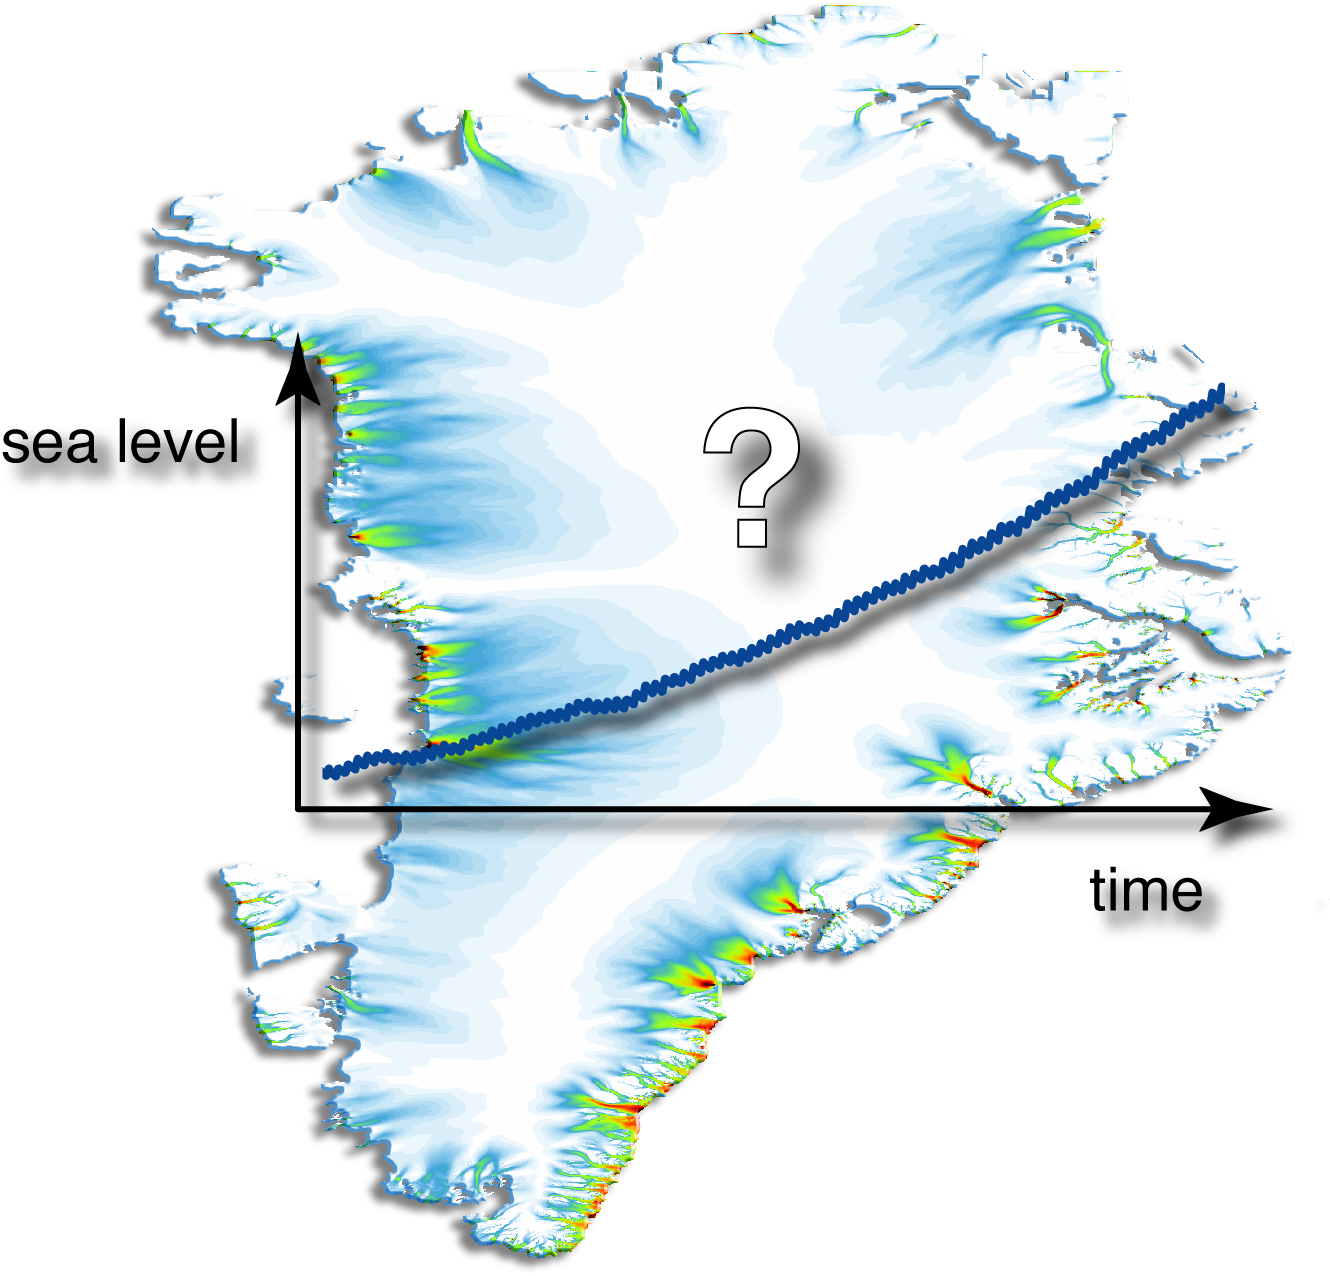
\includegraphics[height=3cm]{grn1km_speed_slr}}

\date{}


\subject{Ice sheet modeling}

\begin{document}


\setbeamertemplate{background canvas}
  {
     \tikz{\node[inner sep=0pt,opacity=1.0] {\includegraphics[width=\paperwidth]{uaf_beamer_shade_bg}};}
} 

% insert titlepage
\begin{frame}
  \titlepage
\end{frame}

\setbeamertemplate{background canvas}
  {
} 

\setbeamertemplate{background canvas}
  {
     \tikz{\node[inner sep=0pt,opacity=1.] {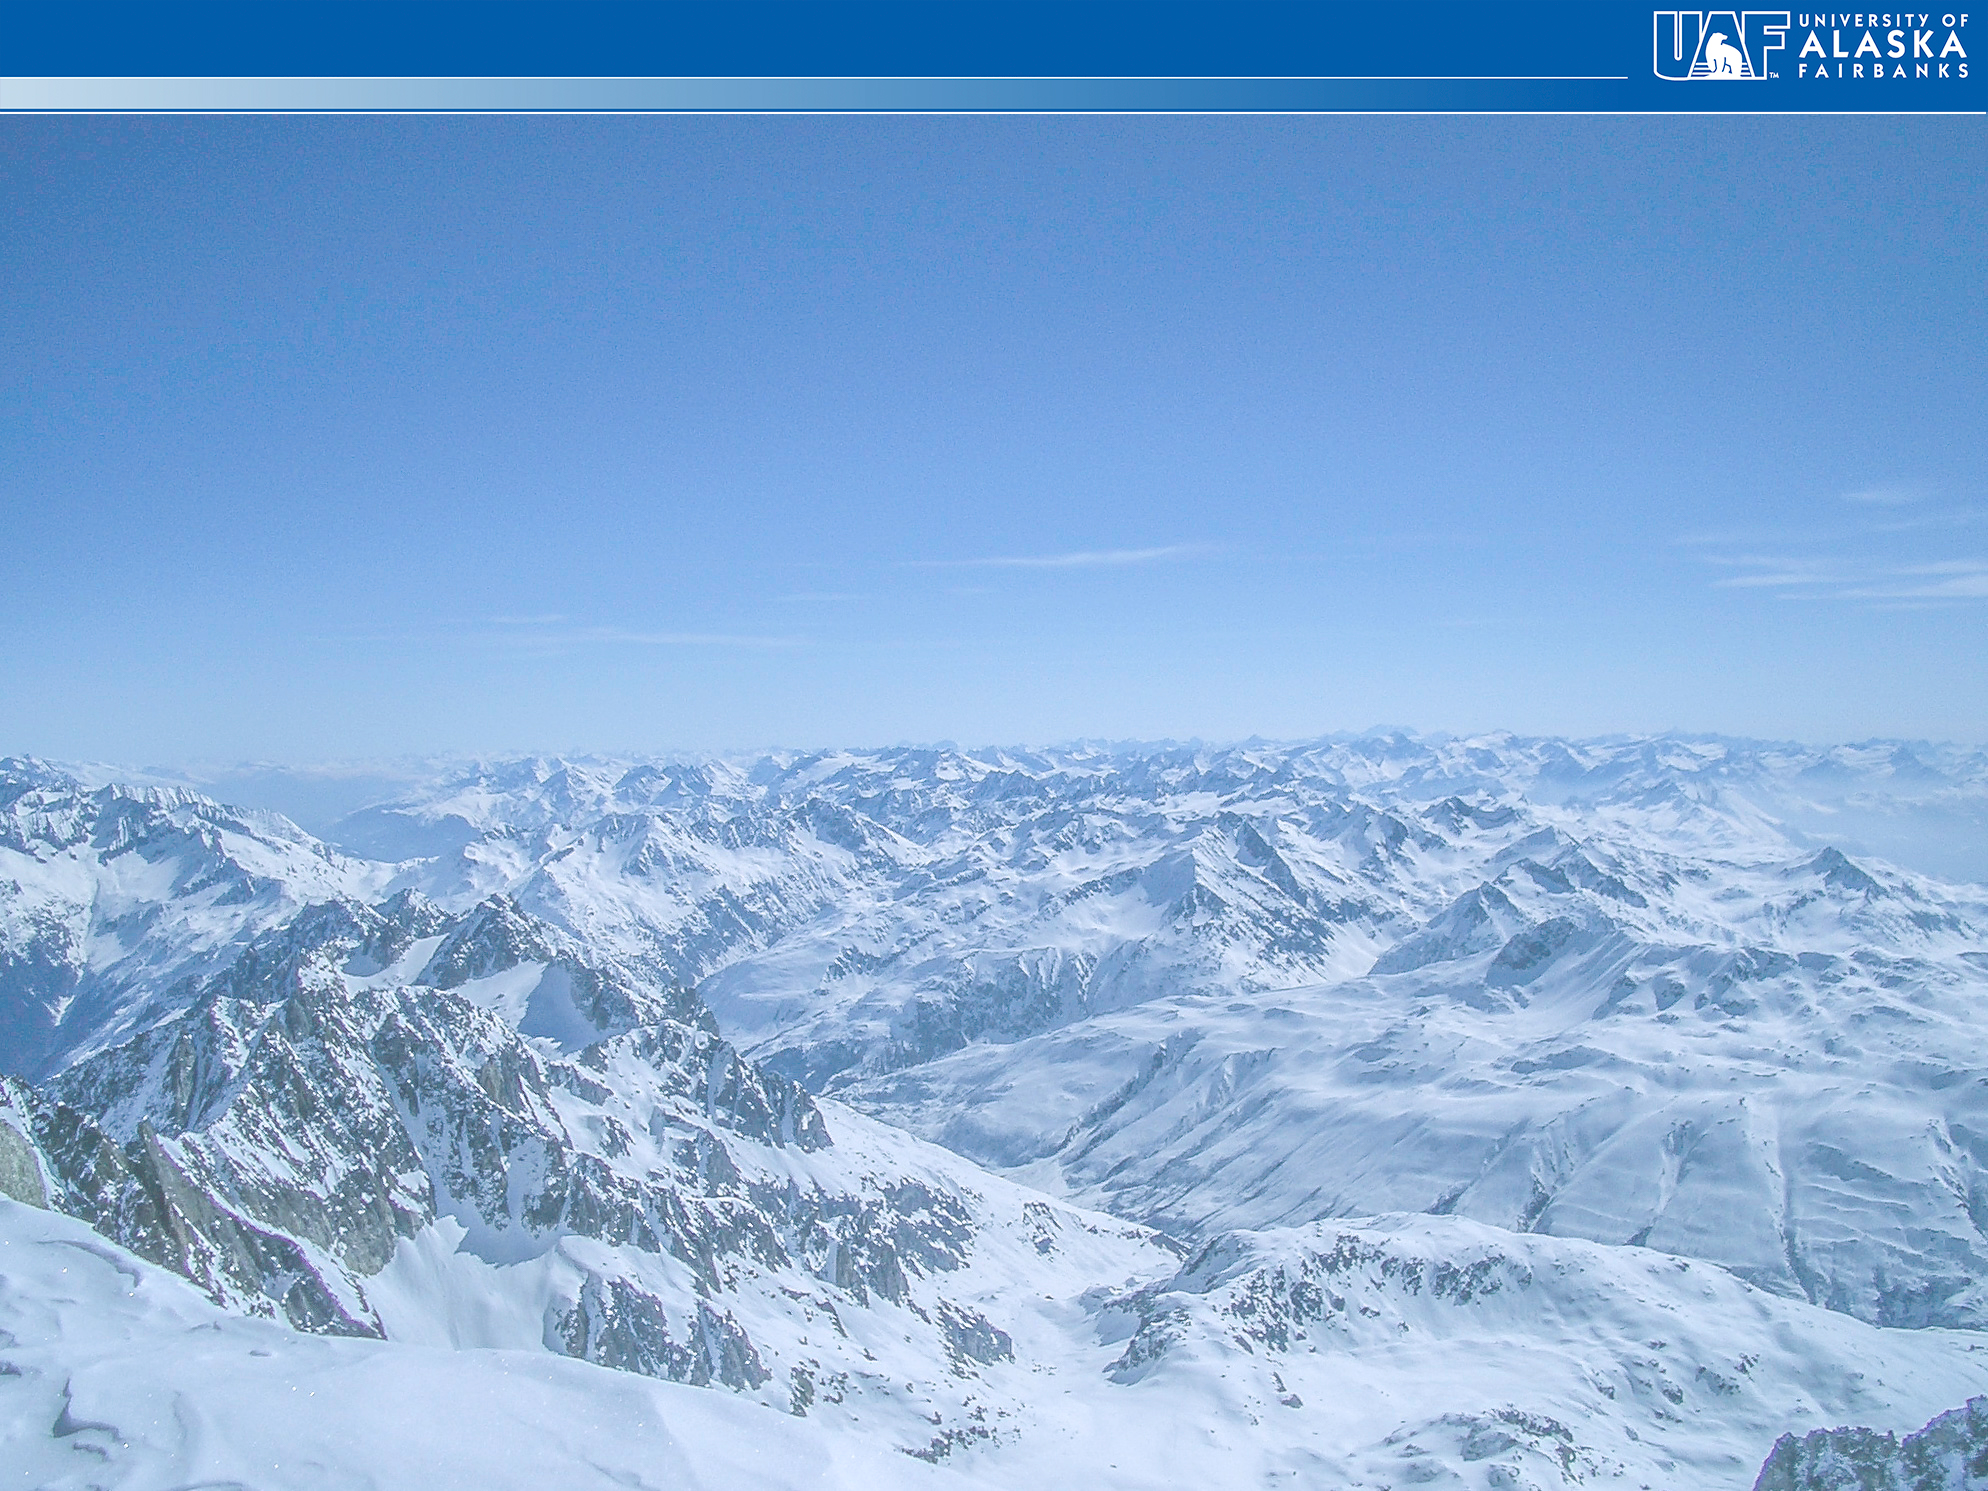
\includegraphics[width=\paperwidth]{galenstock_bg}};}
}

\begin{frame}[plain]
  \note[item]{Who has ever seen a glacier?}
  \note[item]{Who has ever set foot on a glacier?}
  \note[item]{The picture here shows the view from on of my favorite places near}
  \note[item]{where I grew up}
\end{frame}

\setbeamertemplate{background canvas}
  {
} 


\setbeamertemplate{background canvas}
  {
     \tikz{\node[inner sep=0pt,opacity=1.] {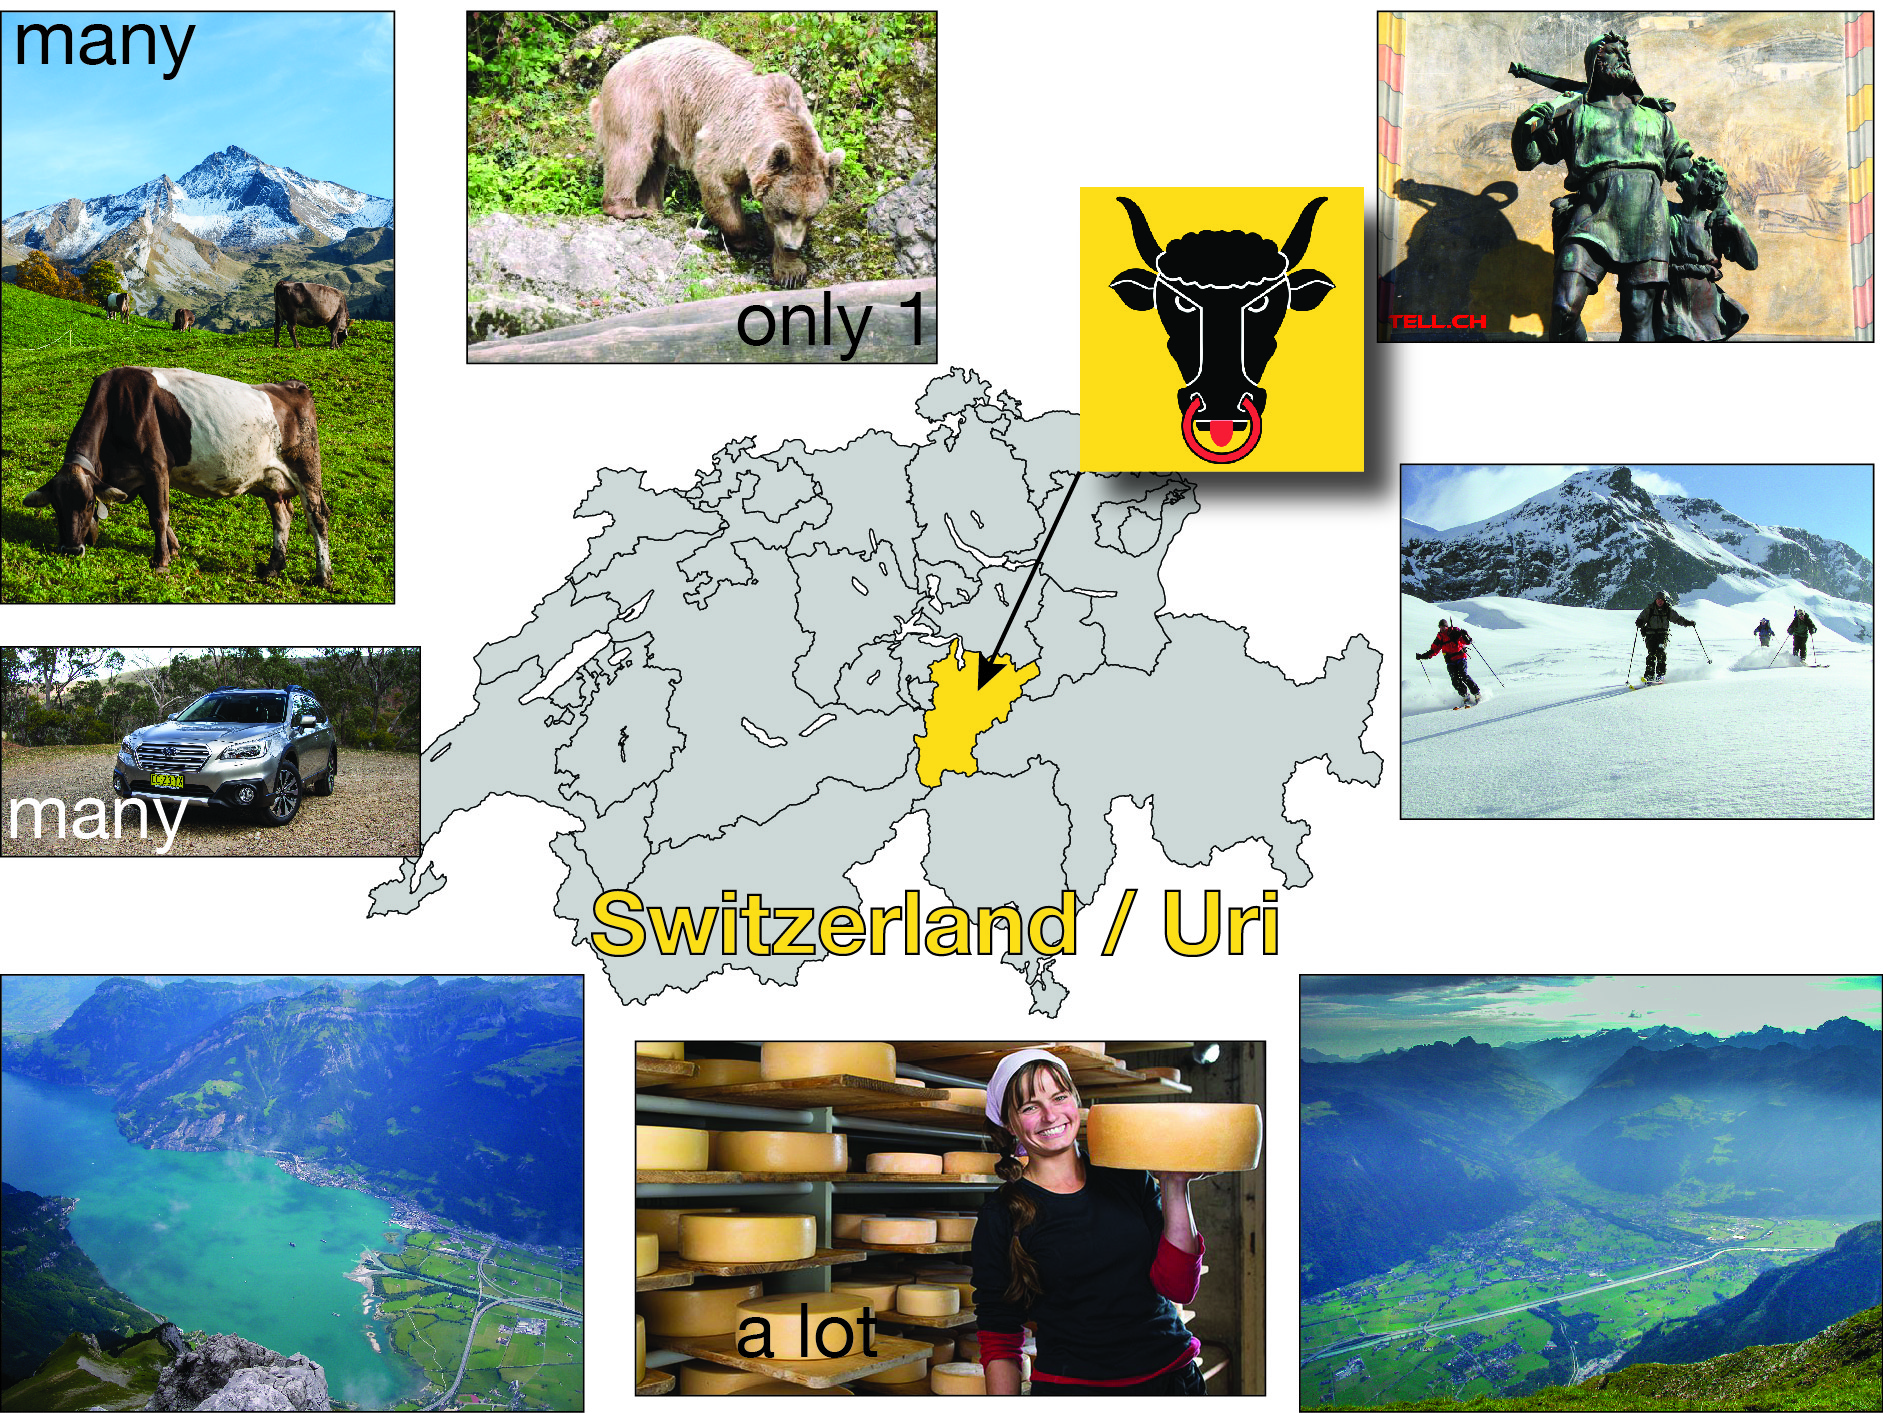
\includegraphics[width=\paperwidth]{uri-collage}};}
}

\begin{frame}[plain]
  \note[item]{I've been living in Alaska for the past nine years.}
  \note[item]{I grew up in the heart of Switzerland, in the Kanton Uri---a Kanton is the equivalent to a State}
  \note[item]{Like Alaska, we have many Subarus}
  \note[item]{True to the stereotype, we have many cows in Uri and produce a lot of good cheese}
  \note[item]{Last year we had on bear roaming through Uri, which gave it some Alaska-feel}
  \note[item]{The last bear was shot in Uri in 1820 and you can still see the claws mounted to a house}
  \note[item]{According to legend, William Tell was born in Uri, who freed us from the Austrian oppression in 1291}
  \note[item]{But first and foremost have a lot of mountains to climb and to ski}
\end{frame}

\setbeamertemplate{background canvas}
{
  \tikz{\node[inner sep=0pt,opacity=1.] {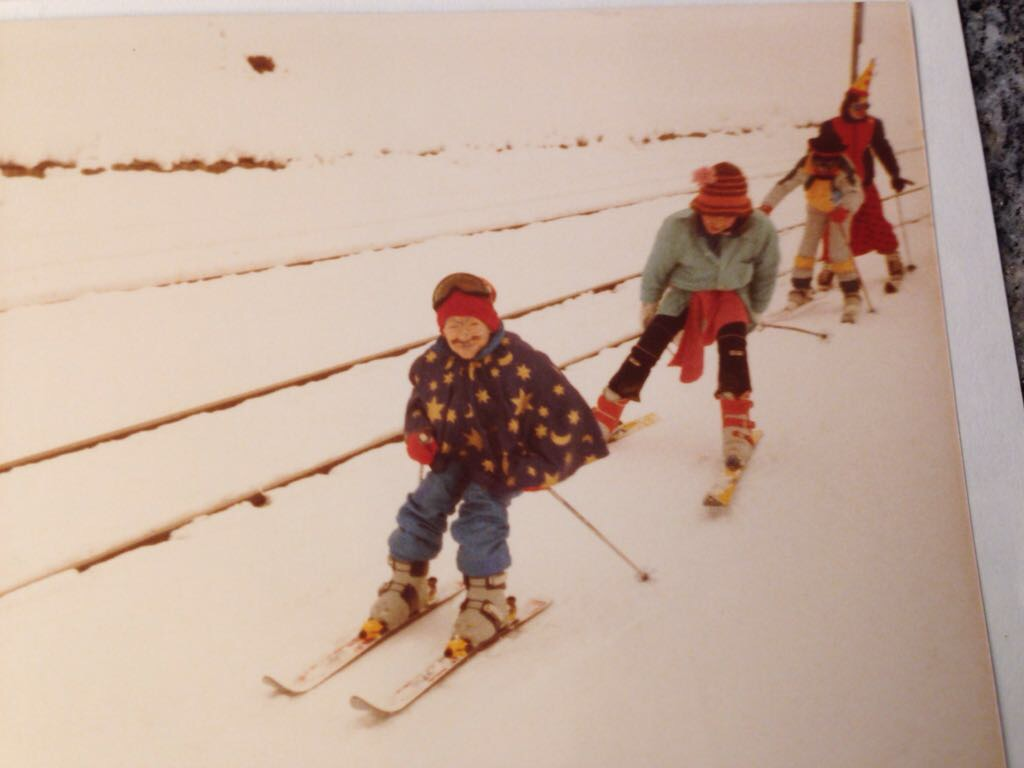
\includegraphics[width=\paperwidth]{andy-ski}};}
}

\begin{frame}[plain]
  \note[item]{So no surprise}
  \note[item]{I grew up on skis, I learned to downhill ski right after learning to walk}
  \note[item]{In Switzerland ``skiing'' always means downhill skiing, unlike in Alaska where skiing usually means XC skiing}
\end{frame}



\setbeamertemplate{background canvas}
{
  \tikz{\node[inner sep=0pt,opacity=1.] {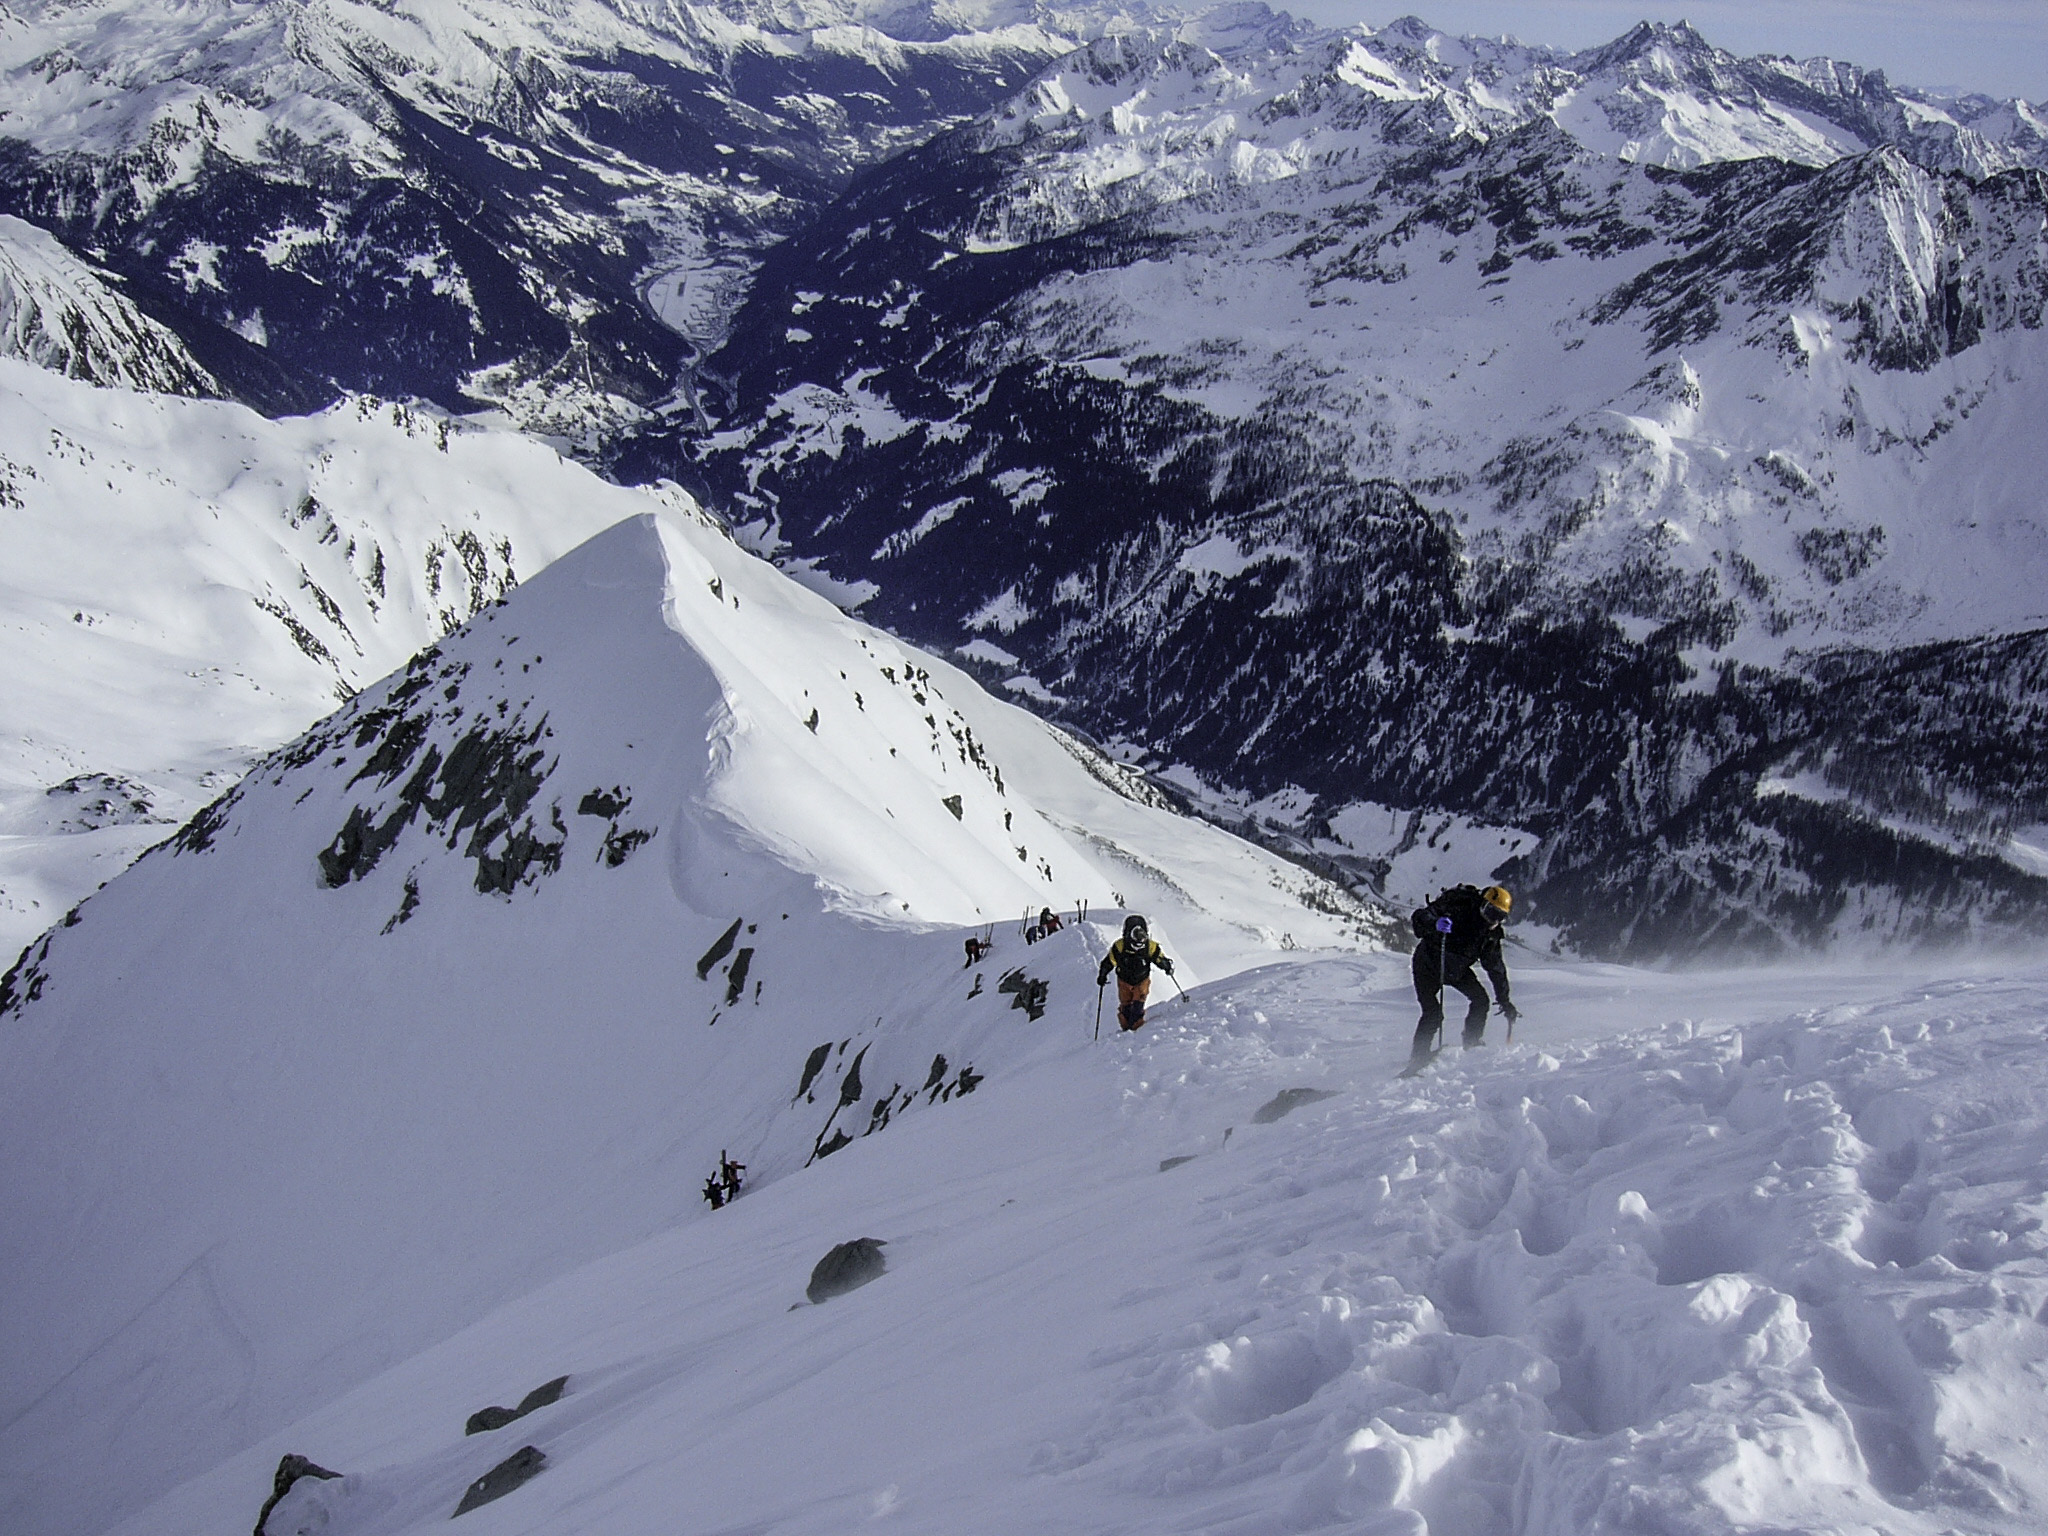
\includegraphics[width=\paperwidth]{ski-climb}};}
}

\begin{frame}[plain]
  \note[item]{When I was a bit older, I became tired of waiting for the next gondola}
  \note[item]{so started with ski mountaineering}
  \note[item]{and while spending my weekends in the mountains,}
  \note[item]{I started to notice change}
\end{frame}

\setbeamertemplate{background canvas}
{
  \tikz{\node[inner sep=0pt,opacity=1.] {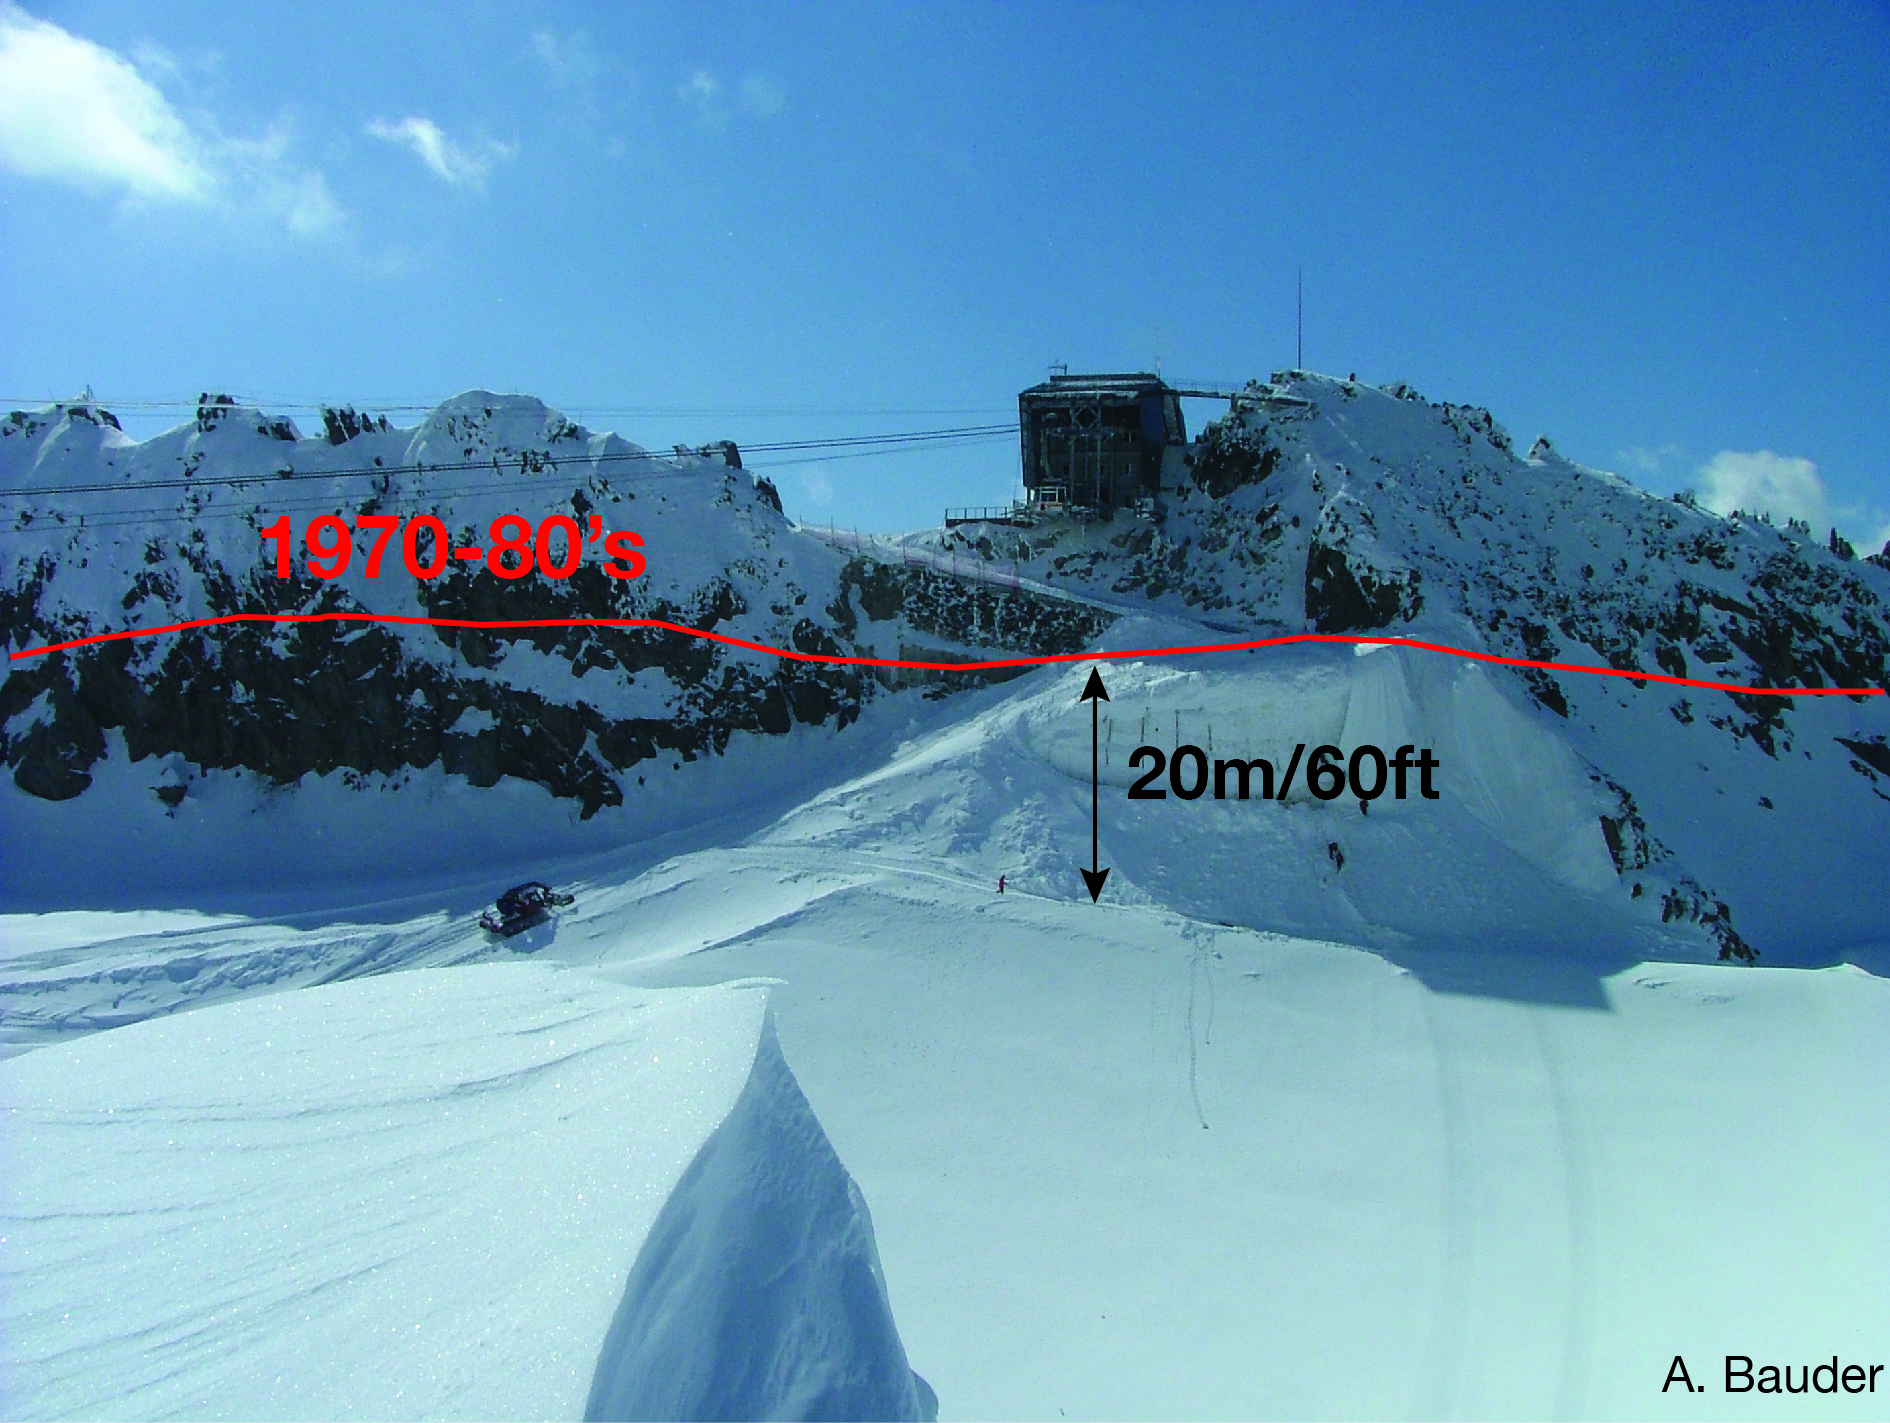
\includegraphics[width=\paperwidth]{gurschen-bauder}};}
}


\begin{frame}[plain]
  \note[item]{For example, when I was little we got out of the gondola}
  \note[item]{and we started to ski right on the glacier}
  \note[item]{However, in the past 2 or 3 decades, the glacier thinned by 20\,m or more}
  \note[item]{To get skiers on the glacier, they have to build a ramp out of snow every year}
  \note[item]{This is quite labor intensive and requires a lot of gas}
  \note[item]{Now, every spring ski patrol covers the ramp with a white tarp to preserve as much as possible}
  \note[item]{for the next winter}
  \note[item]{I asked myself: Are glaciers melting only where I grew up or is there more to it?}
  \note[item]{Is this happens somewhere else?}
  \note[item]{so, to answer this, I decided to study glaciers and climate}
  \note[item]{but also it sounded like fun to study something that I can ski on\ldots}
  \note[item]{So during the rest of talk, I would like focus on glacier change in Greenland}
  \note[item]{which is currently my main research focus}
\end{frame}
  

\setbeamertemplate{background canvas}
{
} 


\setbeamertemplate{background canvas}
  {
     \tikz{\node[inner sep=0pt,opacity=.75] {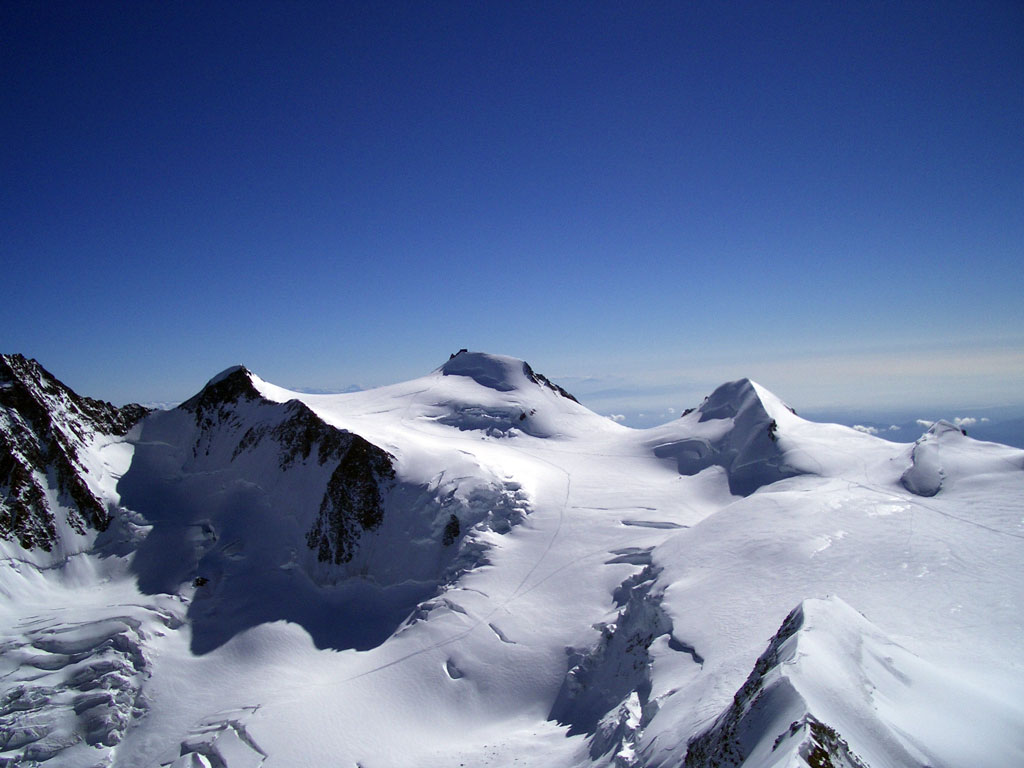
\includegraphics[height=
\paperheight,width=\paperwidth]{colle}};}
} 

\begin{frame}[plain]
  \begin{transbox}[0.5]
    \begin{block}{What is an ice sheet?}
      \begin{itemize}[<+- | alert@+>] % some control parameters
      \item Artists, Tourists: beautiful landscape
      \item Geographers: element of landscape
      \item Geologists: soft rock, sediment
      \item Hydrologists: water reservoir
      \item Climatologists: subsystem of climate system, climate archive
      \item Physicists: thermomechanical non-Newtonian fluid
      \item Mathematicians: free boundary problem in fluid dynamics
      \item Electrical engineers: one sided accessible dielectric
      \item Glaciologists: part of the cryosphere
      \end{itemize} 
    \end{block}
  \end{transbox}
  \note[item]{Well, before we start talking about ice sheets, we need to ask the question: ``What is an ice sheet''?}
  \note[item]{Depending on who you ask, you may get quite different answers.}
\end{frame}

\setbeamertemplate{background canvas}
{
%
} 



\setbeamertemplate{background canvas}
  {
     \tikz{\node[inner sep=0pt,opacity=1] {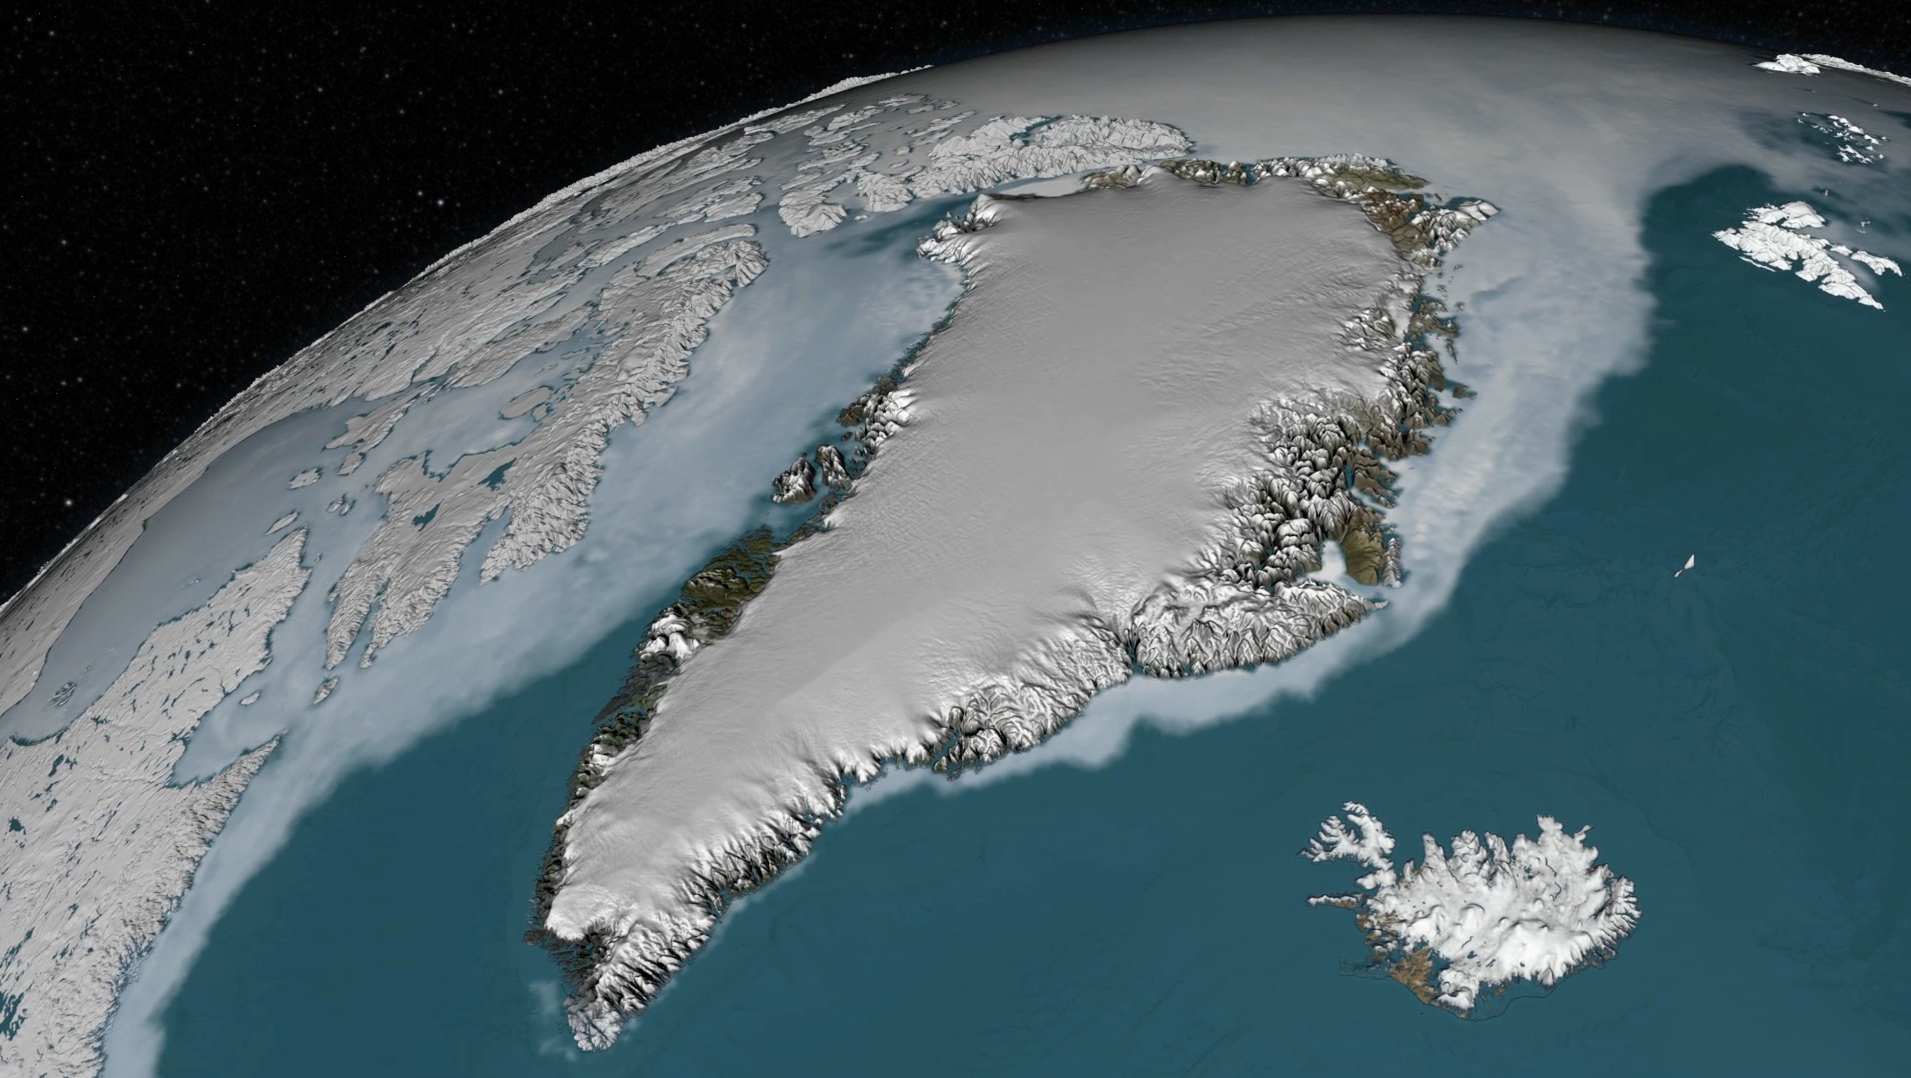
\includegraphics[height=\paperheight,width=\paperwidth]{nasa-mapping-greenland-ice-sheet}};}
} 

\begin{frame}[plain]
\end{frame}

\setbeamertemplate{background canvas}
  {
     \tikz{\node[inner sep=0pt,opacity=.5] {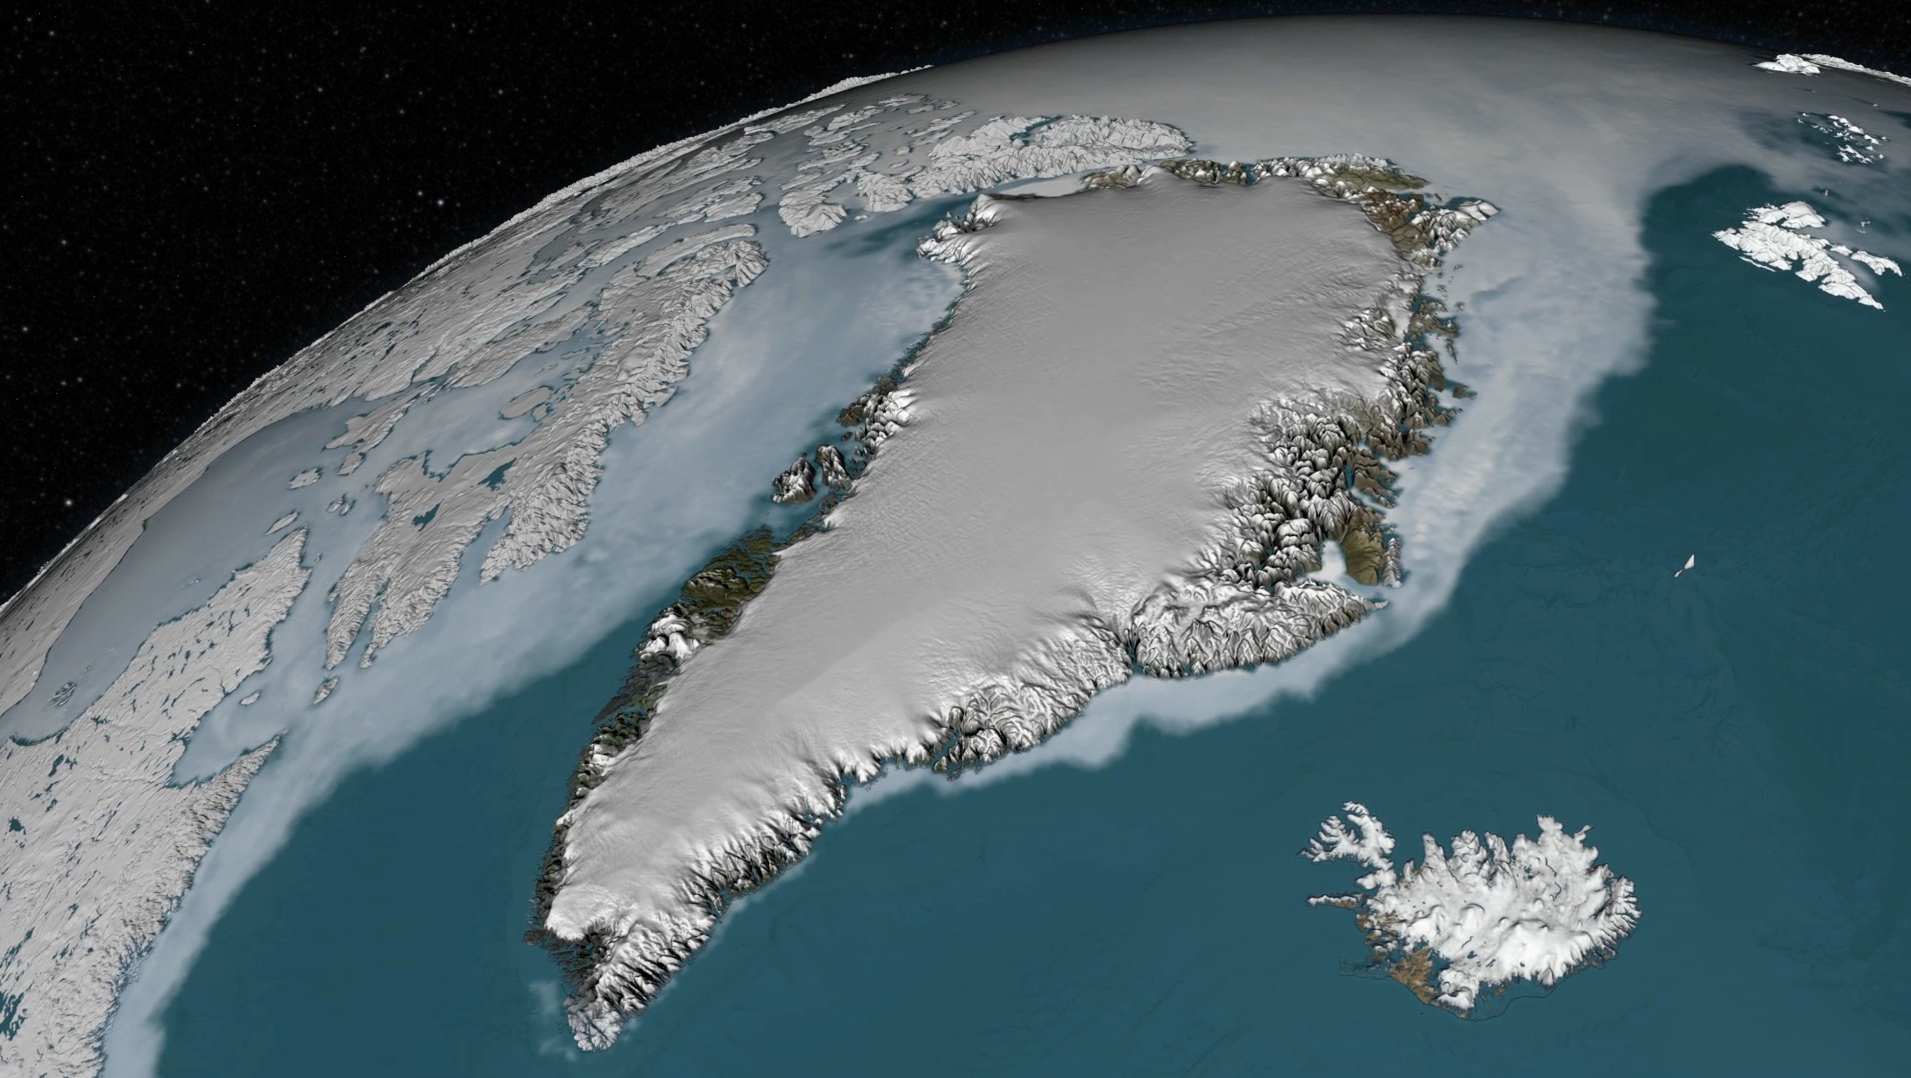
\includegraphics[height=\paperheight,width=\paperwidth]{nasa-mapping-greenland-ice-sheet}};}
} 

\begin{frame}[plain]
    \begin{itemize}
    \item extent of $1200\,\text{km}\,\times 2400\,\text{km}$ \dots it's a ``dwarf continent''
    \item total area: 2.1 million km$^2$
    \item ice covered area:  1.7 million km$^2$
    \item \alert{for comparison: that's 17$\times$ the area of South Korea}
    \item has ice equivalent of 7.2 m of sea-level rise
    \item over past 2 decades: losing mass at an accelerating rate
    \end{itemize}
    \note[item]{Explain why Greenland is of interest}
\end{frame}


\setbeamertemplate{background canvas}
{
%
} 

\begin{frame}[plain]
    \begin{figure}
      \movie[showcontrols=true,loop,width=12cm]{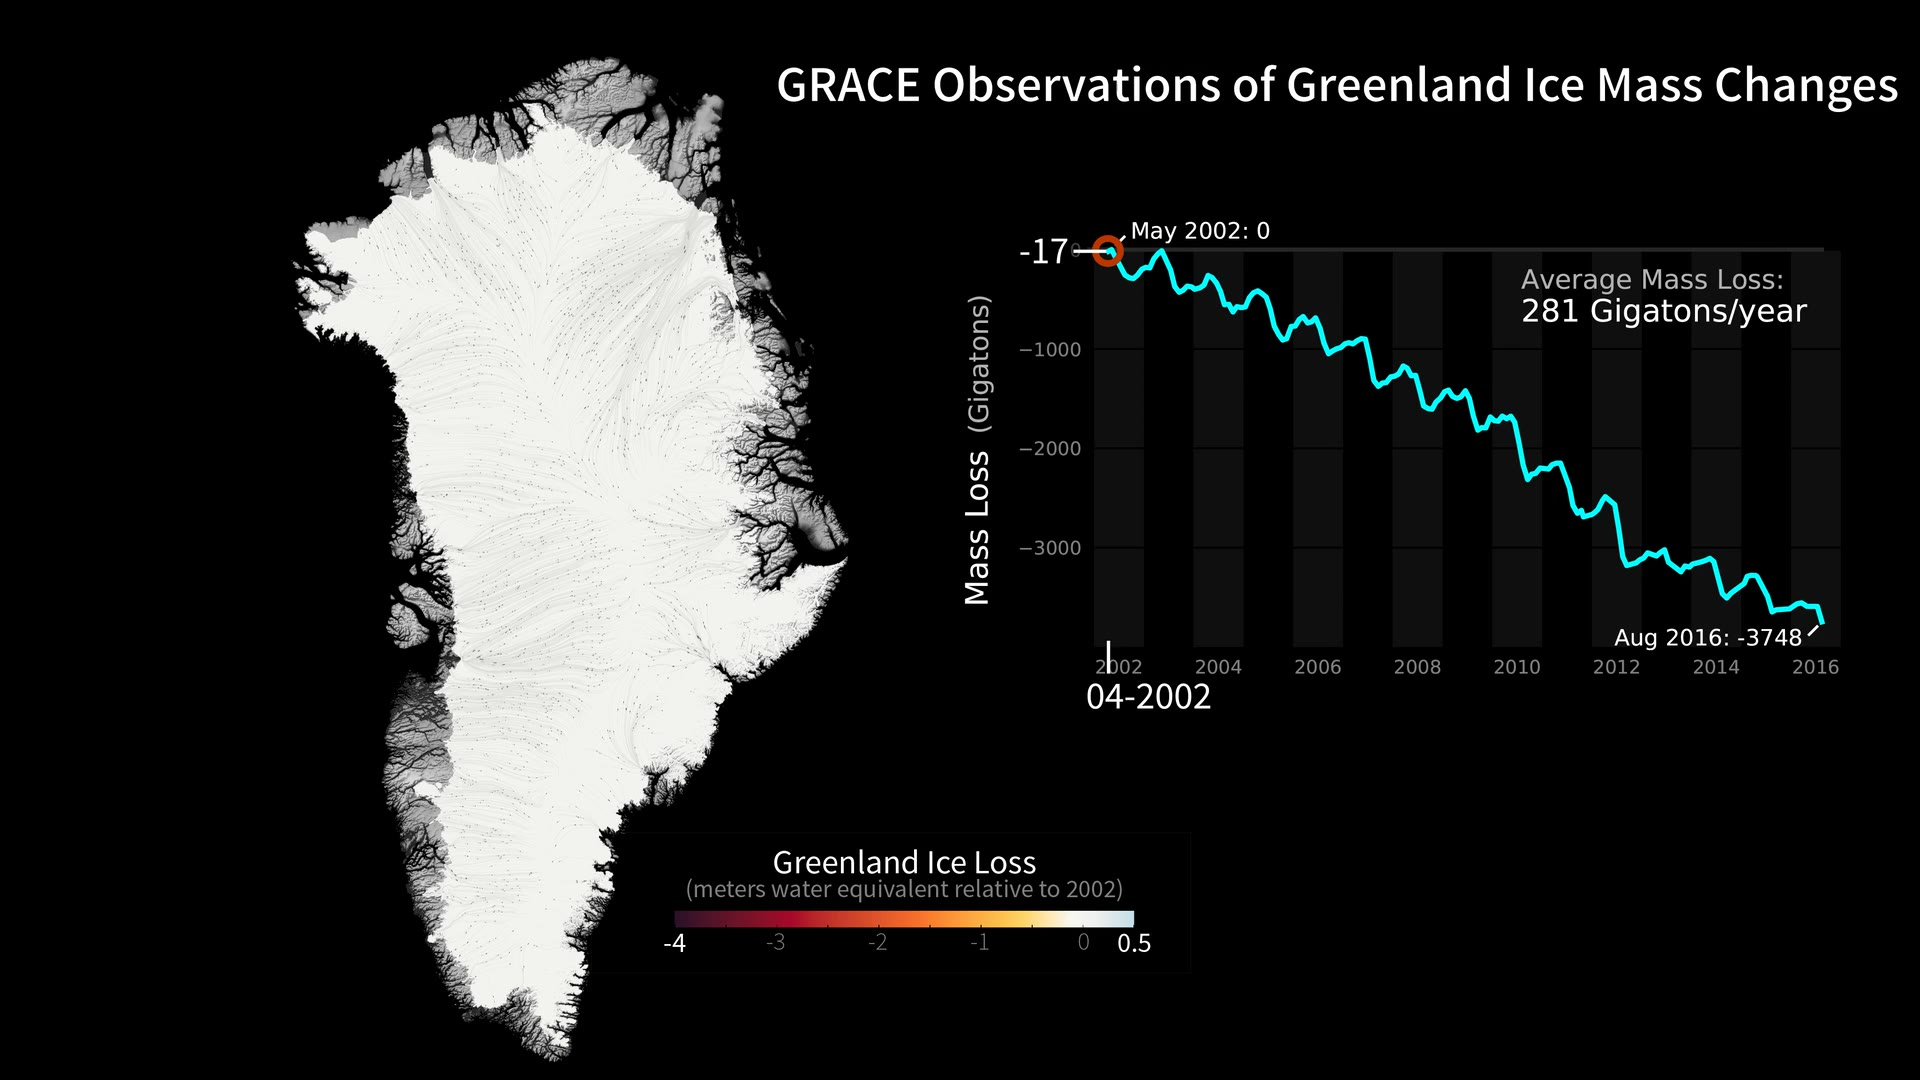
\includegraphics[width=12cm]{../movies/68_grace_greenland_1080p}}{../movies/68_grace_greenland_1080p.mov}
  \end{figure}
  \begin{itemize}
  \item<2> 280\,Gt is about half of Lake Eerie or a 3\,m high layer of water covering South Korea
  \end{itemize}
  \note[item]{show NASA GRACE mass loss animation}
  \note[item]{greatest losses occur on the west coast and SE coast} 
  \note[item]{explain how much 280 Gt really are}
\end{frame}


\setbeamertemplate{background canvas}
  {
     \tikz{\node[inner sep=0pt,opacity=.5] {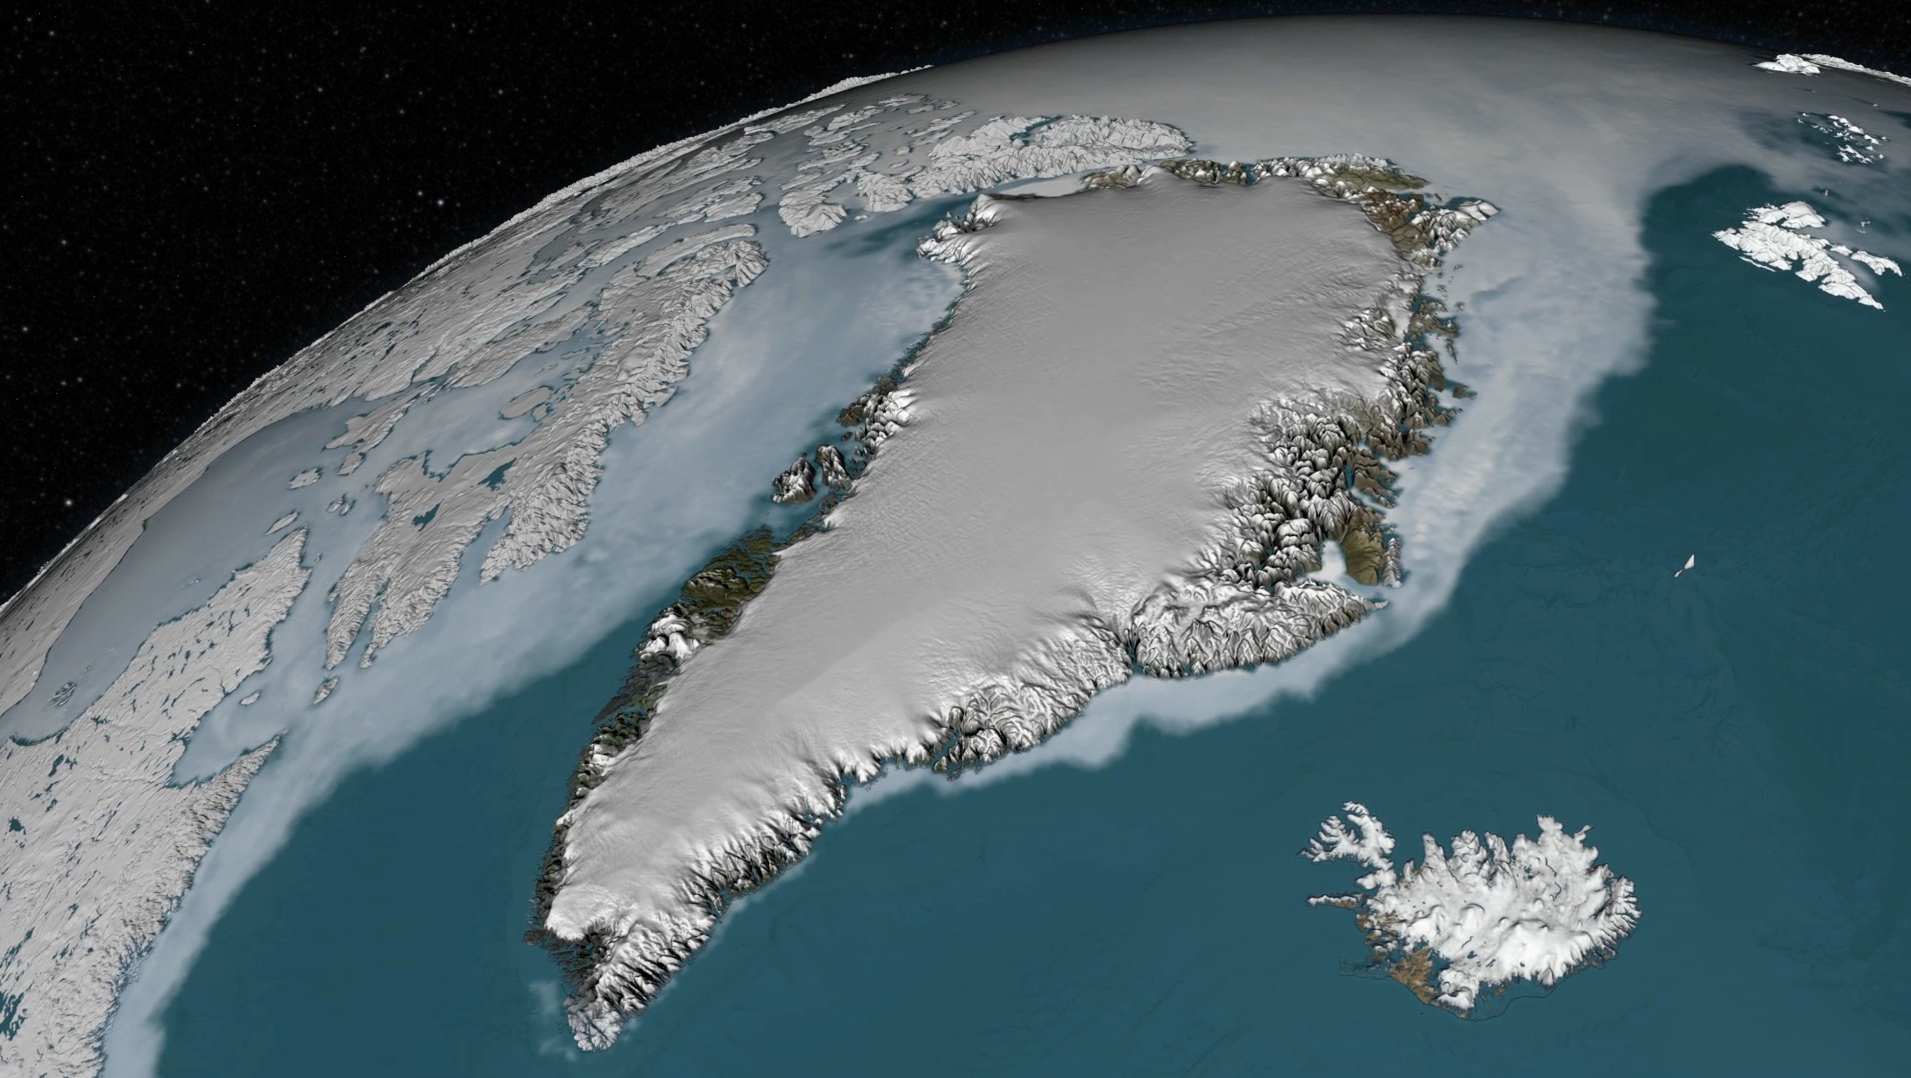
\includegraphics[height=\paperheight,width=\paperwidth]{nasa-mapping-greenland-ice-sheet}};}
} 

\begin{frame}[plain]
  \textbf{The increase in mass loss is roughly equally split between changes in}
  \begin{columns}[c]
    \begin{column}{.3\linewidth}
      \begin{figure}
        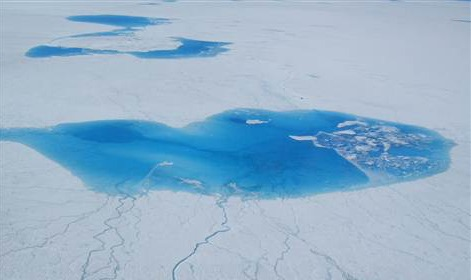
\includegraphics[width=\linewidth]{gris-melt-ponds}
      \end{figure}
    \end{column}
    \begin{column}{.3\linewidth}
      \textbf{surface mass balance}
    \end{column}
  \end{columns}
  \begin{columns}[c]
    \begin{column}{.3\linewidth}
      \begin{figure}
        \includegraphics<1>[width=\linewidth]{storeglacier}
      \end{figure}
    \end{column}
    \begin{column}{.3\linewidth}
      \textbf{ice discharge}
    \end{column}
  \end{columns}
  \bigskip
  \textbf{What does that mean?}
  \note[item]{}
\end{frame}


\setbeamertemplate{background canvas}
{
%
} 


\begin{frame}{How an ice sheet loses mass}
  \begin{figure}
    \includegraphics[width=.96\textwidth]{ice-sheet-cartoon}
  \end{figure}
  \begin{itemize}
    \item before the mid-90s mass loss was dominated by surface mass balance
  \end{itemize}
  \note[item]{explain surface melt, ice discharge/calving, and basal melt}
  \note[item]{snow accumulates in the colder, higher altitude areas in the interior}
  \note[item]{turns into ice}
  \note[item]{and starts to flow downhill towards the coast}
  \note[item]{near the coast, surface melting can occur in the summer}
  \note[item]{but also some ice is dumped directly into the ocean}
  \note[item]{before the mid-90s mass loss was dominated by surface mass balance (80-90\%)}
  \note[item]{contribution of ice discharge was modest (10--20\%)}
  \note[item]{explaining in more detail in the next slide}

\end{frame}


\setbeamertemplate{background canvas}
  {
     \tikz{\node[inner sep=0pt,opacity=.75] {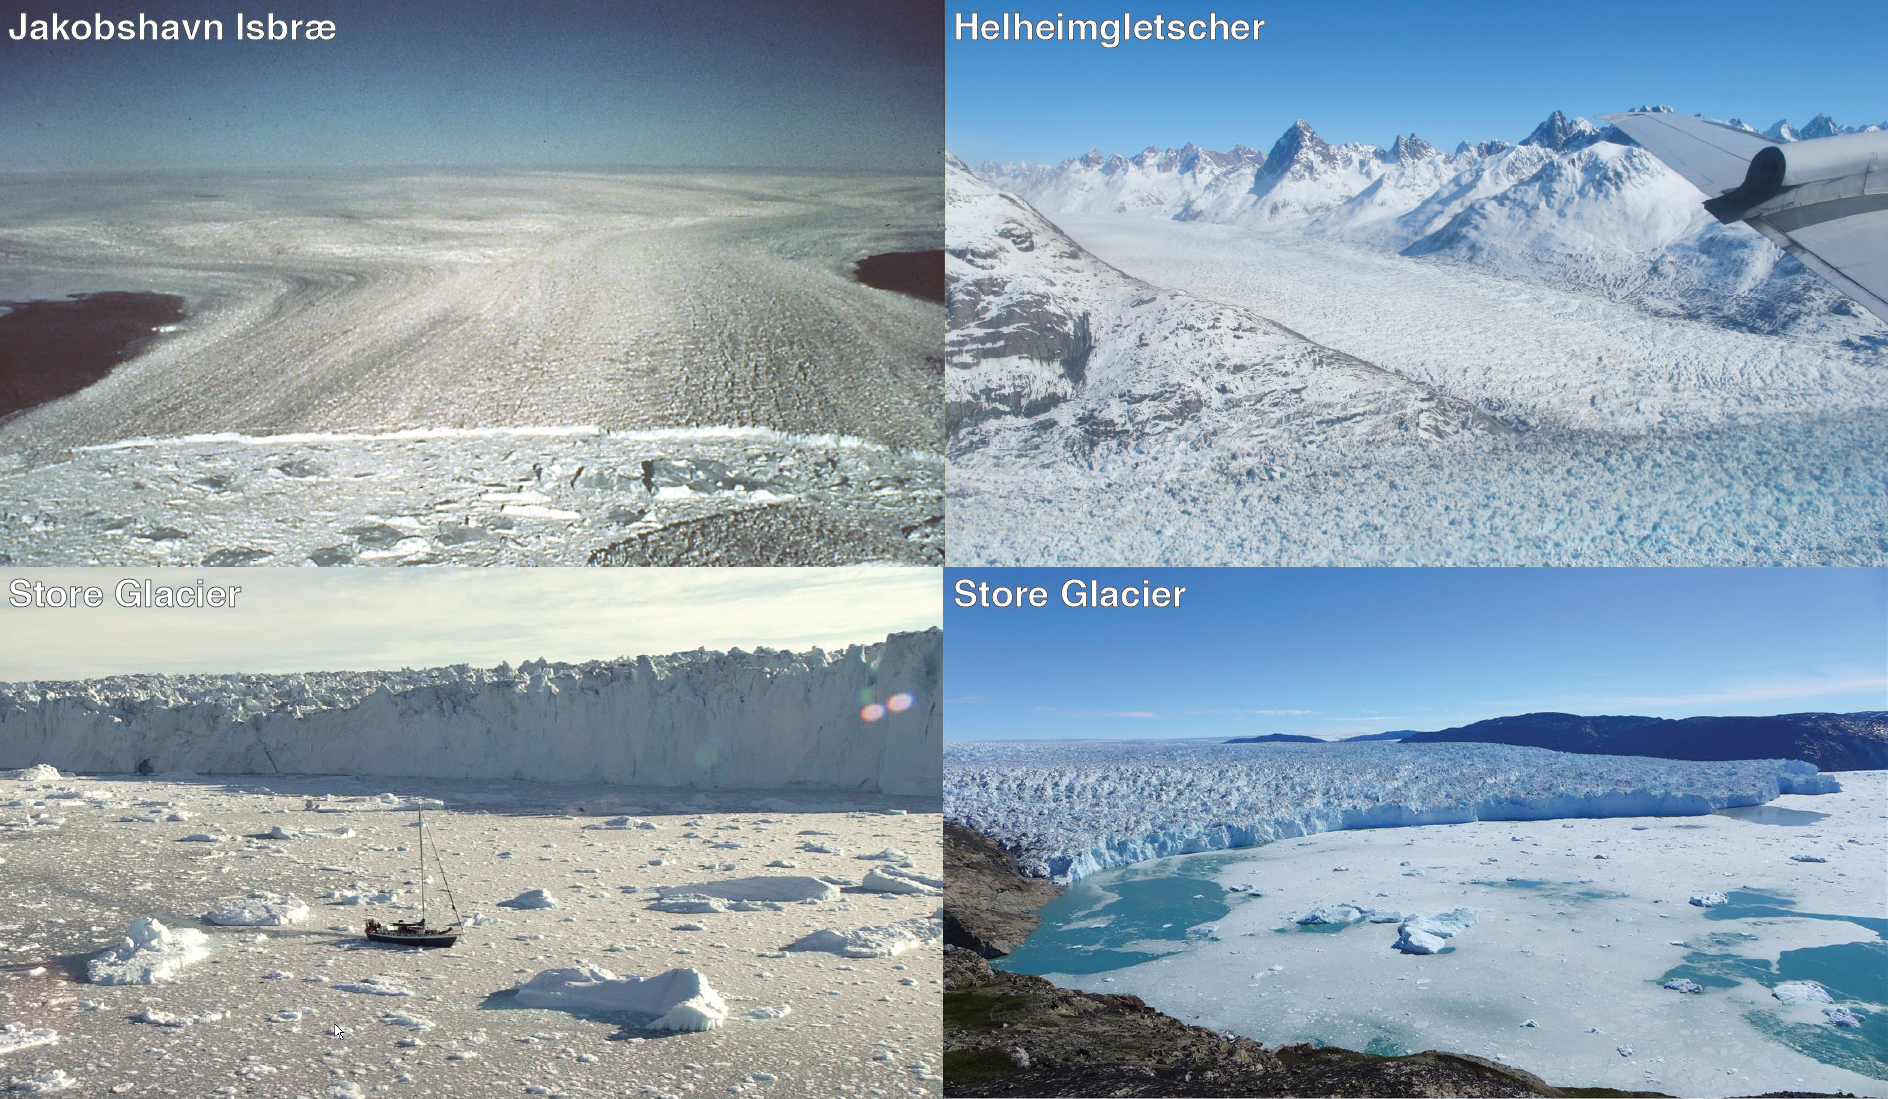
\includegraphics[height=\paperheight,width=\paperwidth]{outlet-glacier-collage-01}};}
}

\begin{frame}[plain]
  \textbf{In Greenland}
    \begin{itemize}
    \item ice discharge to the ocean occurs through 200+ ``outlet glaciers''
    \item outlet glaciers are flowing fast ($>$200\,m/yr), are controlled by bedrock geometry, and terminate in narrow fjords ($\sim <$10\,km wide)
    \end{itemize}
    \note[item]{outlet glaciers look pretty spectacular}
\end{frame}
 

\setbeamertemplate{background canvas}
  {
     \tikz{\node[inner sep=0pt,opacity=1] {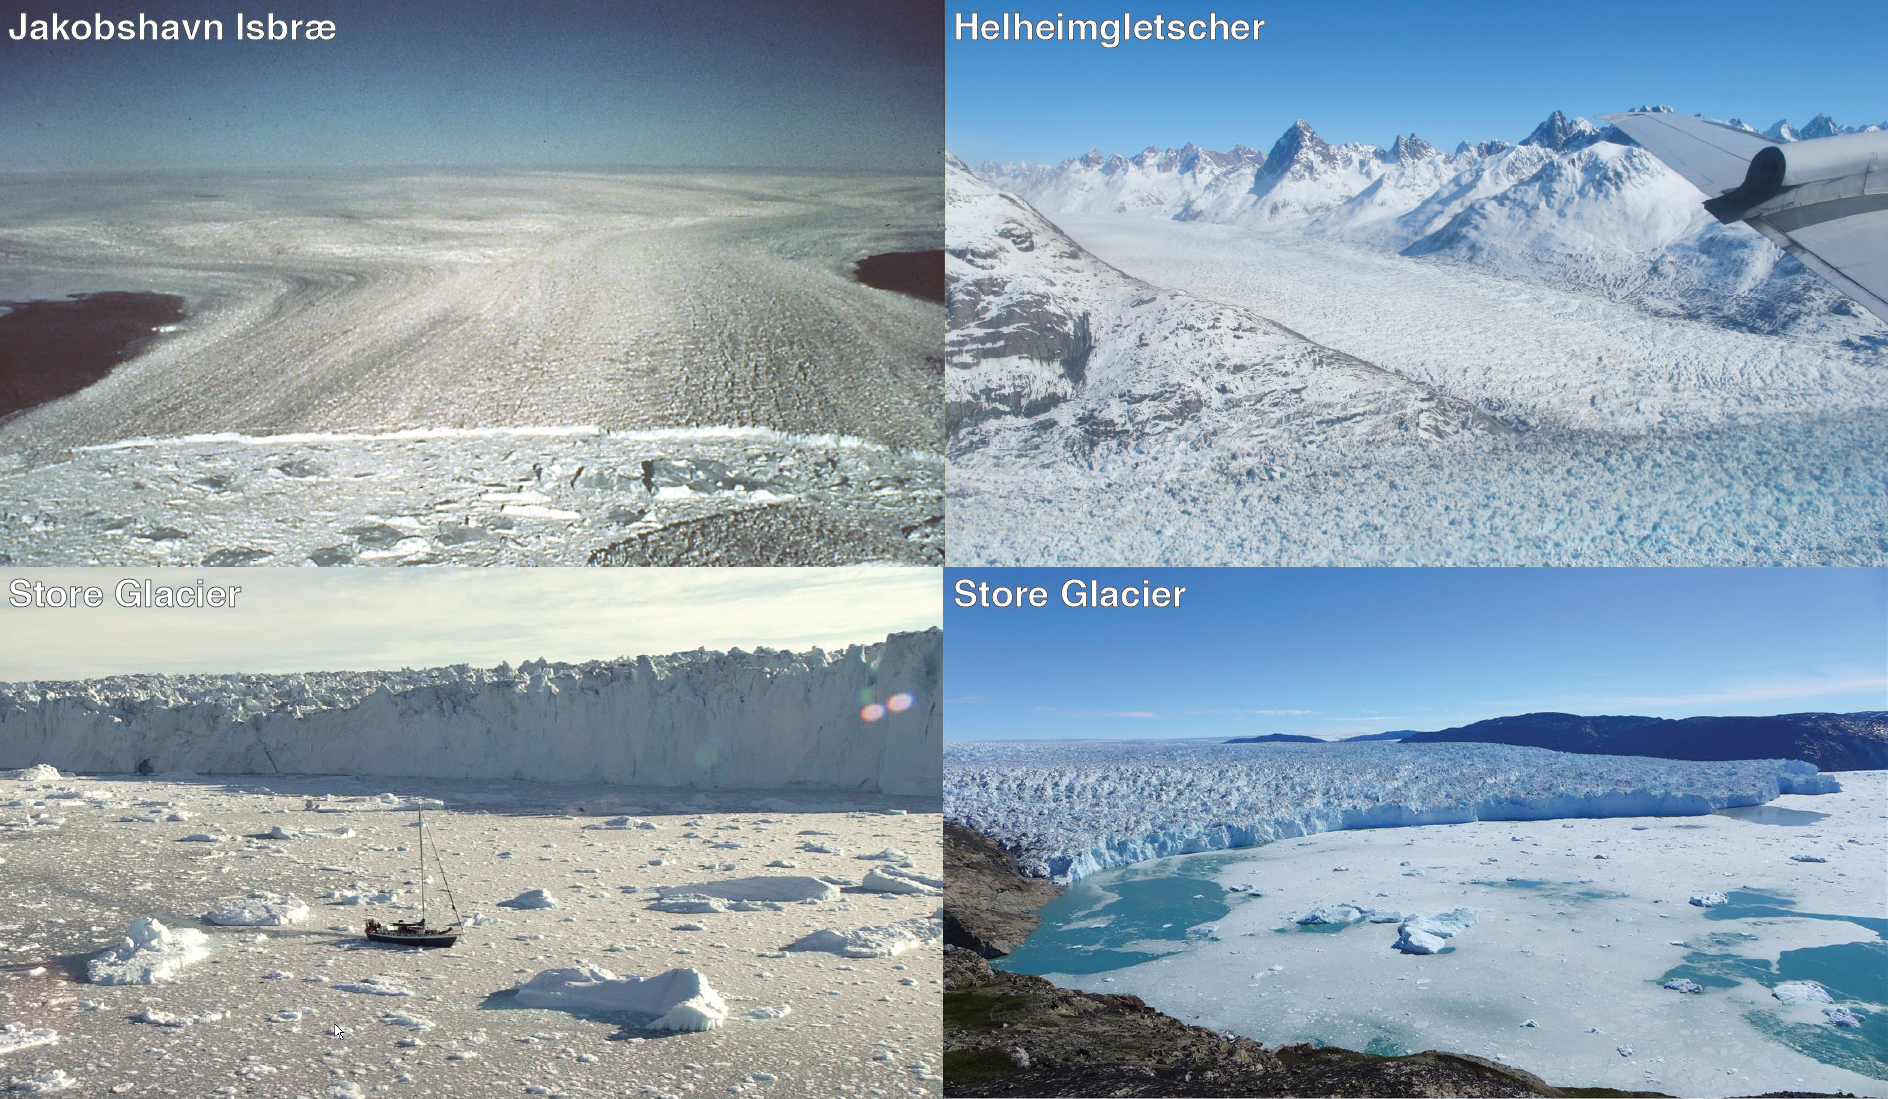
\includegraphics[height=\paperheight,width=\paperwidth]{outlet-glacier-collage-01}};}
}

\begin{frame}[plain]
  \note[item]{some very passionate glaciologists get really close to the terminus in their sailing boats}
\end{frame}


\setbeamertemplate{background canvas}
  {
     \tikz{\node[inner sep=0pt,opacity=1] {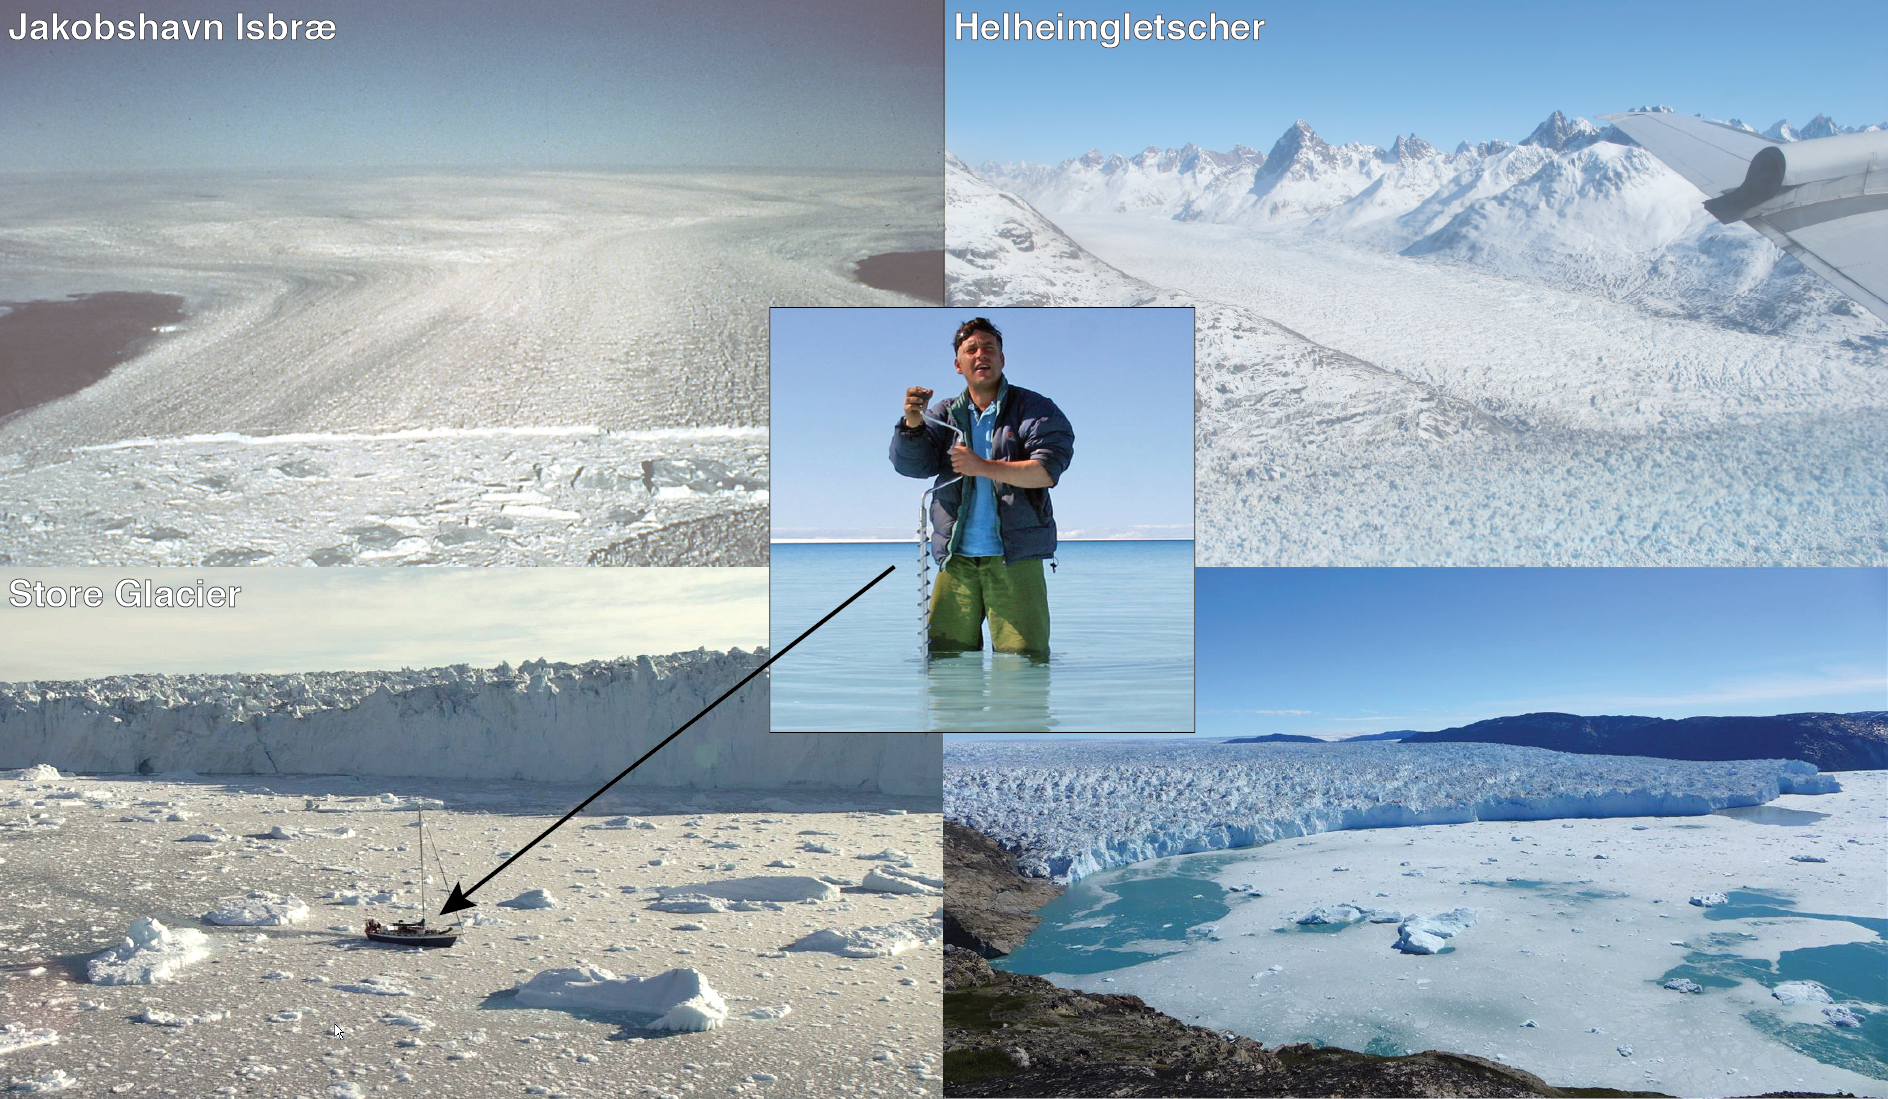
\includegraphics[height=\paperheight,width=\paperwidth]{outlet-glacier-collage-alun-01}};}
}

\begin{frame}[plain]
  \note[item]{some very passionate glaciologists get really close to the terminus in their sailing boats}
\end{frame}



\setbeamertemplate{background canvas}
{
%
} 


\begin{frame}{Jakobshavn Isbr{\ae}, west Greenland}
    \begin{columns}[c]
    \begin{column}{.50\linewidth}
      \begin{figure}
        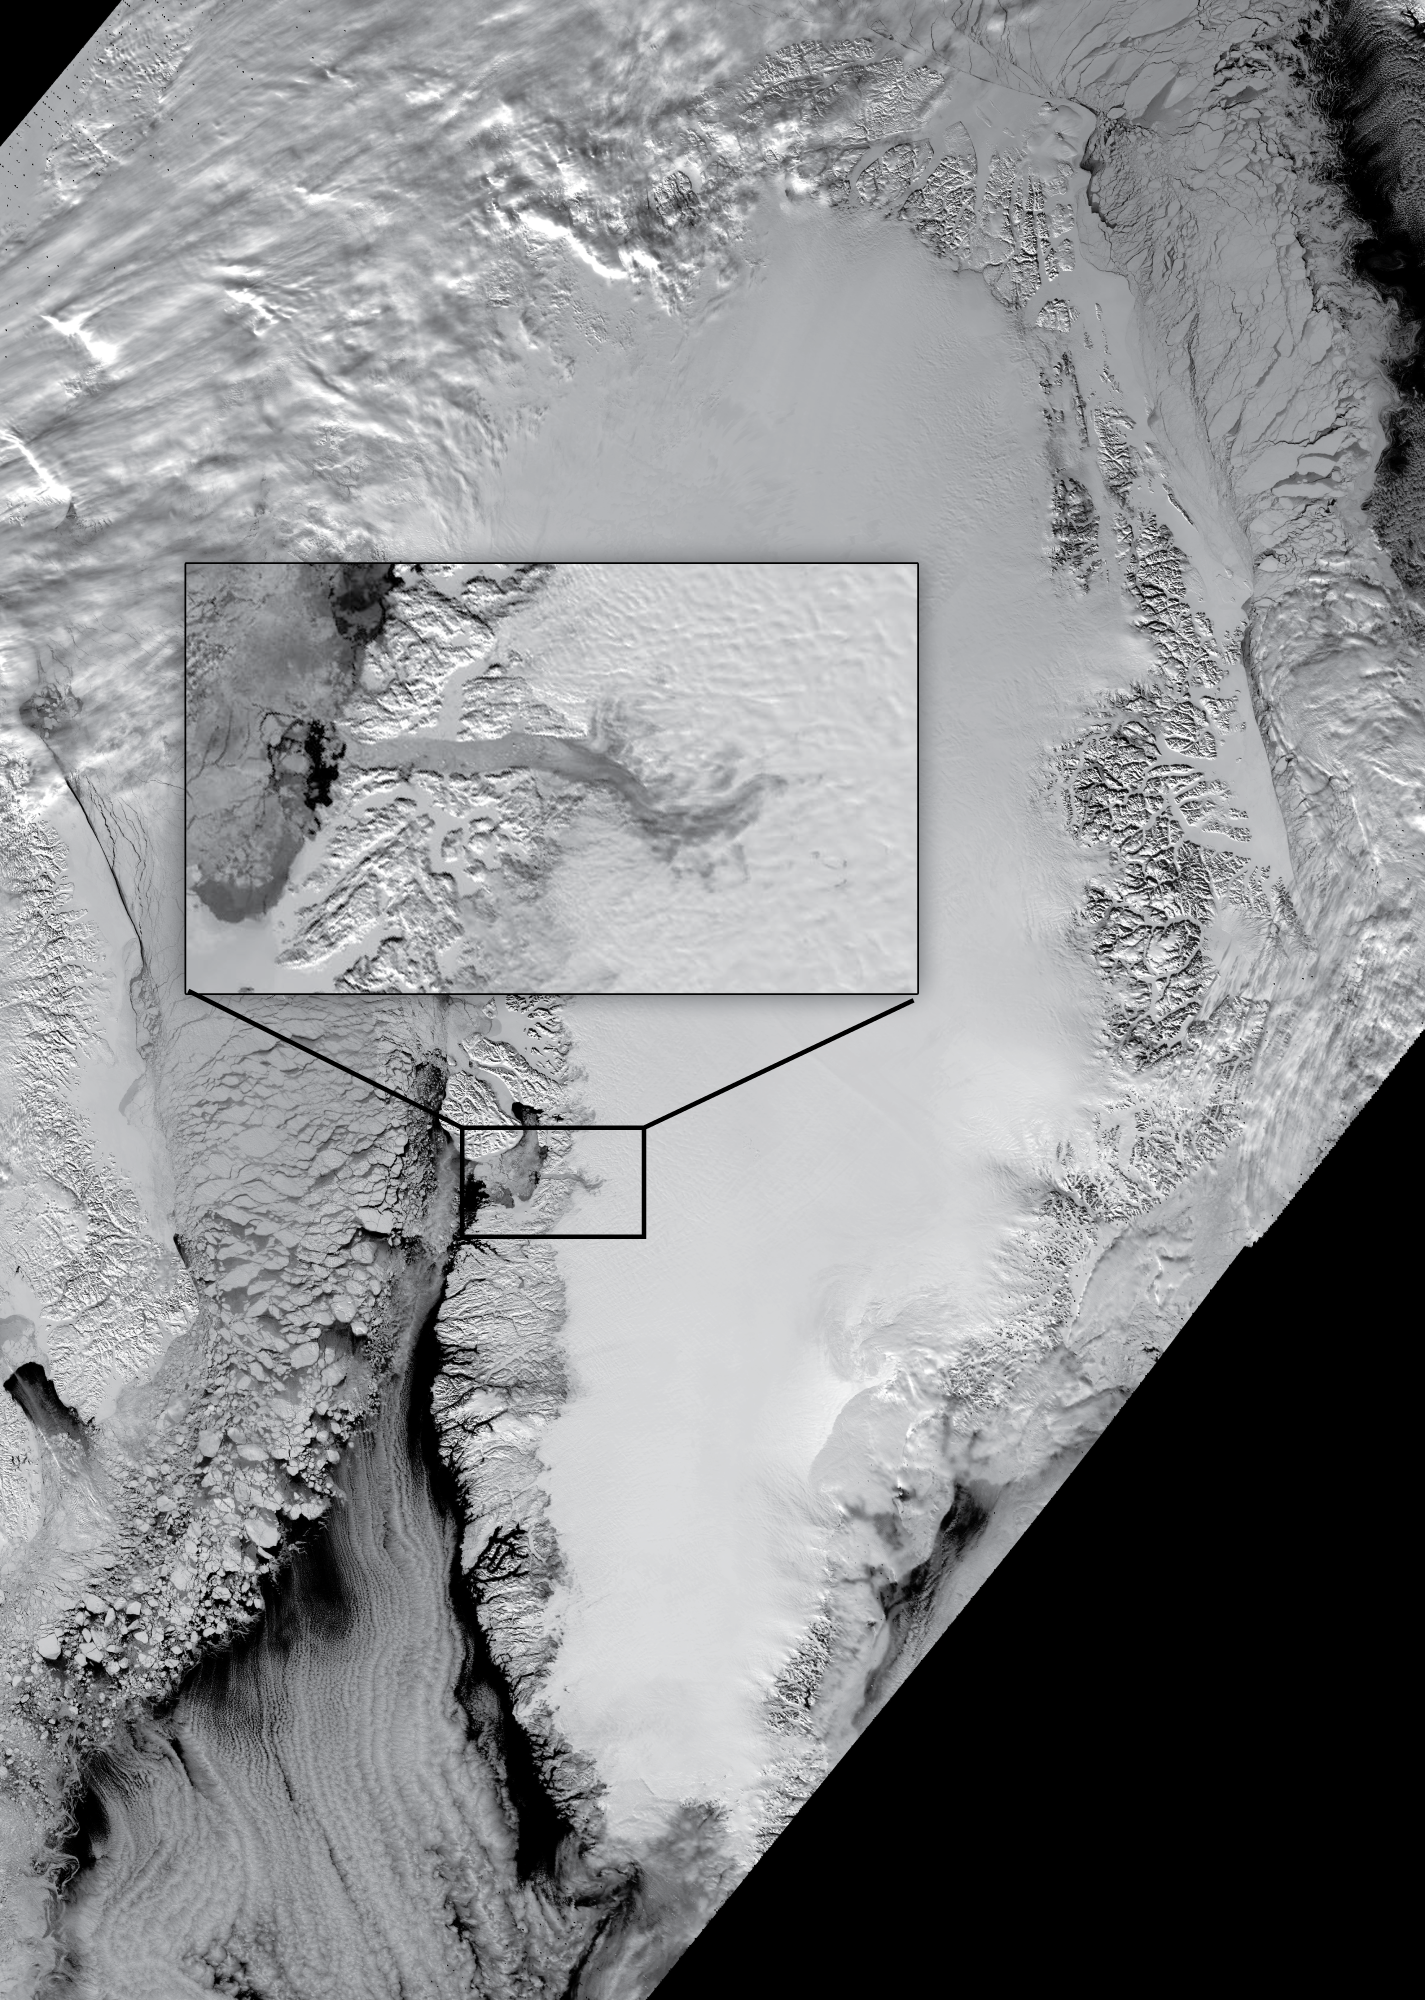
\includegraphics[height=.8\textheight]{MODISGreenlandJakobshavn} \\
        \scriptsize{based on MODIS data from M. Fahnestock}
      \end{figure}
    \end{column}
    \begin{column}{.50\linewidth}
      \begin{itemize}
      \item Greenland's biggest and fastest flowing outlet glacier
      \item drains about 7\% of the entire ice sheet
      \end{itemize}
    \end{column}
  \end{columns}
  \note[item]{Let's focus on Jakobshavn Isbr{\ae}}
  \note[item]{Greenland's biggest and fastest flowing outlet glacier}
  \note[item]{drains about 7\% of the entire ice sheet}
\end{frame}


\begin{frame}{A short history}
 \begin{figure}
    \includegraphics[width=\textwidth]{Jakobshavn_groundline_retreat} \\
  \end{figure}
  \note[item]{My colleagues Will Harrison and late Keith Echelmeyer investigated Jakobshavn in the mid-80s}
  \note[item]{at that time JIB had a $\sim$10\,km long floating tongue}
  \note[item]{they found high flow speeds}
  \note[item]{relatively steady behavior}
  \note[item]{in 1997, the glacier suddenly switched from slow thickening to rapid thinning}
  \note[item]{caused by an increase in subsurface ocean temperature from 1.7degC in 1995 to 3.3degC in 1998, leading to increased melting}
  \note[item]{In summer 1998 the first major increase in surface velocity was seen}
  \note[item]{first departure from the normal pattern of frontal positions 1998}
  \note[item]{retreat of the ice front started around 2001}
\end{frame}


\begin{frame}{Frontal retreat 1990--2005}
 \begin{figure}
    \includegraphics<1>[width=\textwidth]{jib-front-1990}
    \includegraphics<2>[width=\textwidth]{jib-front-1990-floating}
    \includegraphics<3>[width=\textwidth]{jib-front-2005}
    \includegraphics<4>[width=\textwidth]{jib-front-1990-2005-change}
    \includegraphics<5>[width=\textwidth]{jib-front-1990-2005-plug}
  \end{figure}
  \note[item]{the loss of the floating tongue is what I'm calling pulling the plug}
  \note[item]{exact timing of the break-up remains elusive due to poor satellite coverage at that time}
\end{frame}


\begin{frame}{When you pull the plug: speed-up 1992-2000}
  \begin{itemize}
    \item almost doubled its flow speed between the 1992 and 2000
    \item slow but steady increase since then
  \end{itemize}
  \begin{figure}
    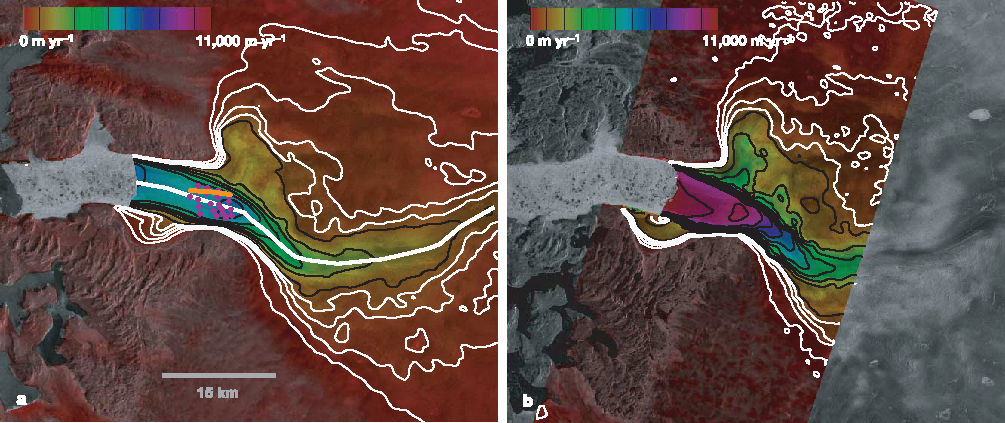
\includegraphics[width=\textwidth]{Joughin2004Fig2} \\
    \footnotesize{Joughin et al. (2004)}
  \end{figure}
  \note[item]{illustration of the speed up}
\end{frame}


\setbeamertemplate{background canvas}
  {
     \tikz{\node[inner sep=0pt,opacity=0.8] {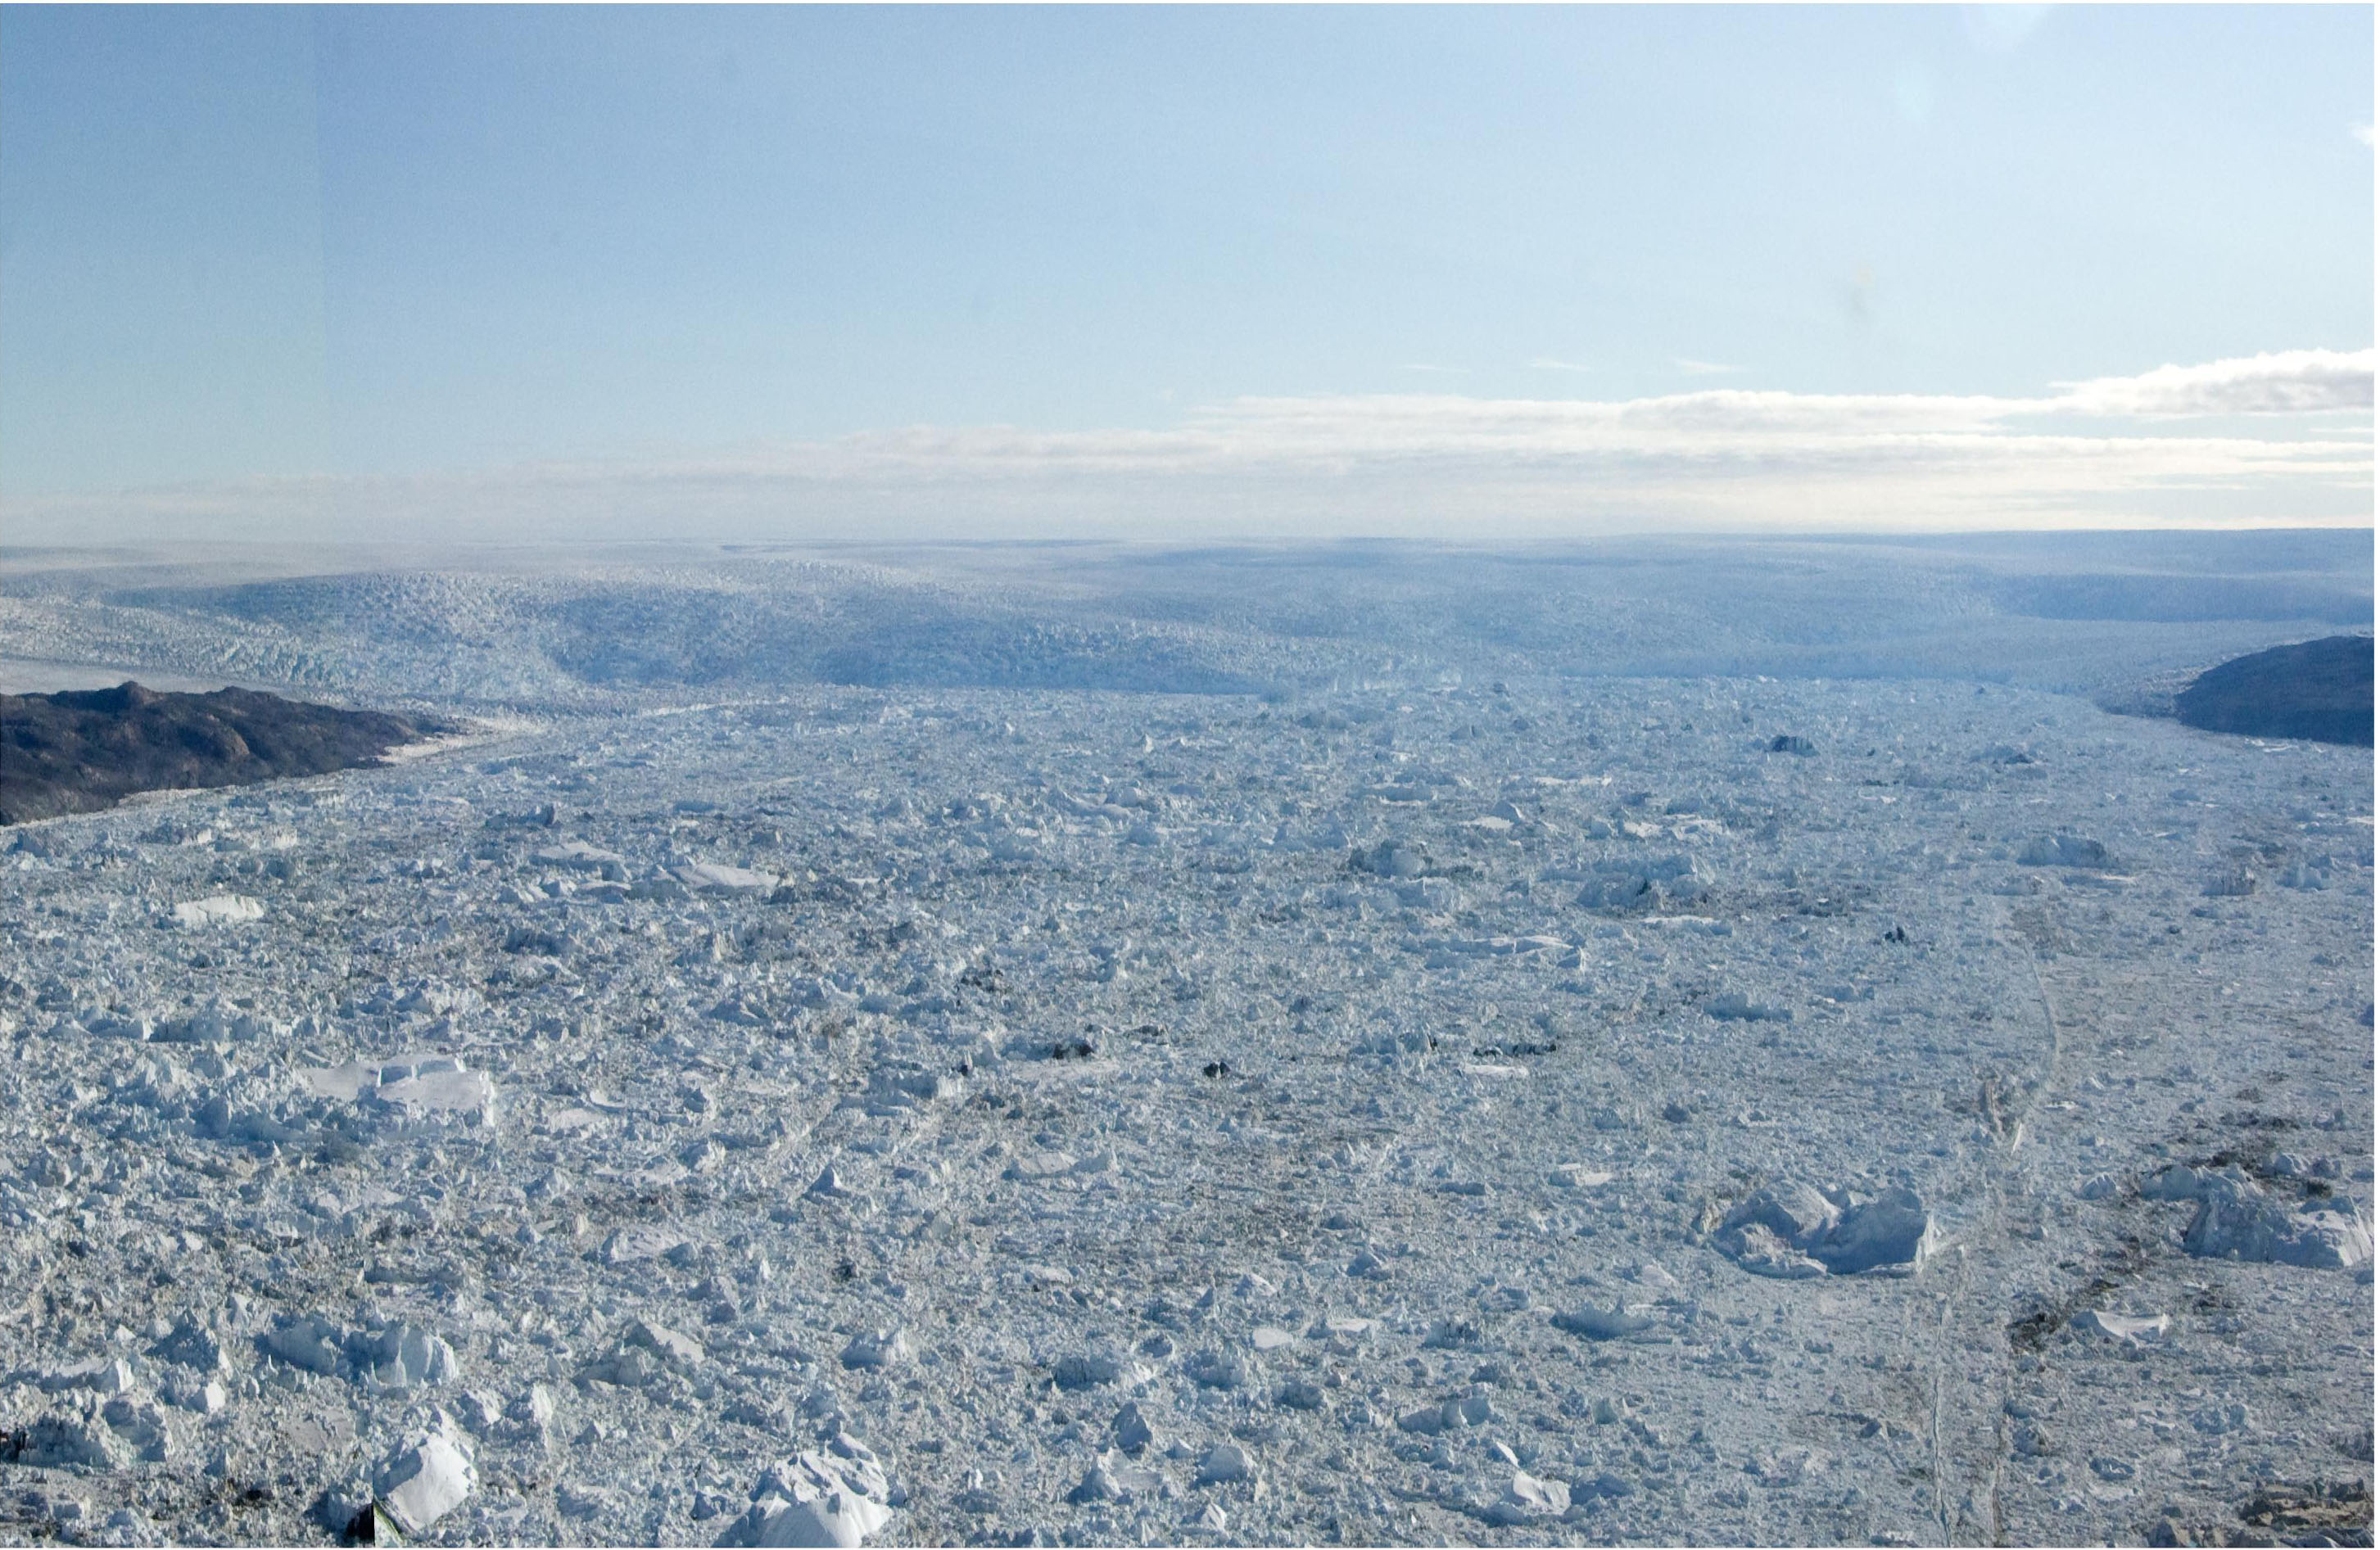
\includegraphics[height=\paperheight,width=\paperwidth]{jakobshavn-2007}};}
}


\begin{frame}{When you pull the plug: changes in ice discharge 2000--2010}
  \begin{itemize}
  \item increase in discharge from 40\,Gt/yr in 2000 to $\sim$60\,Gt/yr in 2010
  \item compared to $\sim$75\,Gt/yr total mass loss from all Alaskan glaciers (as far as I know there are no glaciers in South Korea)
  \end{itemize}
  \note[item]{illustration of the speed up}
\end{frame}


\setbeamertemplate{background canvas}
{
%
} 

\begin{frame}{When you pull the plug: surface elevation changes 1985-2007}

  \begin{figure}
    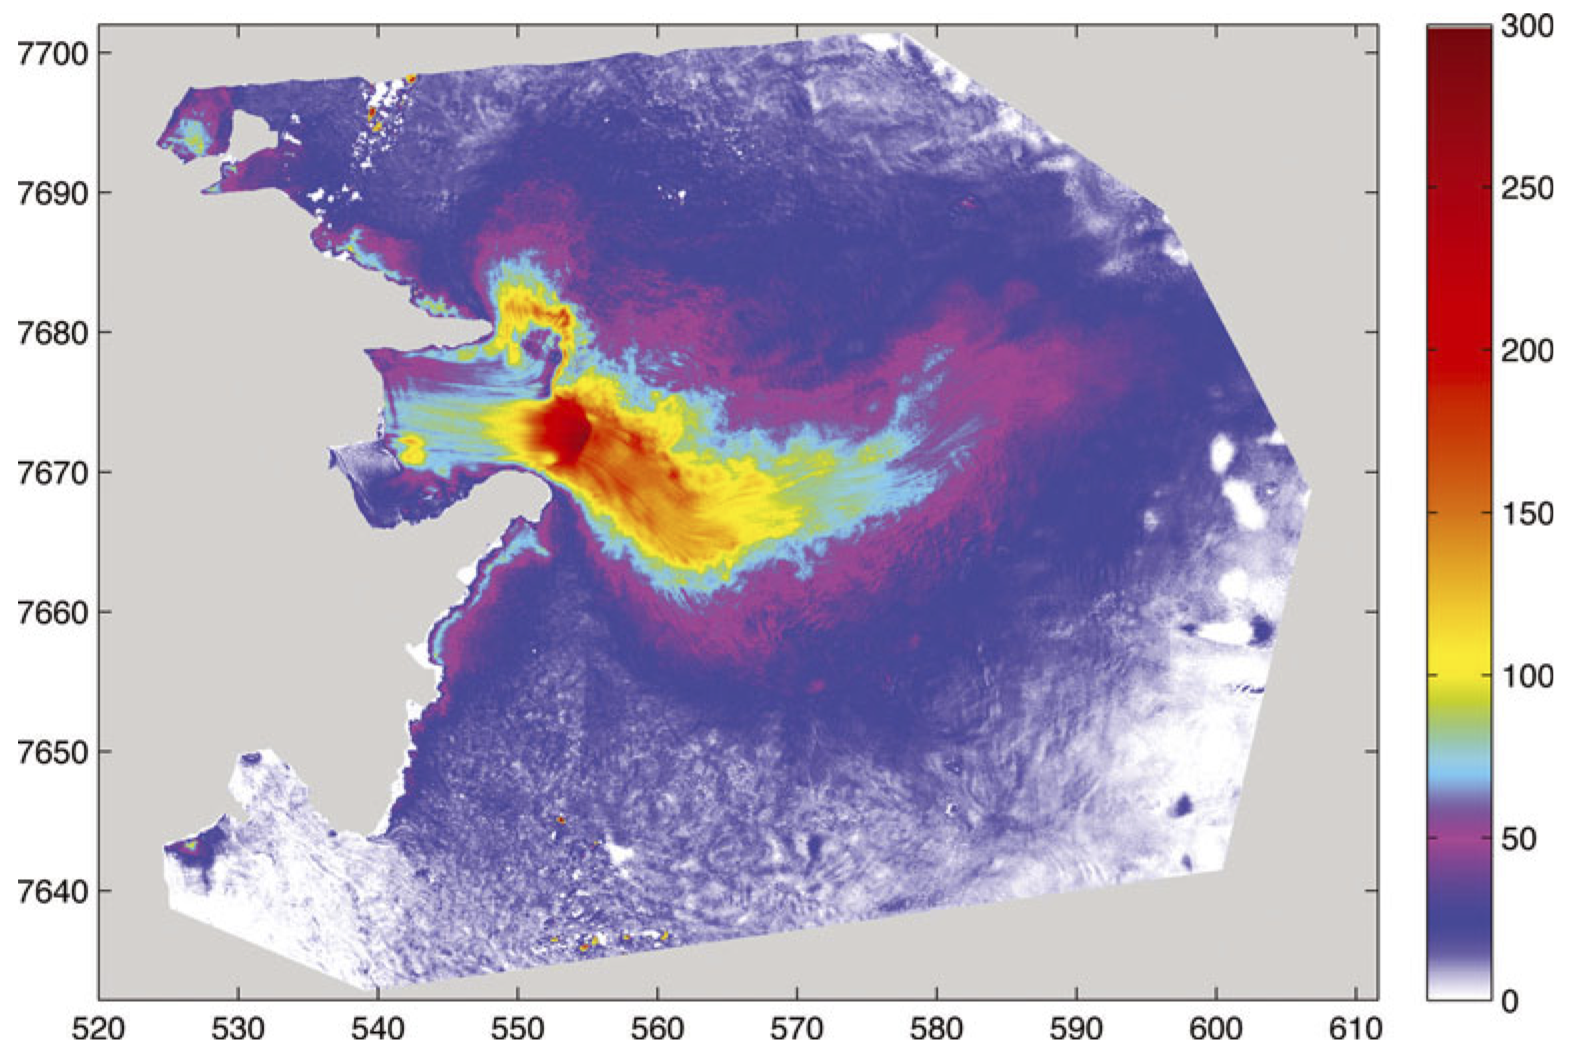
\includegraphics[width=.8\textwidth]{jib-obs-surface-diff-motyka} \\
    \footnotesize{Motyka, Fahnestock, Truffer (2010)}
  \end{figure}
  \note[item]{as a consequence of the increased discharge, the ice surface is drawing down near the glacier terminus}
\end{frame}


\begin{frame}{How can we reconcile/understand these changes?}
 \begin{figure}
    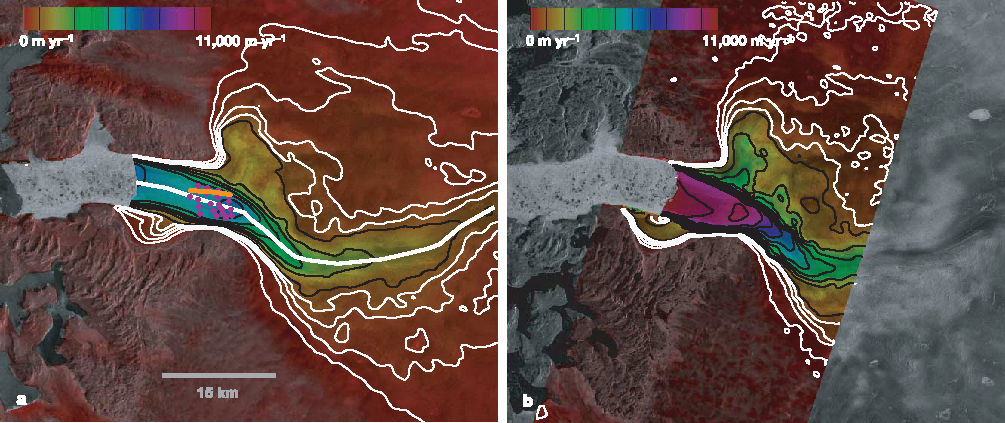
\includegraphics[height=4.15cm]{Joughin2004Fig2} \\
    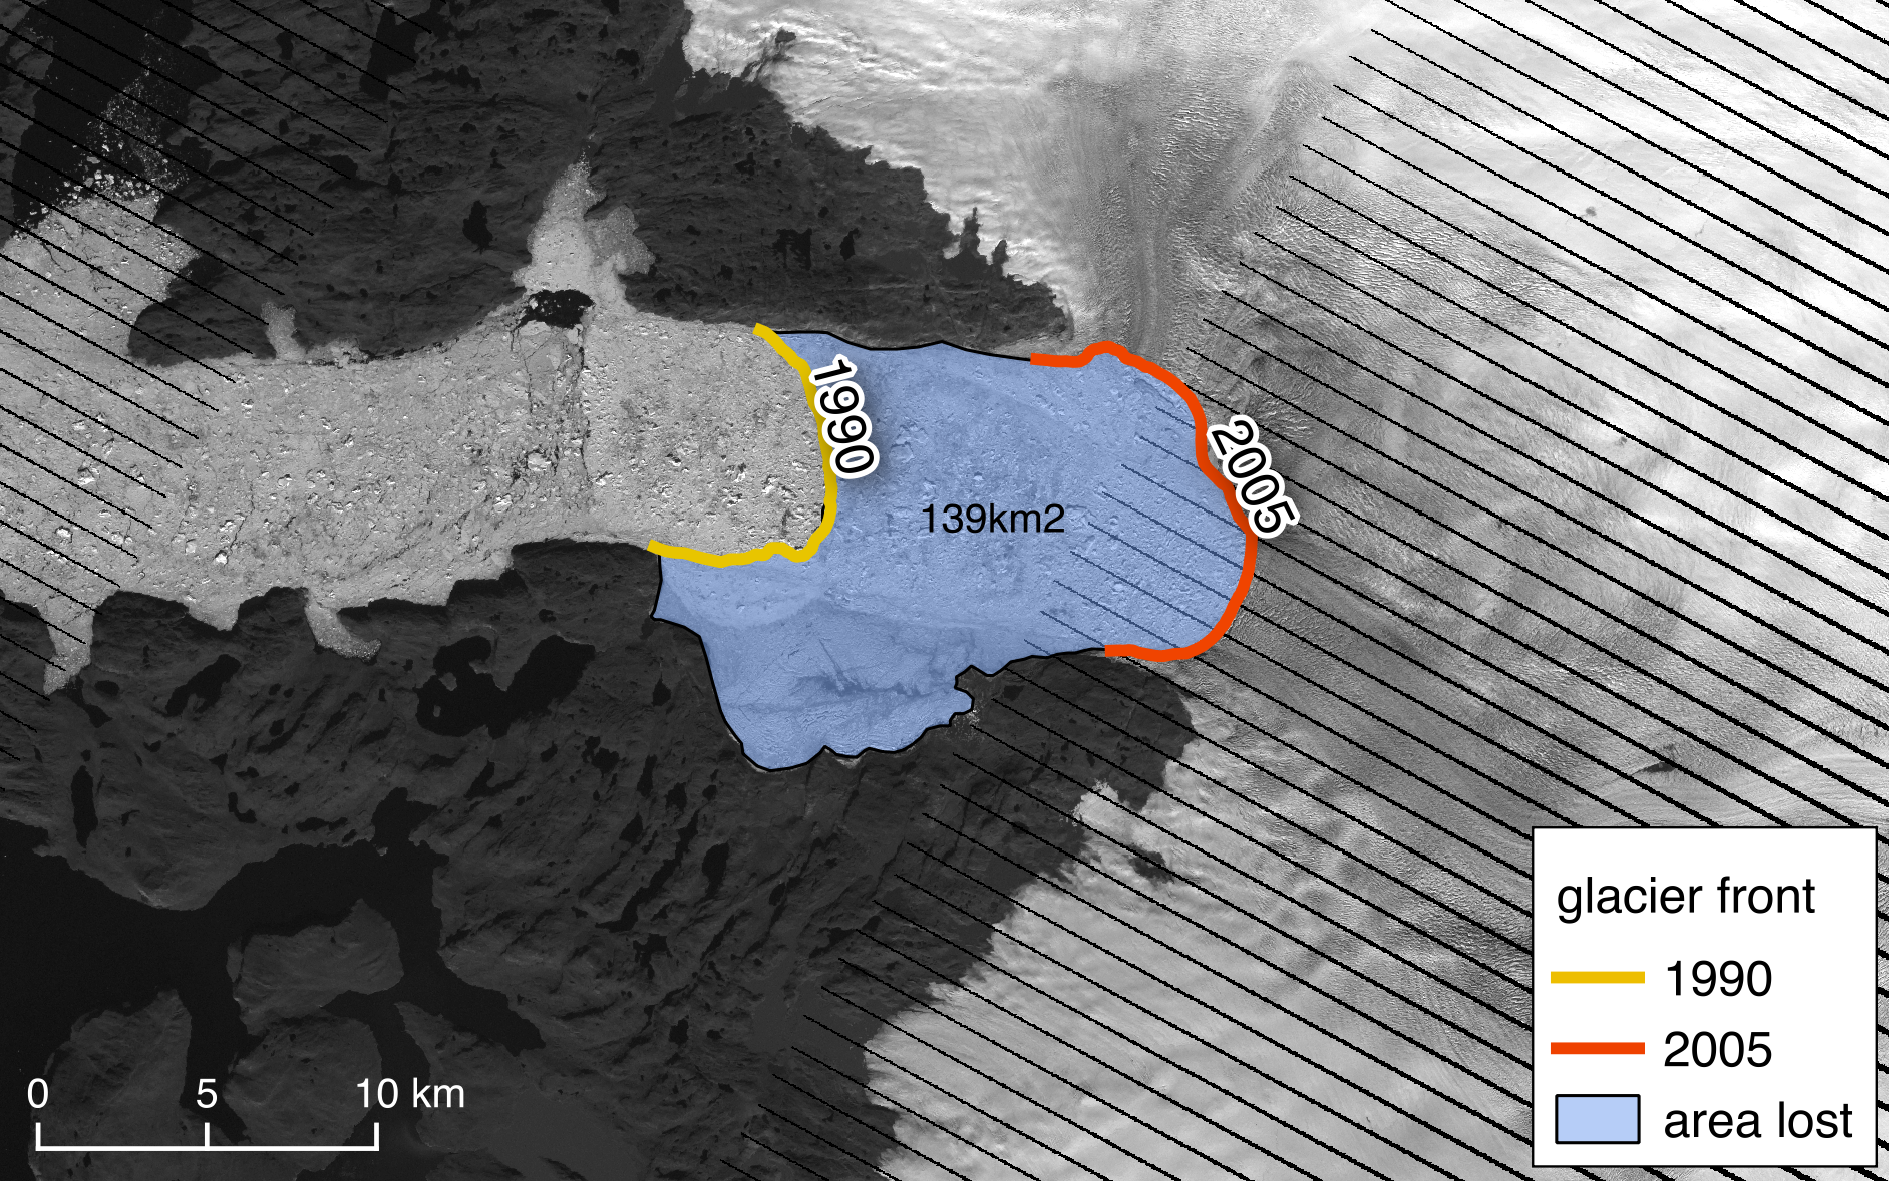
\includegraphics[height=3.20cm]{jib-front-1990-2005-change}
    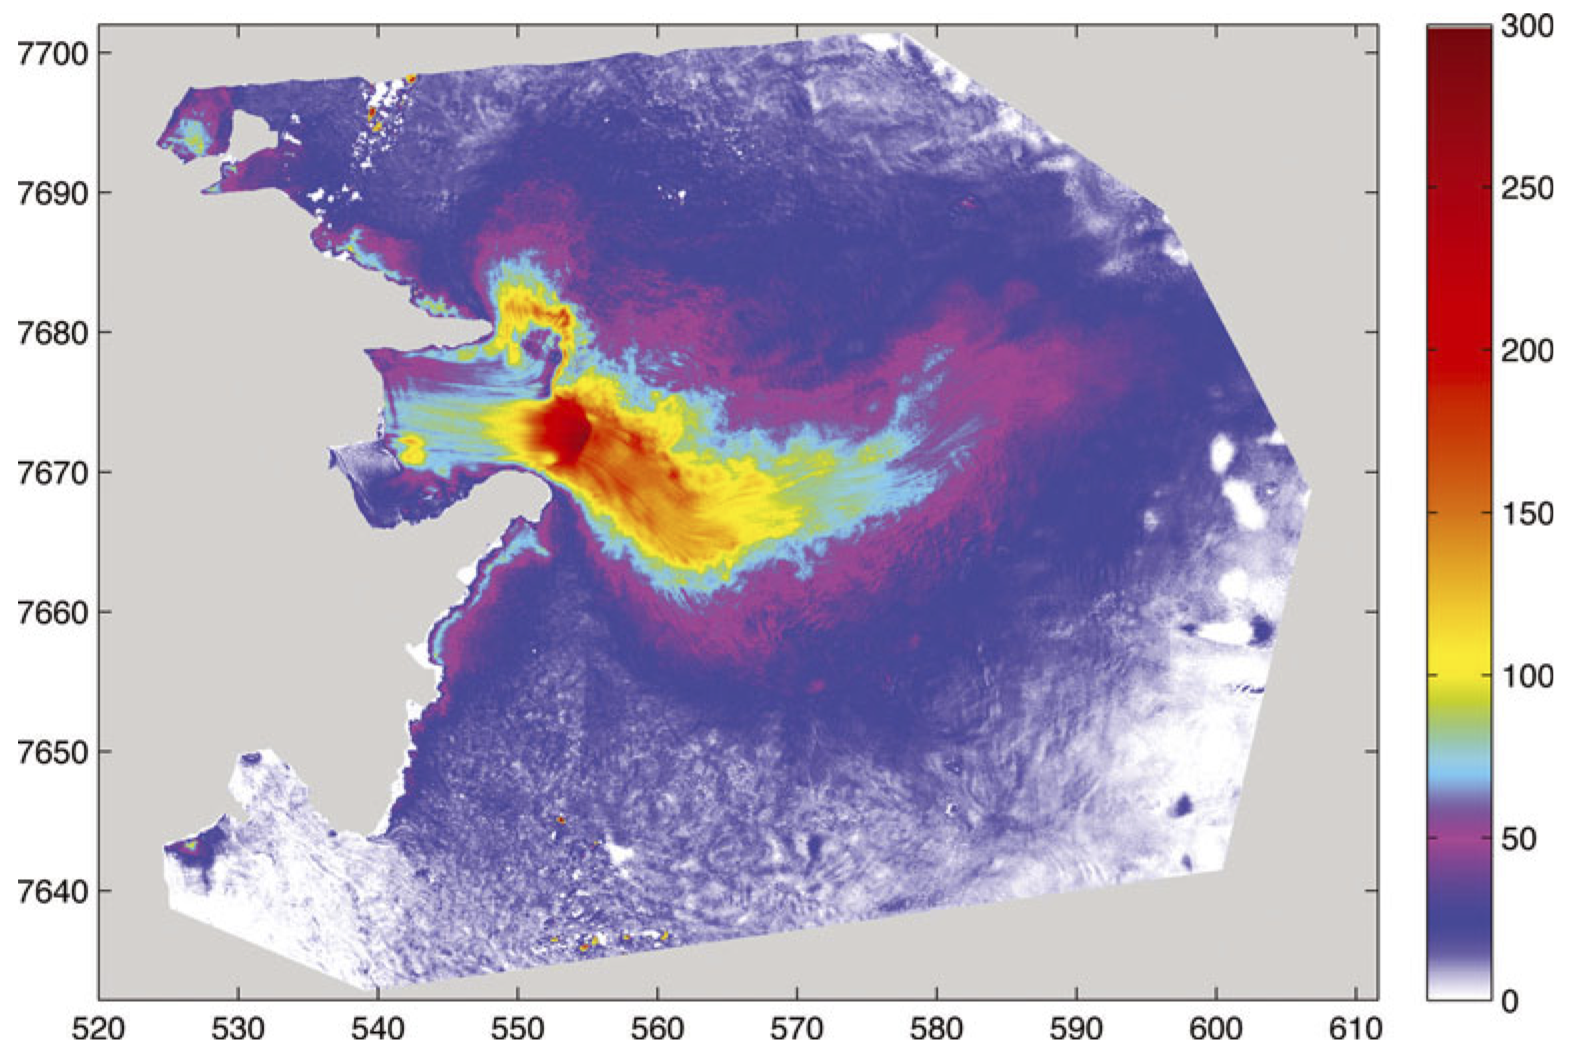
\includegraphics[height=3.20cm]{jib-obs-surface-diff-motyka}
  \end{figure}
\end{frame}


\begin{frame}{Answer: use an ice sheet model}
  \begin{figure}
    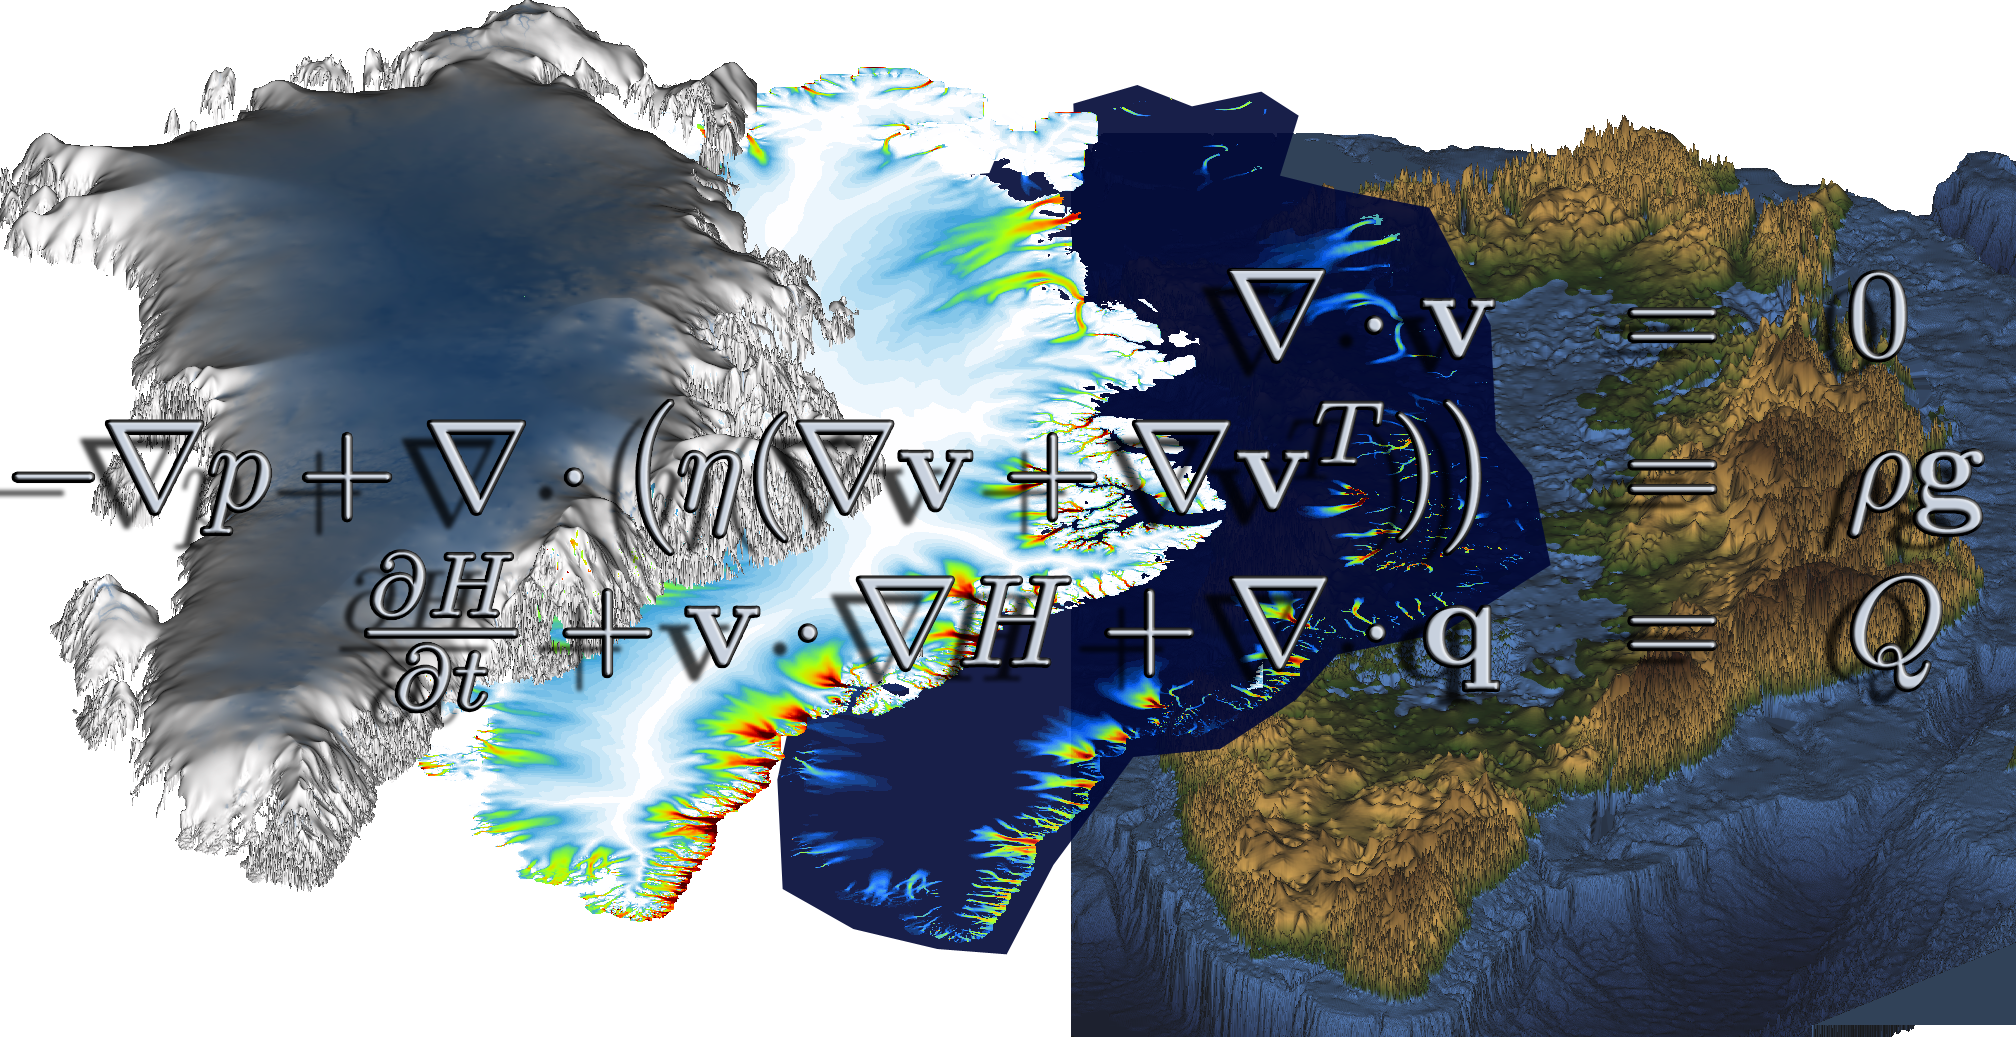
\includegraphics[width=8cm]{grn_system_eqns}
  \end{figure}
  \begin{columns}[c]
    \begin{column}{.40\linewidth}
      \begin{itemize}
      \item ice dynamics (mass and momentum balance)
      \item thermodynamics (energy balance)
      \item surface processes
      \end{itemize}
    \end{column}
    \begin{column}{.55\linewidth}
      \begin{itemize}
      \item boundary conditions
      \item hydrology
      \item ice-ocean interaction (e.g. calving, frontal melting)
      \end{itemize}
    \end{column}
  \end{columns}
  \note[item]{An ice sheet model solves numerical approximations to the balance equations of mass, momentum}
  \note[item]{Ice flow is governed by Stokes equations with a power-law rheology}
  \note[item]{Because the viscosity of ice strongly depends on the thermal state, we also need to solve an energy balance equation}
  \note[item]{This makes the problem thermomechanically-coupled.}
\end{frame}


\begin{frame}{Why ice sheet modeling is easy}
  \begin{columns}[c]
    \begin{column}{.28\linewidth}
      \begin{figure}
        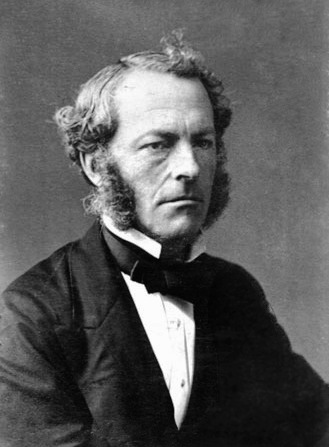
\includegraphics[width=\linewidth]{ggstokes}
        \\ \scriptsize{G.~G.~Stokes}
      \end{figure}
    \end{column}
    \begin{column}{.67\linewidth}
      \begin{itemize}[<+- | alert@+>]
      \item composed of a single, largely homogeneous material
      \item flow governed by the Stokes equations known since the mid-19th century
      \item flows slowly: we can ignore turbulence, Coriolis and other inertial effects
      \item no density/salinity stratification
      \item most of what makes atmosphere and ocean flow interesting is missing
      \item so what makes the flow of slow, cold, laminar ice interesting?
      \end{itemize}
    \end{column}
  \end{columns}
\end{frame}


\begin{frame}{Why ice sheet modeling is so hard}
    \begin{columns}[c]<1-2>
      \begin{column}{.28\linewidth}
        \begin{figure}
          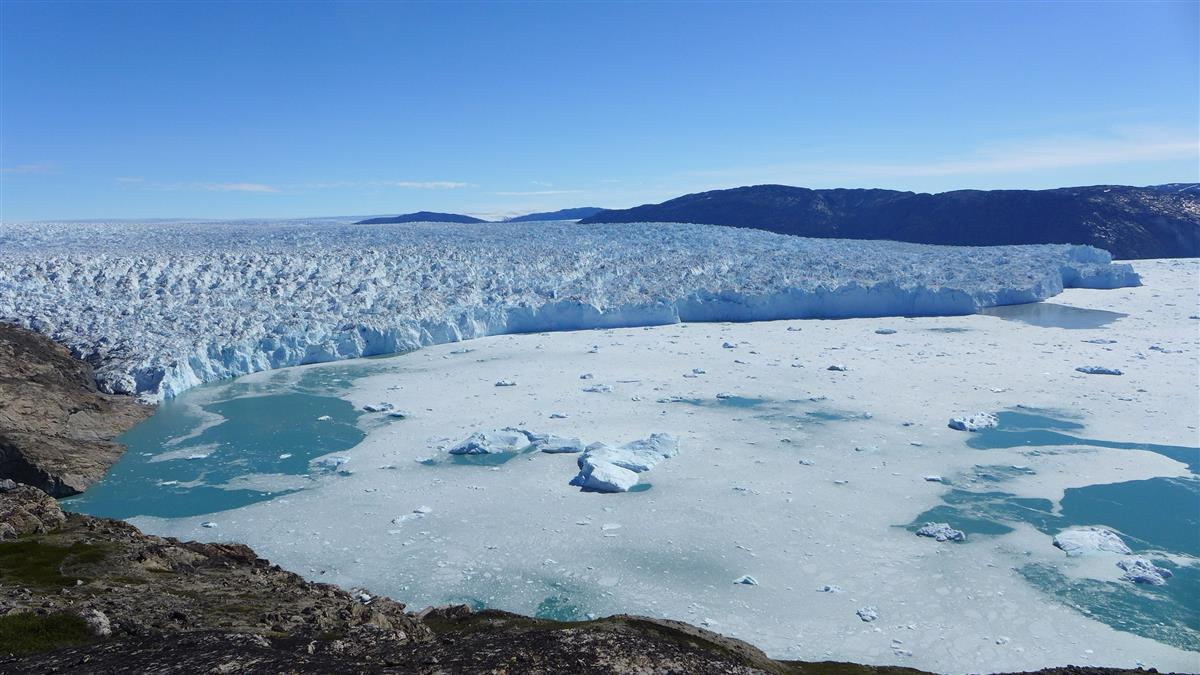
\includegraphics[width=\linewidth]{storeglacier}
        \end{figure}
      \end{column}
      \begin{column}{.67\linewidth}
        \begin{block}{Boundary conditions}
        \begin{itemize}
        \item seaward margin boundary condition
        \item basal boundary condition
        \end{itemize}
      \end{block}
      \end{column}
    \end{columns}
    \begin{columns}[c]<1>
      \begin{column}{.28\linewidth}
        \begin{figure}
          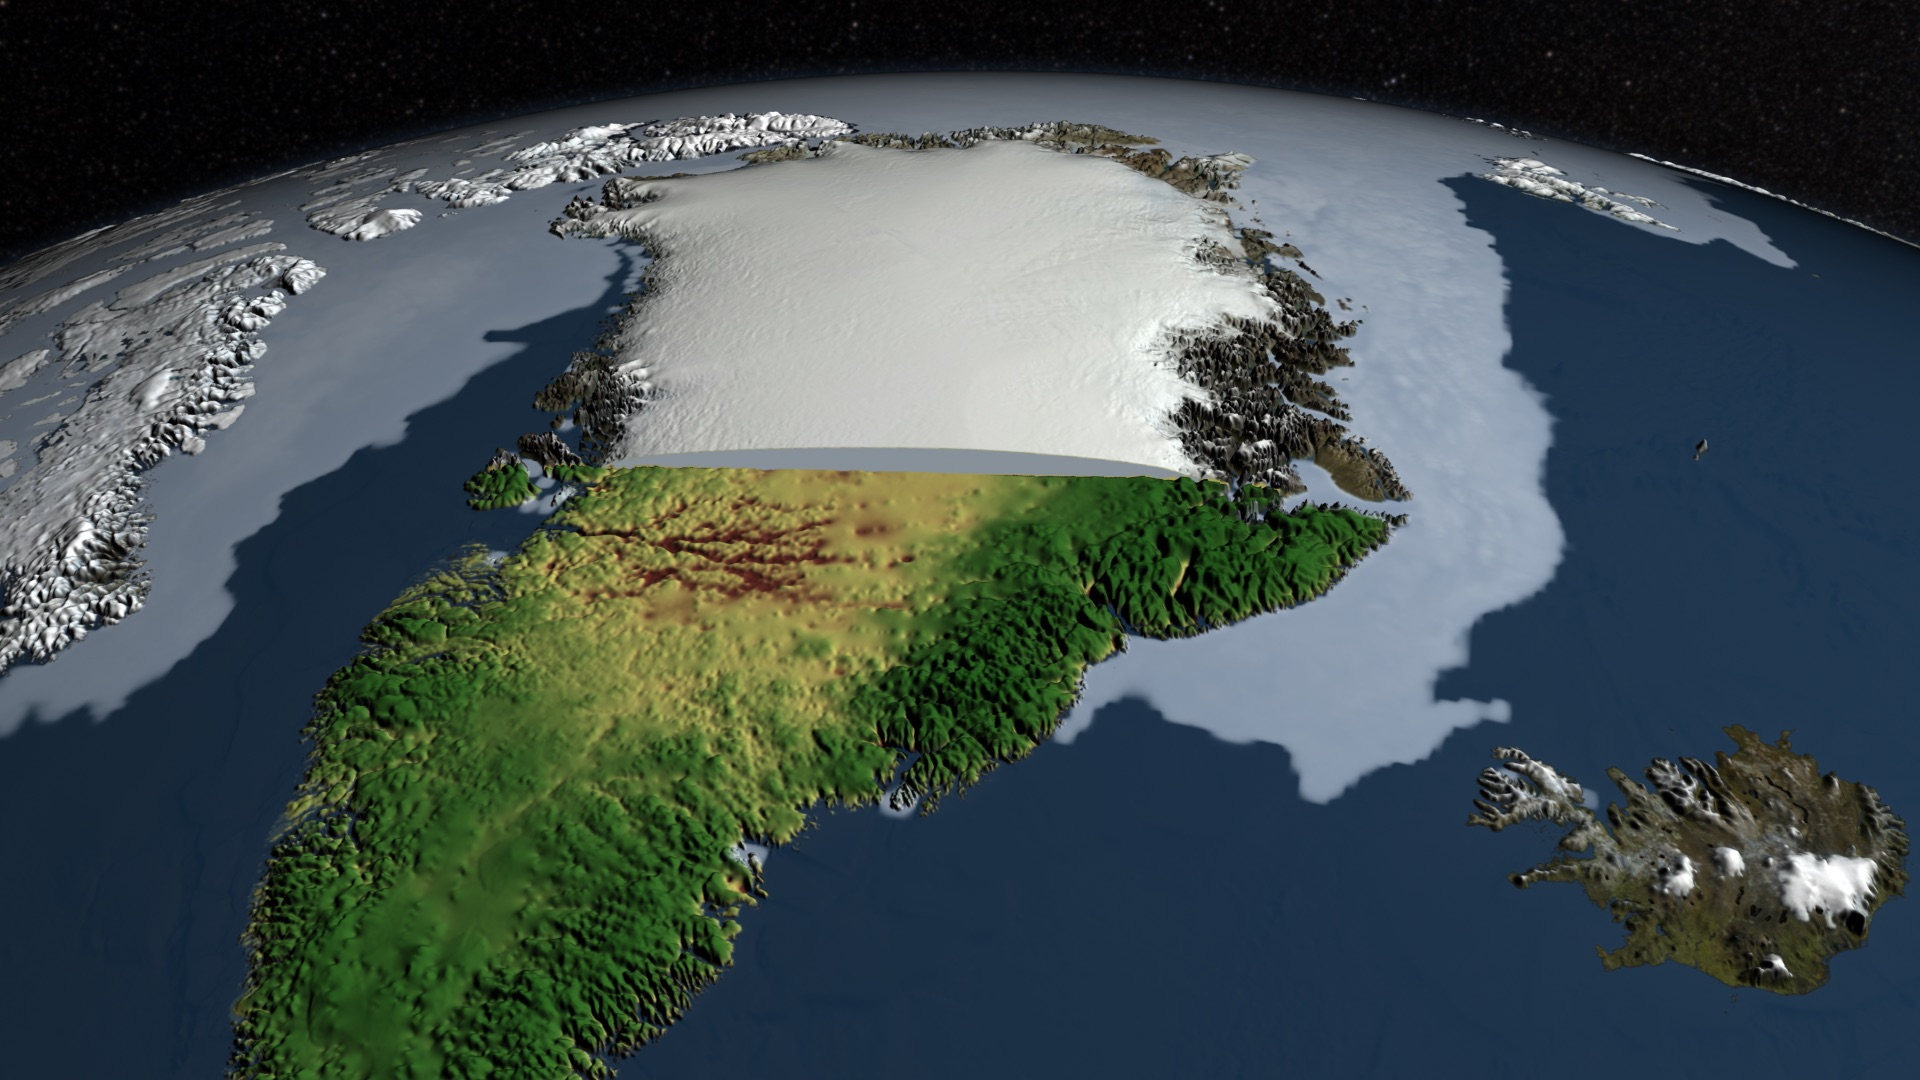
\includegraphics[width=\linewidth]{canale_grande_V05}
        \end{figure}
      \end{column}
      \begin{column}{.67\linewidth}
        \begin{block}{Initial conditions}
        \begin{itemize}
        \item ice thickness / subglacial topography is a first order constraint on ice flow
        \end{itemize}
      \end{block}
      \end{column}
    \end{columns}
    \begin{columns}[c]<1>
      \begin{column}{.3\linewidth}
        \begin{figure}
          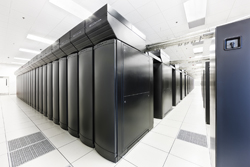
\includegraphics[width=\linewidth]{bw_front_sm}
        \end{figure}
      \end{column}
      \begin{column}{.67\linewidth}
        \begin{block}{Computational costs}
        \begin{itemize}
        \item solving the Stokes equations is computationally very expensive
        \end{itemize}
      \end{block}
      \end{column}
    \end{columns}
\end{frame}


\begin{frame}{Challenge: basal boundary condition}
  \begin{columns}[c]
    \begin{column}{.45\linewidth}
      \begin{figure}
        \scriptsize{basal resistance} \\
        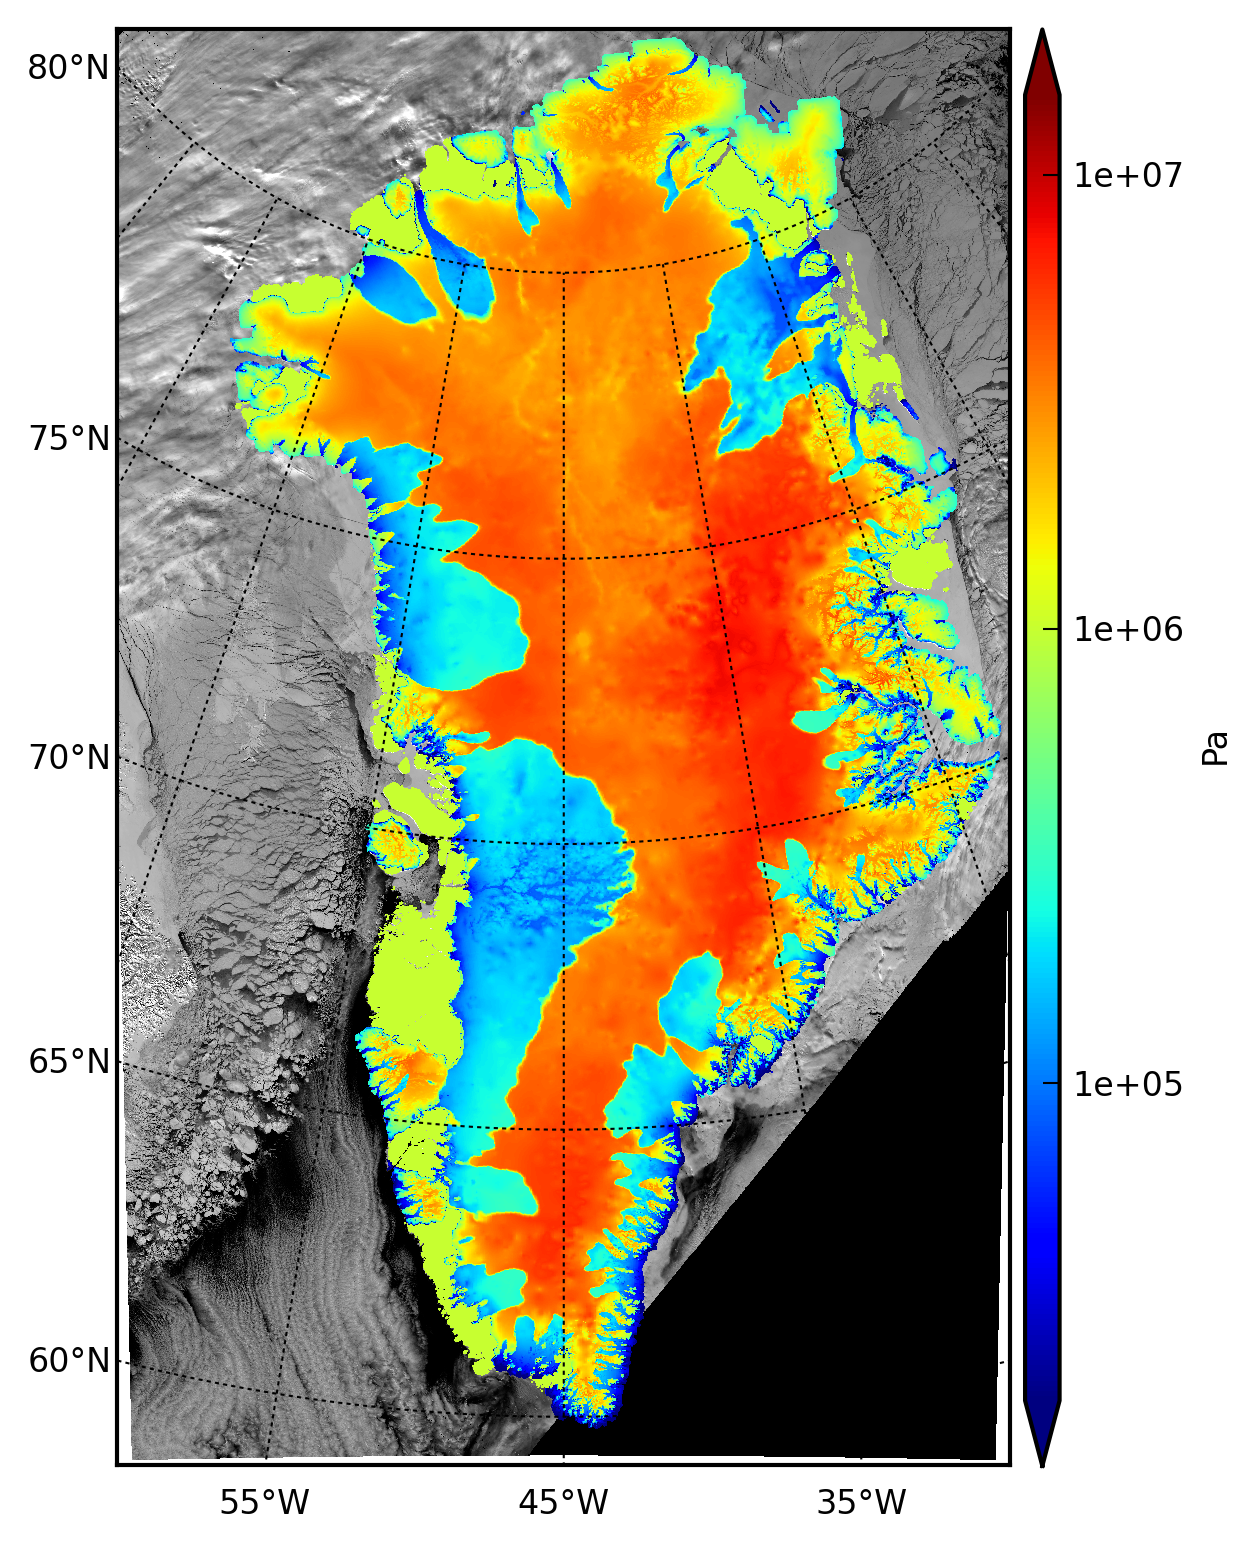
\includegraphics[width=\textwidth]{tauc}
      \end{figure}
    \end{column}
    \begin{column}{.54\linewidth}
      \begin{itemize}
      \item stresses vary by orders of magnitude
      \item basal hydrology, the glacier's ``plumbing system'' runs on a faster ime scale than ice flow
      \item despite more than 5 decades of research, we only have crude parametrizations
      \end{itemize}
    \end{column}
  \end{columns}
  \note[item]{First, stresses at the base vary by several orders of magnitude}
  \note[item]{depend on many factors, most importantly on the presence or absence of water}
  \note[item]{basal hydrology (the glacier's plumbing system) runs on a faster time scale than the ice flow itself}
  \note[item]{but the sub-glacial environment is not easy accessible}
  \note[item]{at the basal boundary, interactions between water flow, friction, heat flow, and sediment deformation is so complex that a deriving a theory from first principles is real challenge}
\end{frame}


\begin{frame}{Challenge: seaward margin boundary condition}
      \begin{figure}
        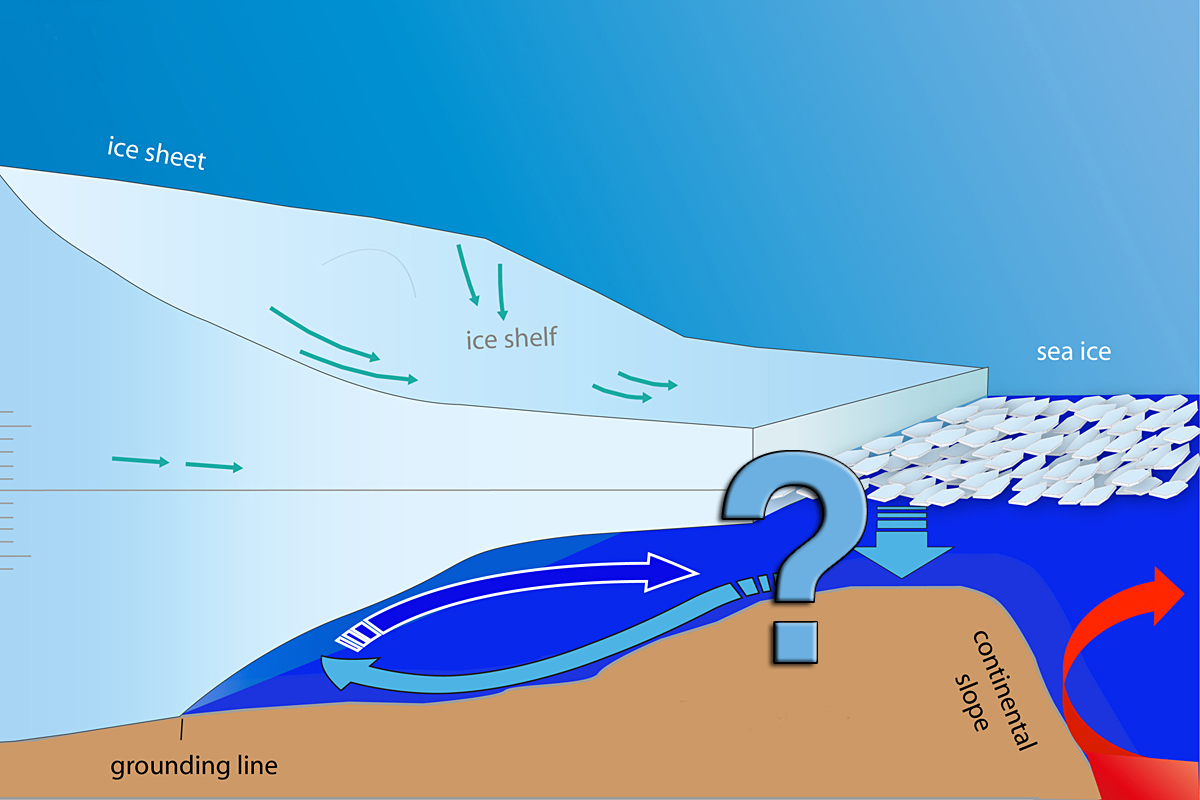
\includegraphics[width=.75\textwidth]{ice-shelf}
      \end{figure}
      \begin{itemize}
      \item ocean circulation $\Rightarrow$ basal melt rates
      \item calving mechanism
      \end{itemize}
      \note[item]{a big challenge is to understand how changing ocean currents and ocean temperatures affects sub-shelf basal melt rates}
      \note[item]{how this can weaken a shelf, and potentially lead to break up}
\end{frame}


\begin{frame}{Why ice sheet modeling is so hard}
    \begin{columns}[c]<1>
      \begin{column}{.28\linewidth}
        \begin{figure}
          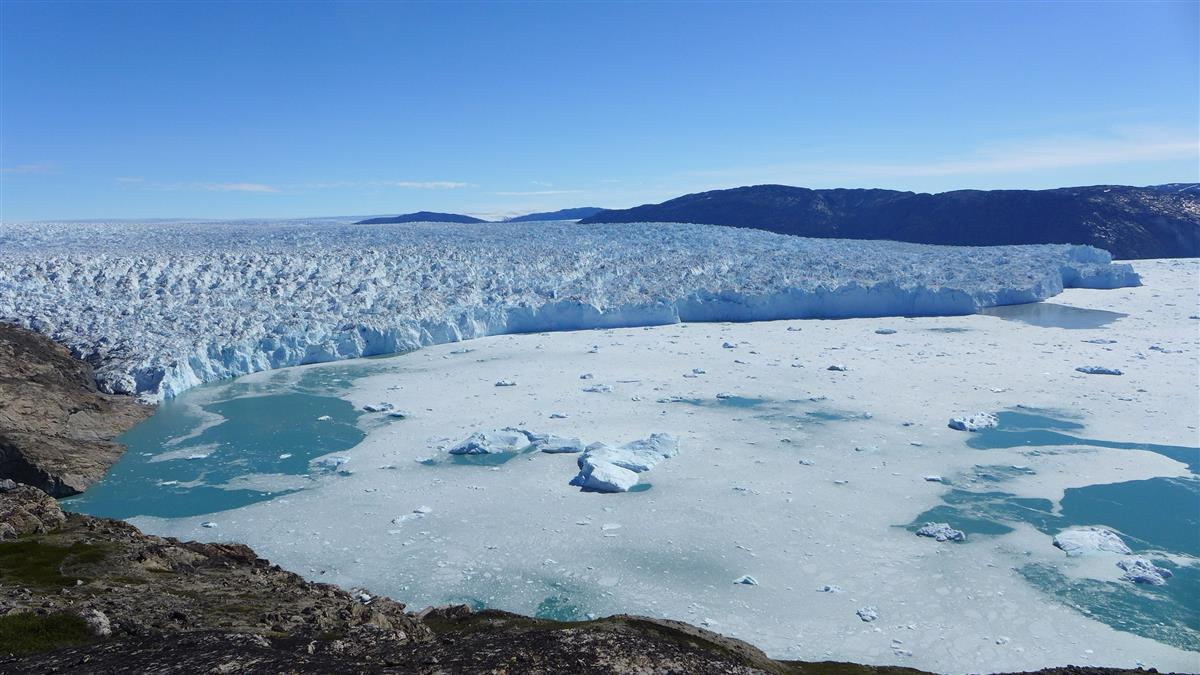
\includegraphics[width=\linewidth]{storeglacier}
        \end{figure}
      \end{column}
      \begin{column}{.67\linewidth}
        \begin{block}{Boundary conditions}
        \begin{itemize}
        \item seaward margin boundary condition
        \item basal boundary condition
        \end{itemize}
      \end{block}
      \end{column}
    \end{columns}
    \begin{columns}[c]<1-2>
      \begin{column}{.28\linewidth}
        \begin{figure}
          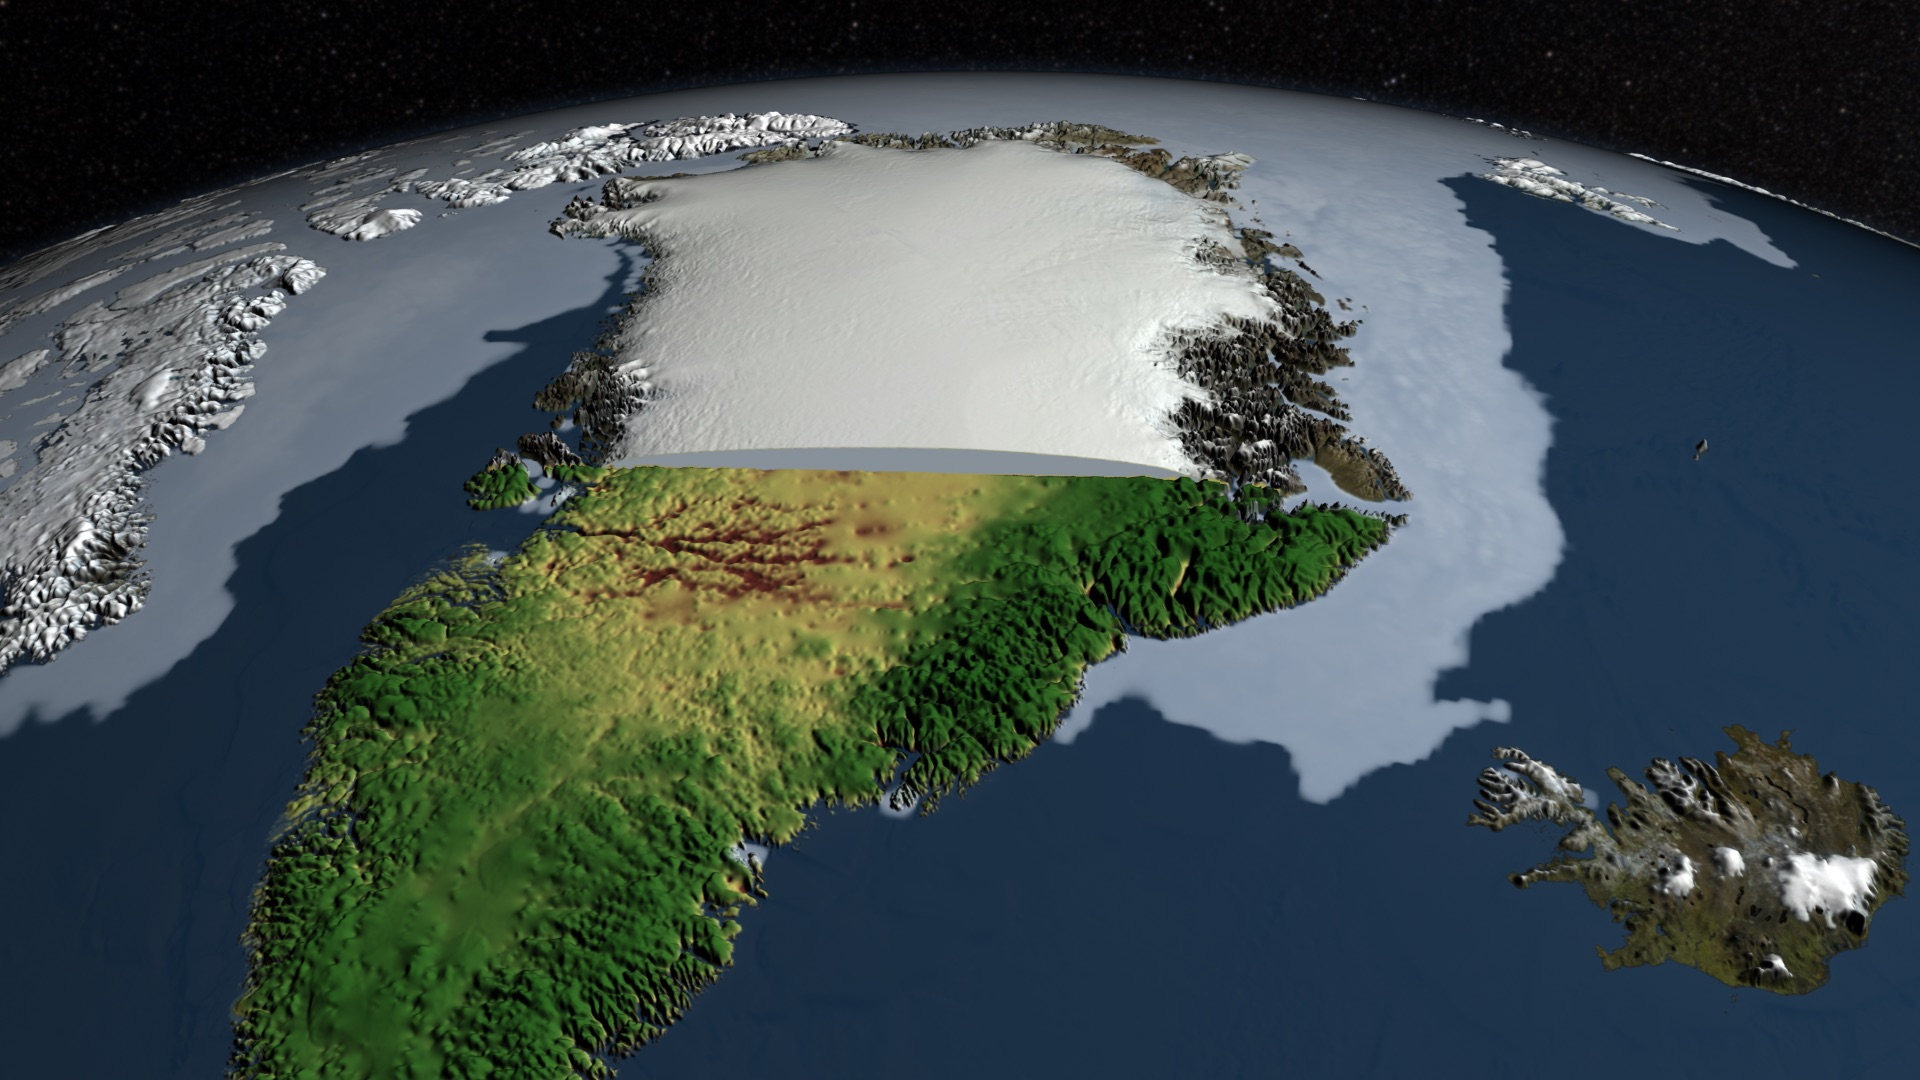
\includegraphics[width=\linewidth]{canale_grande_V05}
        \end{figure}
      \end{column}
      \begin{column}{.67\linewidth}
        \begin{block}{Initial conditions}
        \begin{itemize}
        \item ice thickness / subglacial topography is a first order constraint on ice flow
        \end{itemize}
      \end{block}
      \end{column}
    \end{columns}
    \begin{columns}[c]<1-3>
      \begin{column}{.3\linewidth}
        \begin{figure}
          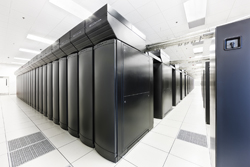
\includegraphics[width=\linewidth]{bw_front_sm}
        \end{figure}
      \end{column}
      \begin{column}{.67\linewidth}
        \begin{block}{Computational costs}
        \begin{itemize}
        \item solving the Stokes equations is computationally very expensive
        \end{itemize}
      \end{block}
      \end{column}
    \end{columns}
    \note<2->[item]{the main focus of my talk is on}
    \note<2->[item]{initial conditions and computational costs}
    \note<2->[item]{solving the Stokes equations is expensive}
\end{frame}


\begin{frame}{1. Simplify the Stokes equations}
  \begin{block}{Ice sheets are shallow}
    \begin{itemize}
    \item below in red is a no-vertical-exaggeration cross section of Greenland at $71^\circ$
      \small
    \item green and blue: standard vertically-exaggerated cross section
    \end{itemize}
    \begin{center}
      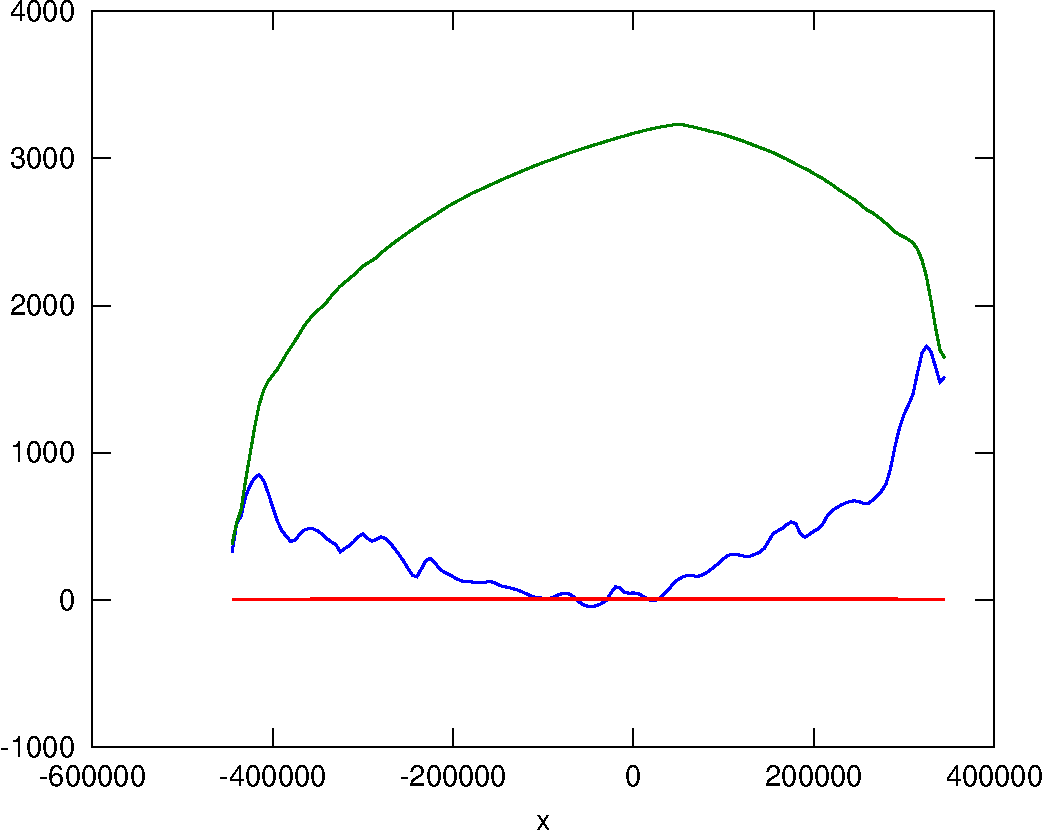
\includegraphics[width=0.4\textwidth]{green_transect} \\
      \footnotesize{Figure by E. Bueler}
    \end{center}
  \end{block}
\end{frame}

\begin{frame}{2. High Performance Computing (HPC)}
  \begin{block}{Exploit modern HPC through parallelism}
    \begin{figure}
      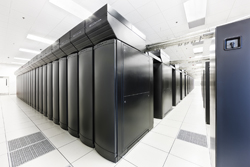
\includegraphics[width=5.5cm]{bw_front_sm}
      \hfill
      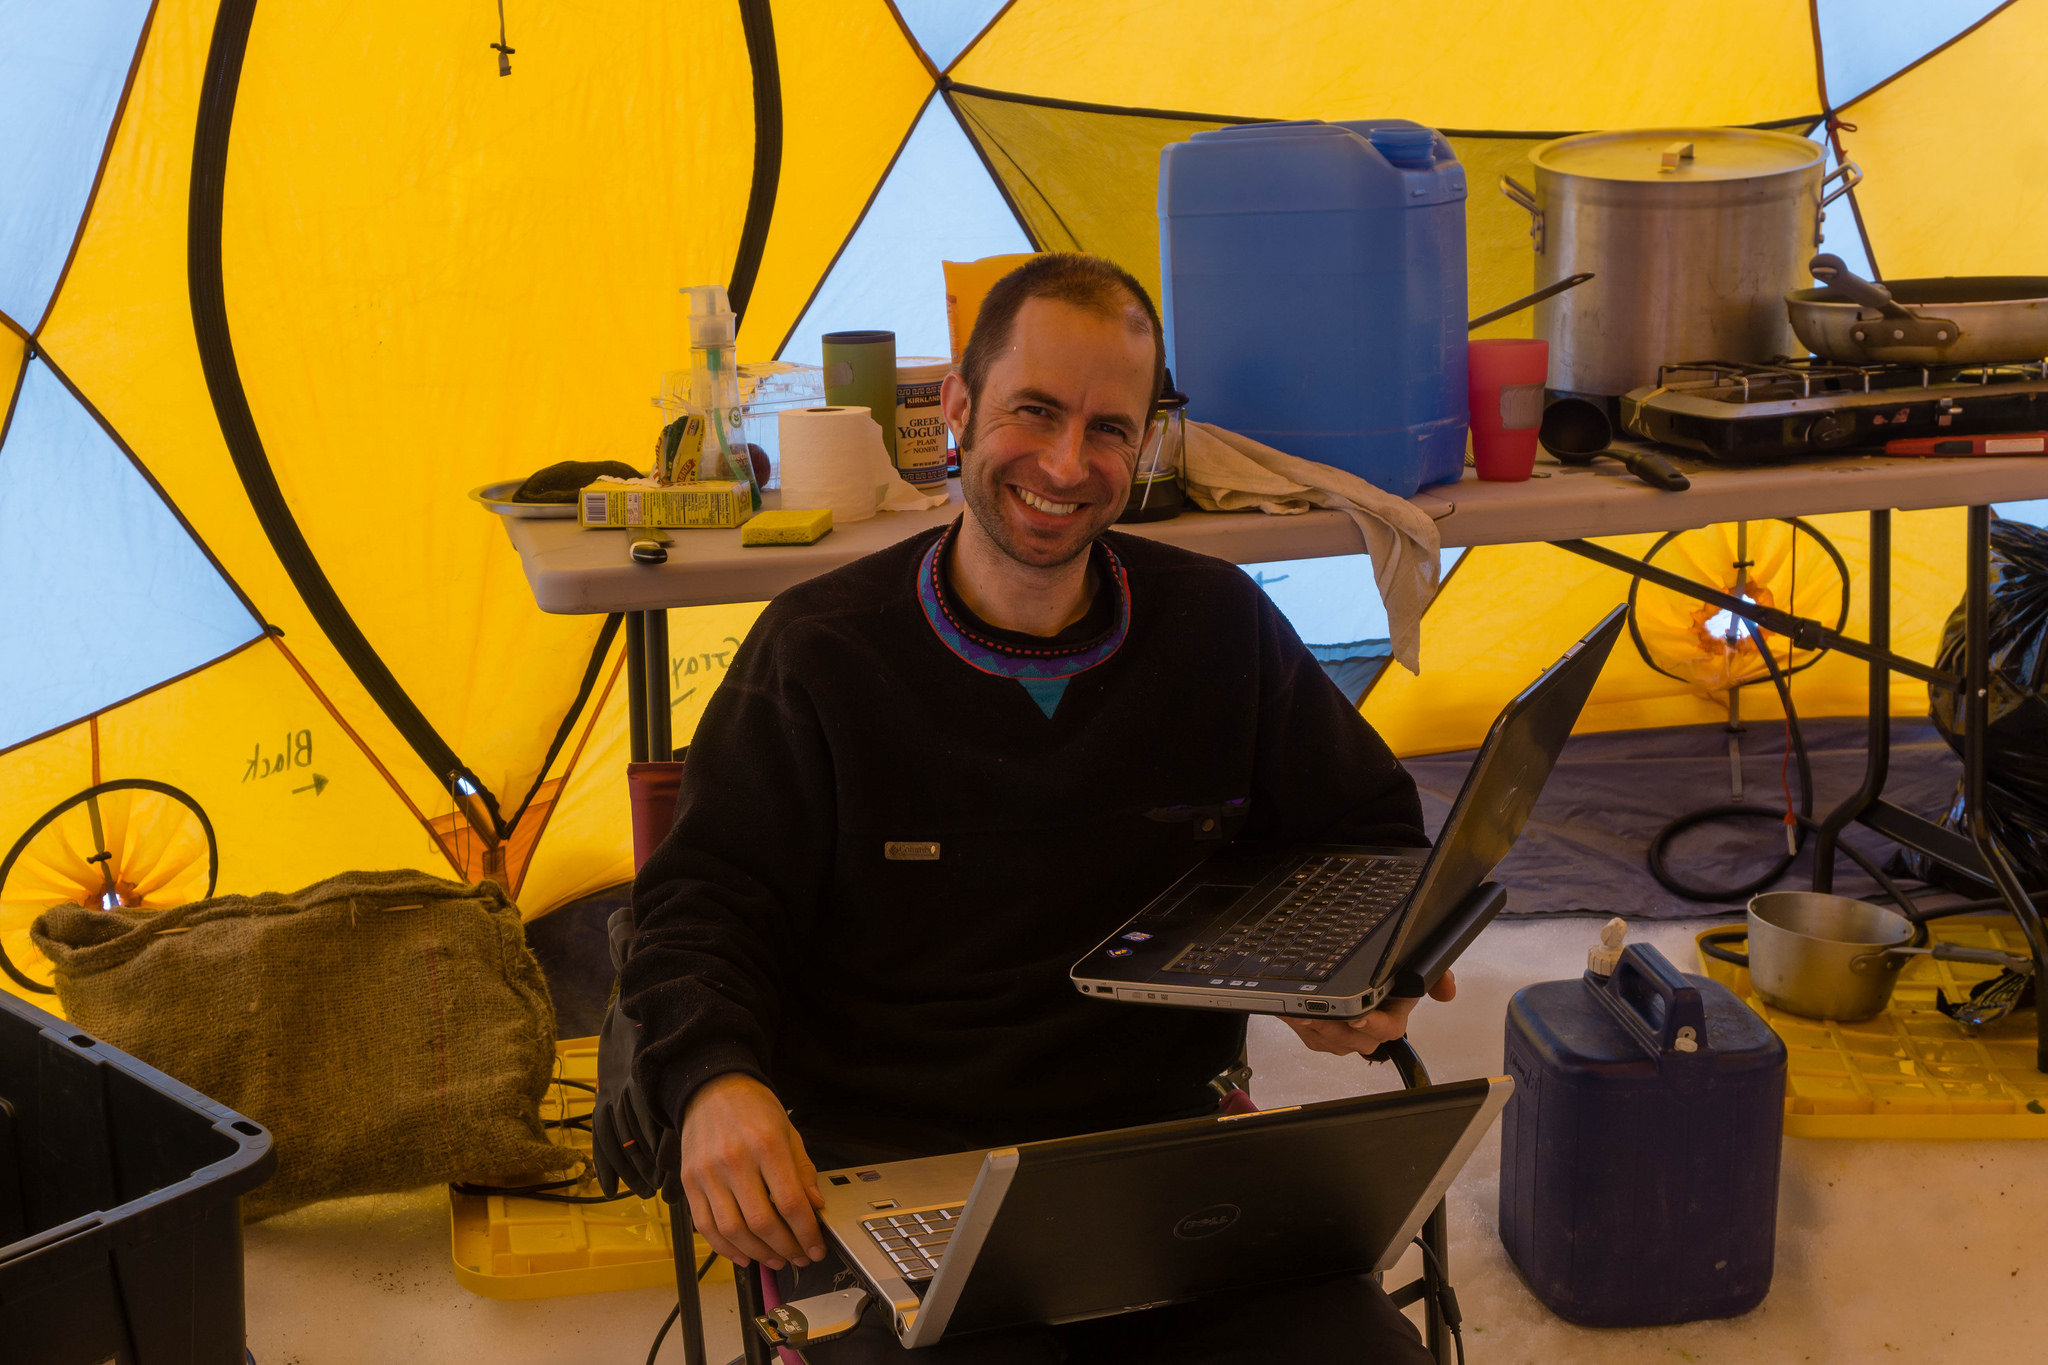
\includegraphics[width=5.5cm]{jason-parallel}
    \end{figure}
  \end{block}
\end{frame}


\begin{frame}{Parallel Ice Sheet Model (PISM)}
  
\includegraphics[width=4cm]{pism-logo}
  \begin{itemize}
  \item open-source, fully-parallel from start in 2006
  \item primary development at UAF, with global user base
  \item $>$100k lines of code; mostly C++
  \item NASA and NSF support
  \end{itemize}
  \begin{columns}
    \column[c]{4.75cm}
    \begin{figure}
      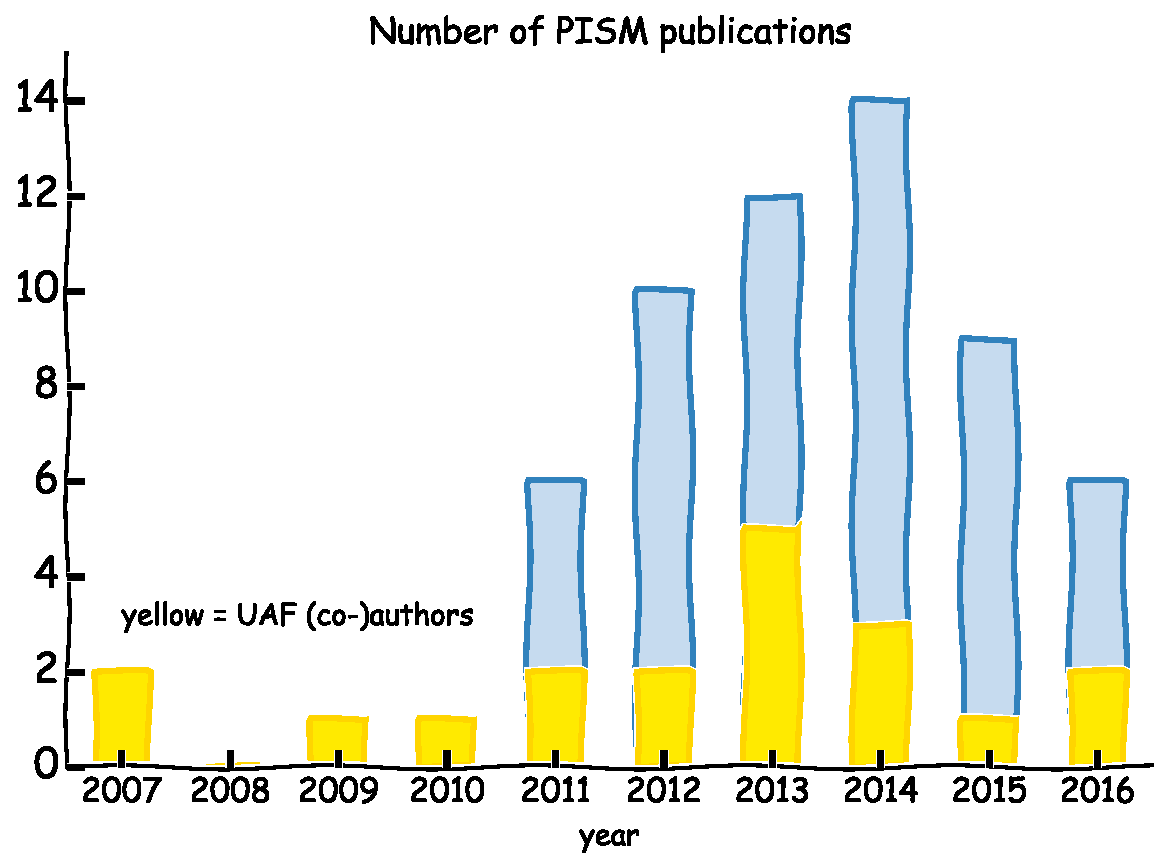
\includegraphics[width=\textwidth]{pism-uaf-publications}
    \end{figure}
    \column[c]{5cm}
    \includegraphics<1>[width=.7\textwidth]{pism-users}
  \end{columns}
\end{frame}

\begin{frame}{Parallel Ice Sheet Model (PISM) cont.}
  
\includegraphics[width=4cm]{pism-logo}
  \begin{itemize}
  \item PISM uses a computationally-efficient approximation to the Stokes equations
  \item PISM runs on large HPC systems
  \item simulations typically use 100-500 cores and may take up to two weeks wall time to complete
  \end{itemize}
\end{frame}


\begin{frame}{Why ice sheet modeling is so hard}
    \begin{columns}[c]<1>
      \begin{column}{.28\linewidth}
        \begin{figure}
          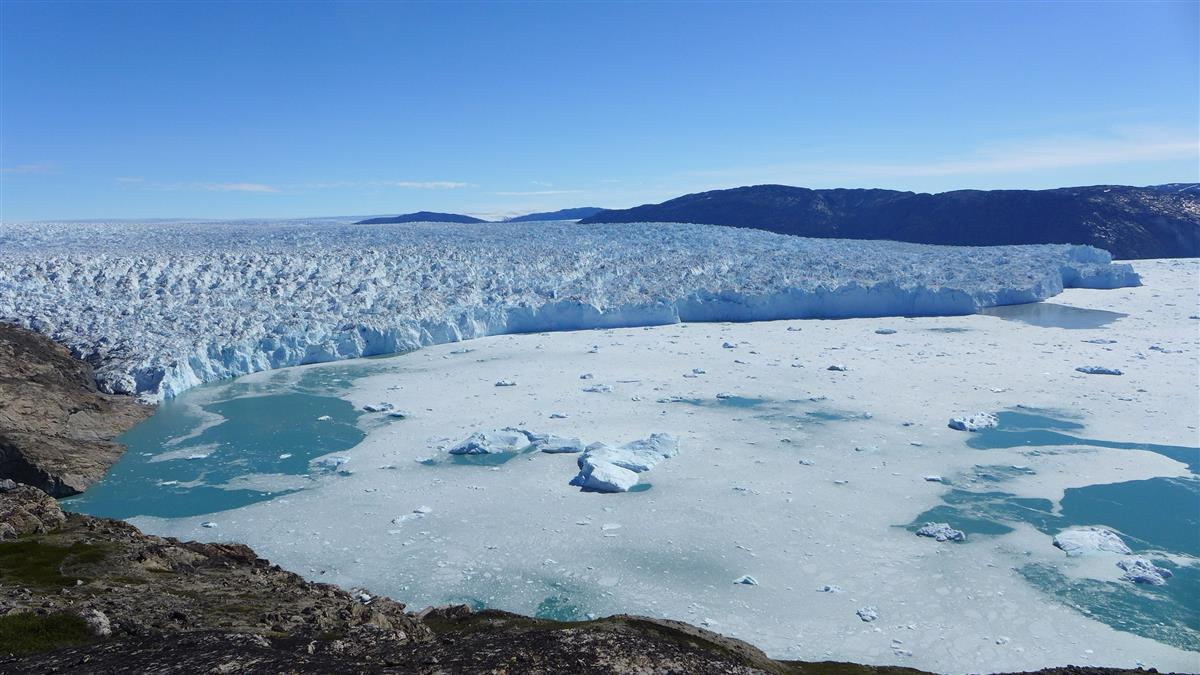
\includegraphics[width=\linewidth]{storeglacier}
        \end{figure}
      \end{column}
      \begin{column}{.67\linewidth}
        \begin{block}{Boundary conditions}
        \begin{itemize}
        \item seaward margin boundary condition
        \item basal boundary condition
        \end{itemize}
      \end{block}
      \end{column}
    \end{columns}
    \begin{columns}[c]<1-2>
      \begin{column}{.28\linewidth}
        \begin{figure}
          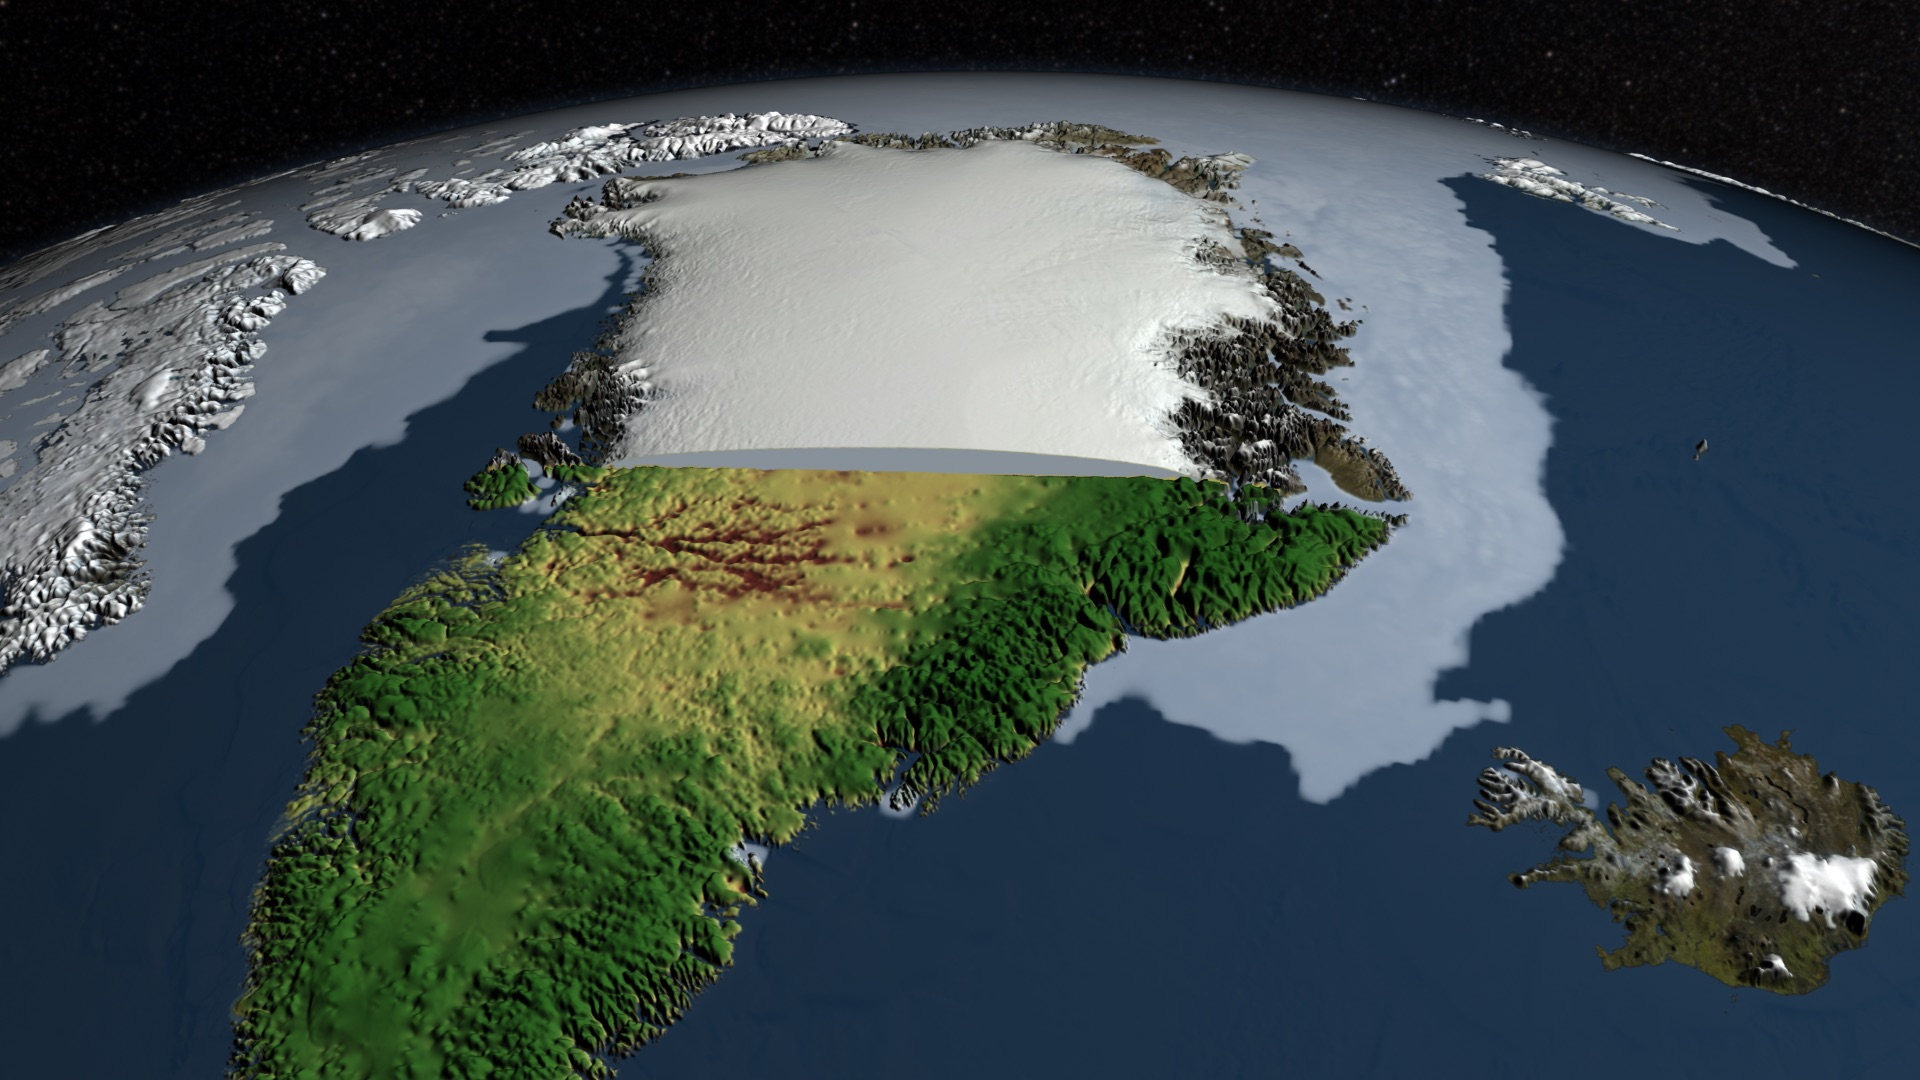
\includegraphics[width=\linewidth]{canale_grande_V05}
        \end{figure}
      \end{column}
      \begin{column}{.67\linewidth}
        \begin{block}{Initial conditions}
        \begin{itemize}
        \item ice thickness / subglacial topography is a first order constraint on ice flow
        \end{itemize}
      \end{block}
      \end{column}
    \end{columns}
    \begin{columns}[c]<1>
      \begin{column}{.3\linewidth}
        \begin{figure}
          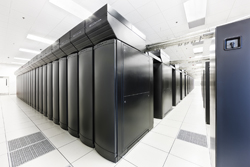
\includegraphics[width=\linewidth]{bw_front_sm}
        \end{figure}
      \end{column}
      \begin{column}{.67\linewidth}
        \begin{block}{Computational costs}
        \begin{itemize}
        \item solving the Stokes equations is computationally very expensive
        \end{itemize}
      \end{block}
      \end{column}
    \end{columns}
\end{frame}


\begin{frame}{Challenge: ice thickness}
  \begin{columns}
    \column[c]{1.25cm}
    
\includegraphics[width=\textwidth]{nasa-logo} \\
    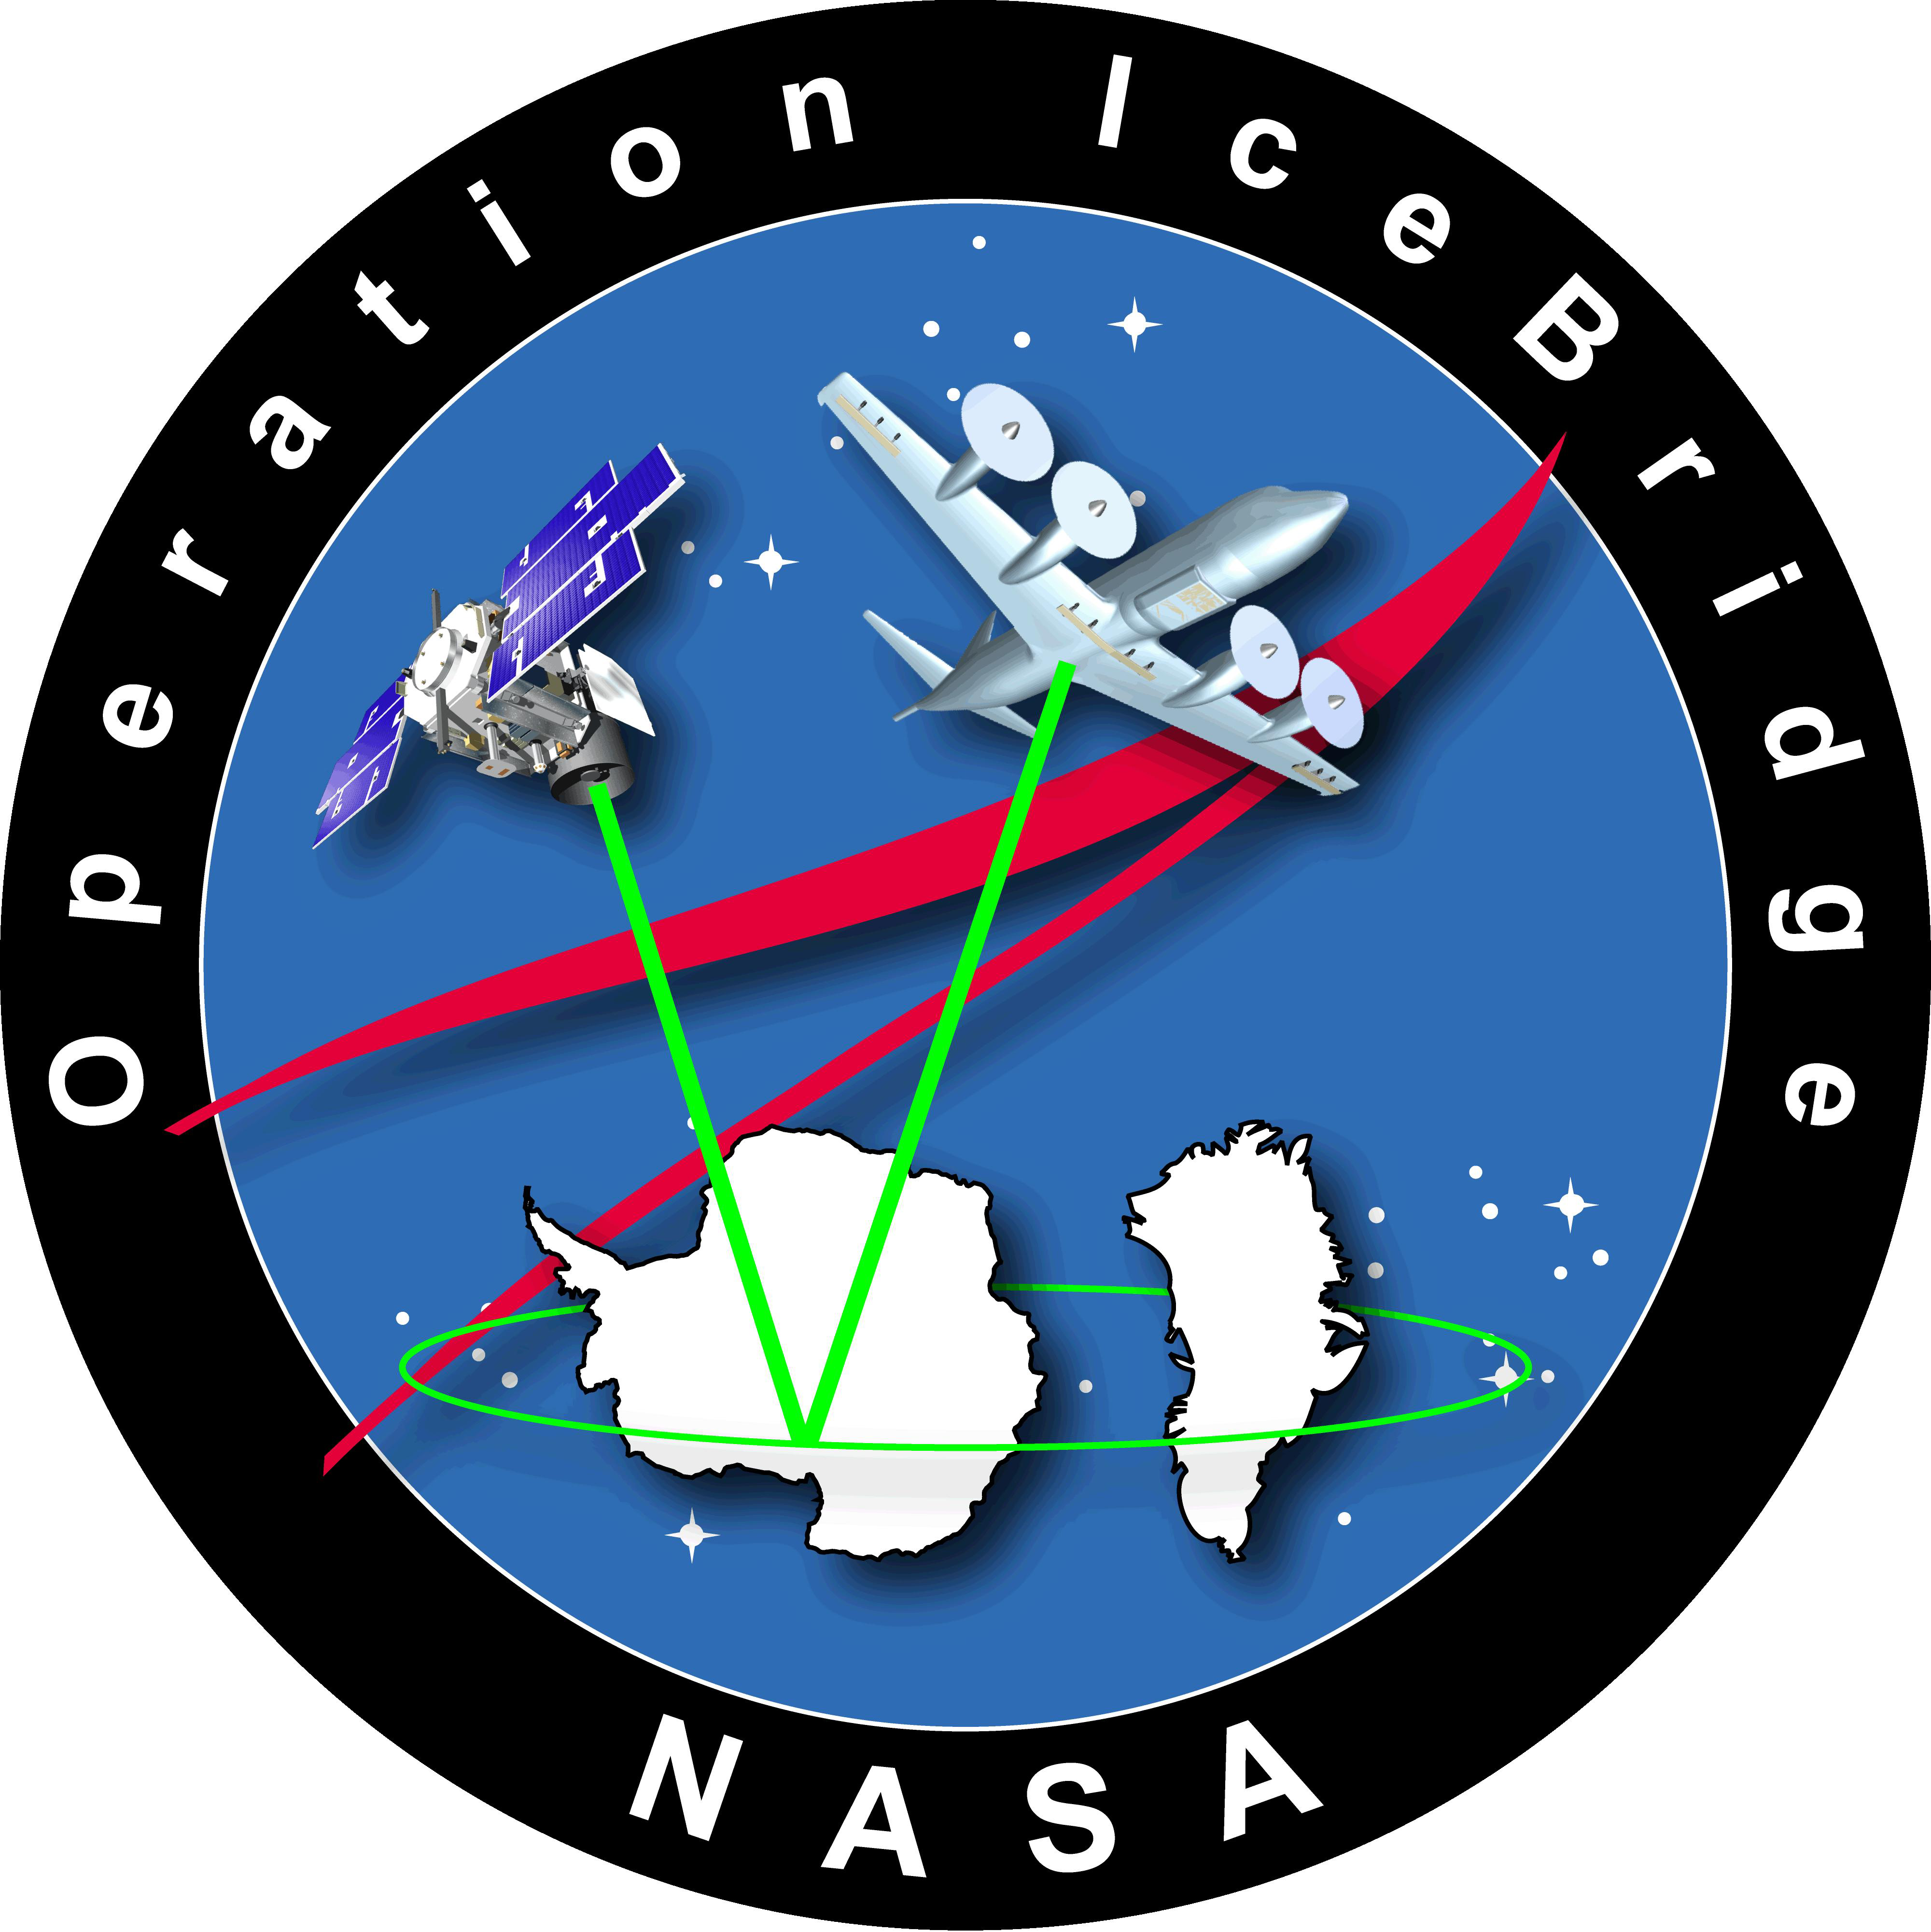
\includegraphics[width=\textwidth]{oib}
    \column[c]{10cm}
    \begin{itemize}
    \item ice thickness is a leading order constraint on ice flow
    \item but expensive to measure
    \item NASA realized that collecting a lot more ice thickness measurements is crucial to make ice sheet models better
    \item ice thickness measurements using the CReSIS radar became an important part of their Operation IceBridge mission (2009--today)
    \end{itemize}
  \end{columns}
  \begin{figure}
    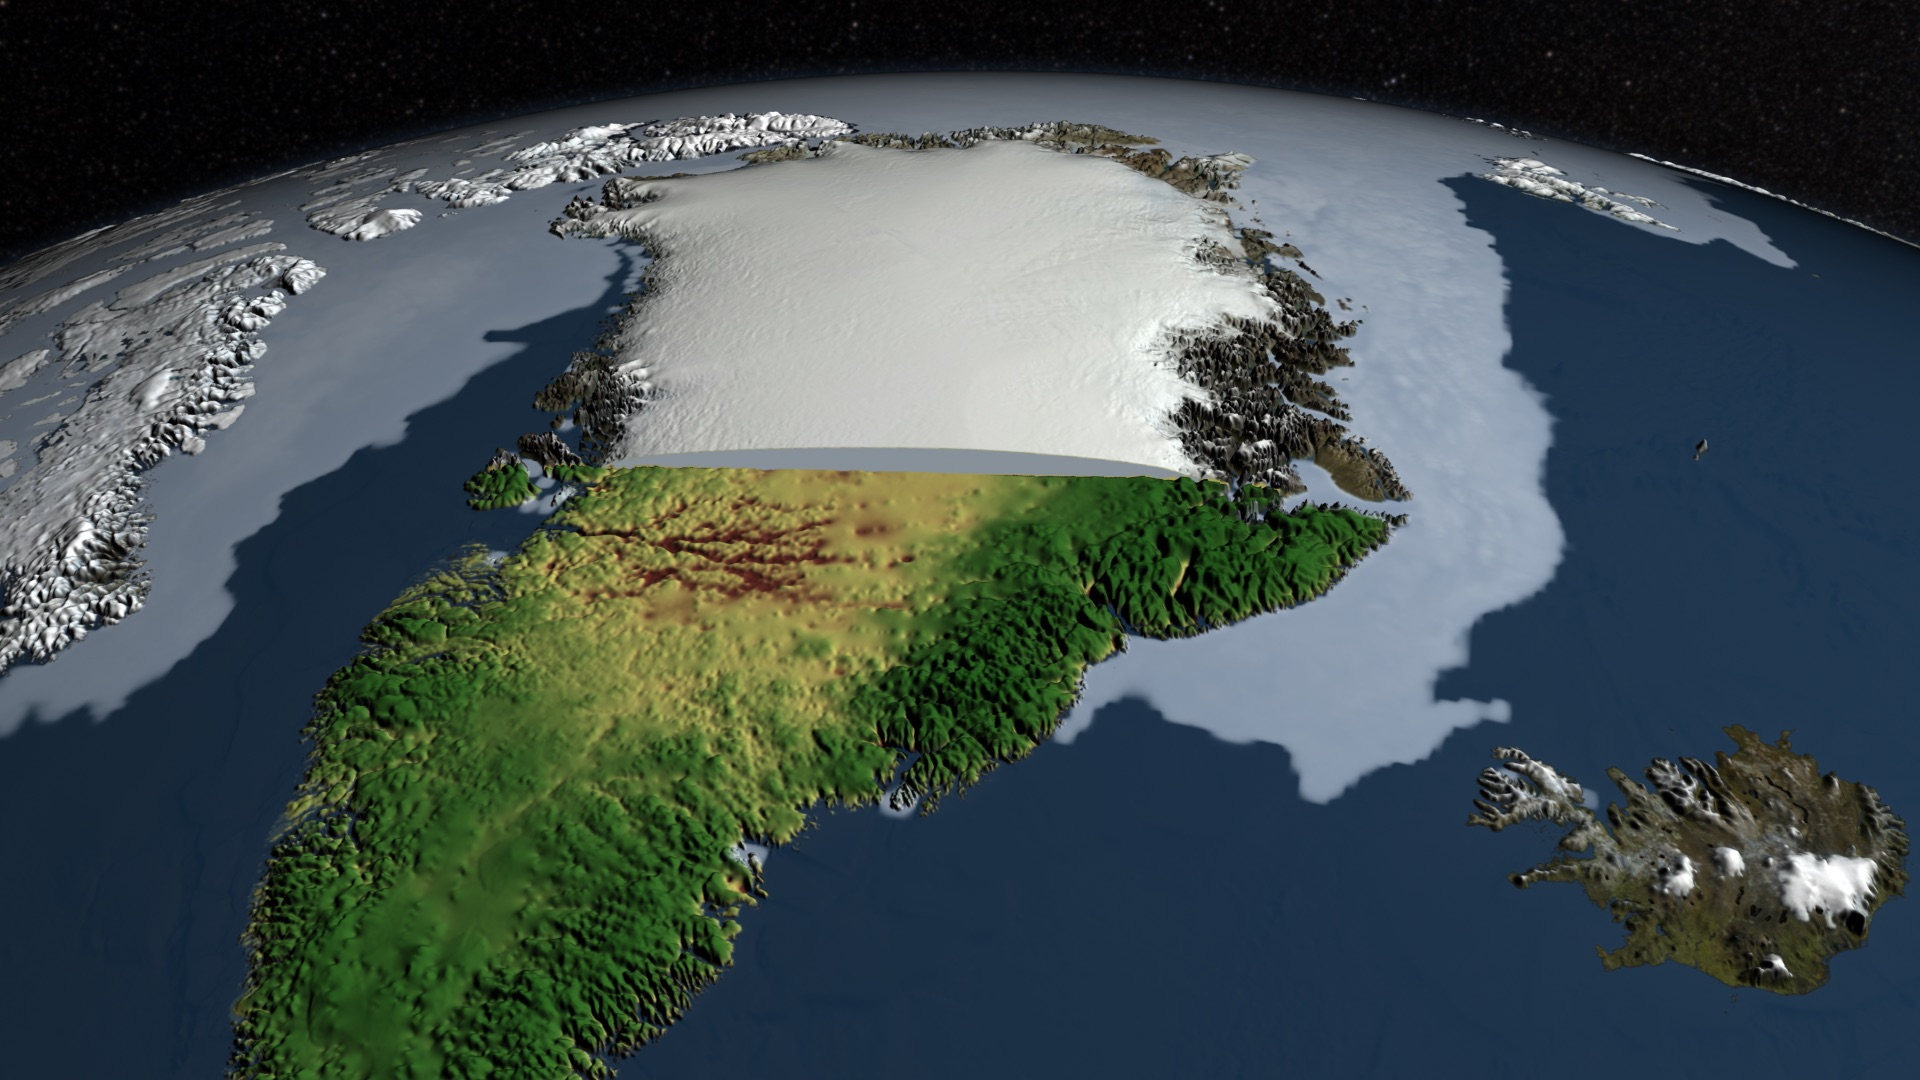
\includegraphics[width=6cm]{canale_grande_V05}
  \end{figure}
\note[item]{ice thickness is the difference between ice upper surface and the subglacial topography}
\end{frame}


\begin{frame}{NASA Operation IceBridge}
  \vspace{-0.74em}
  \begin{columns}
    \column[c]{4cm}
    \begin{itemize}
    \item additional flight lines since 2009
    \end{itemize}
    \column[c]{6cm}
    \begin{figure}
      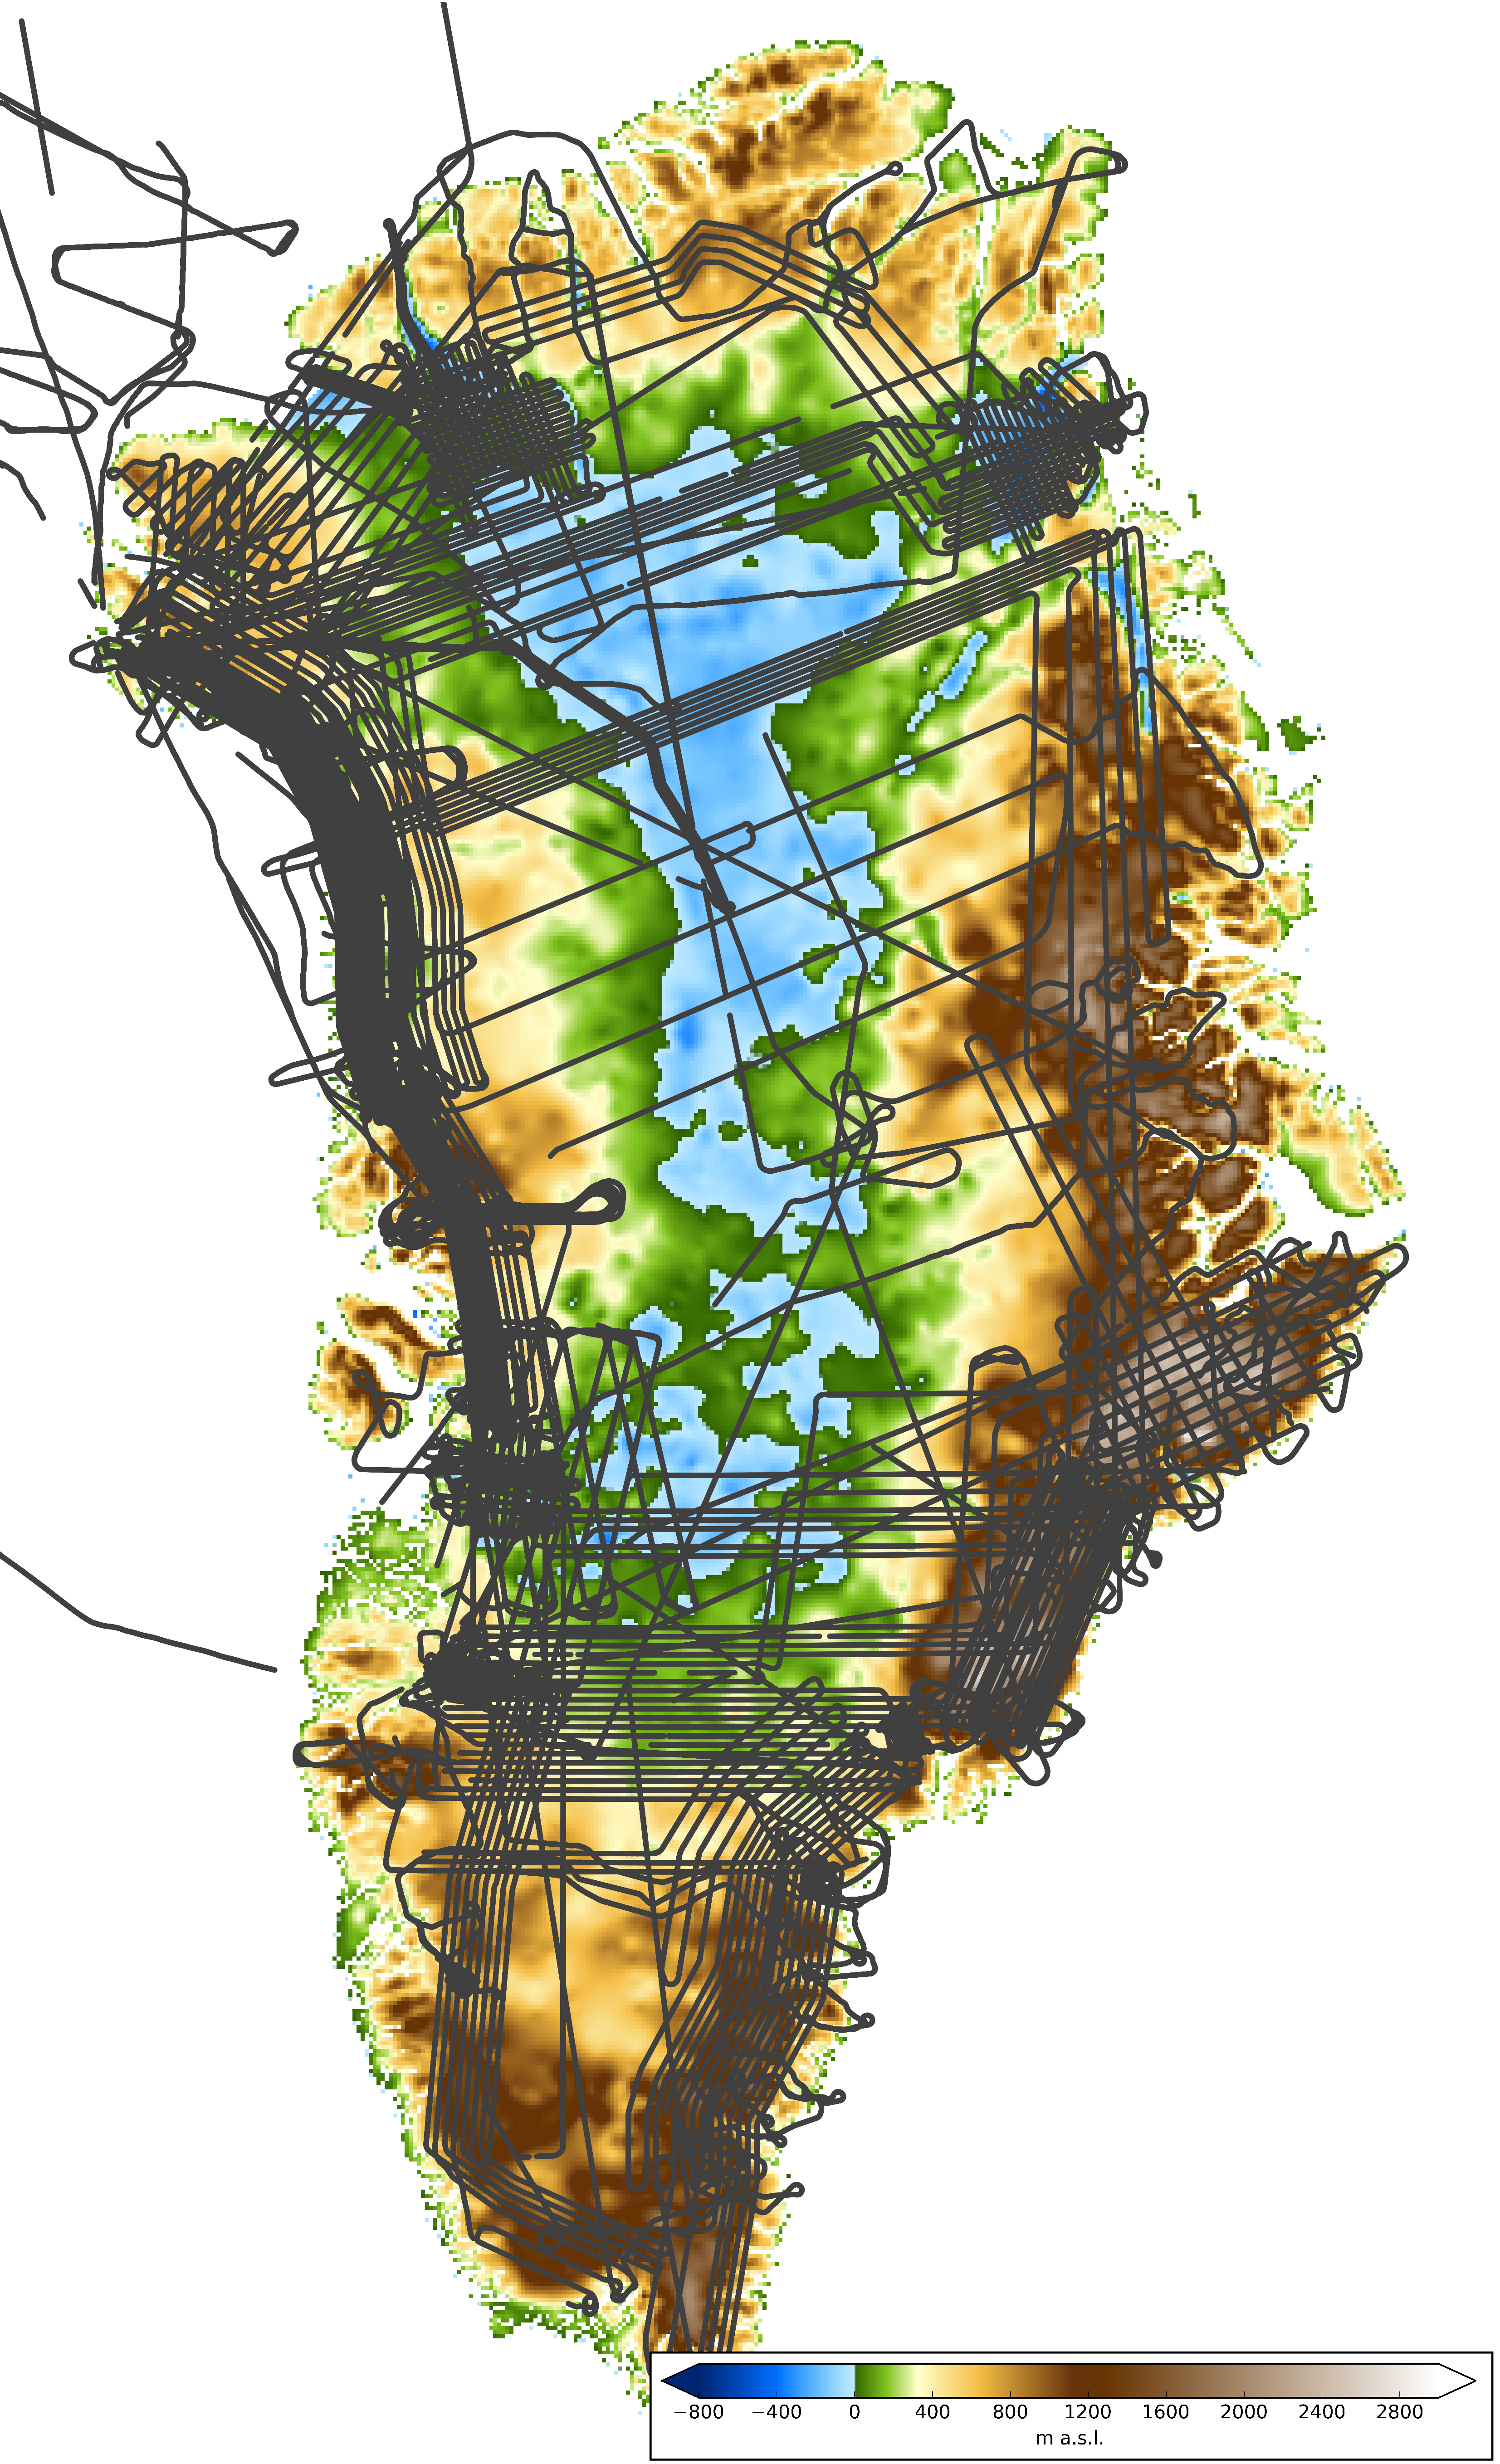
\includegraphics[height=8cm]{greenland-bed-old-oib}
    \end{figure}
  \end{columns}
\end{frame}

\begin{frame}{Zoom in to Jakobshavn Isbr{\ae}}
  \begin{figure}
    \small{old (2001) \hspace{5em} new (2014)}
    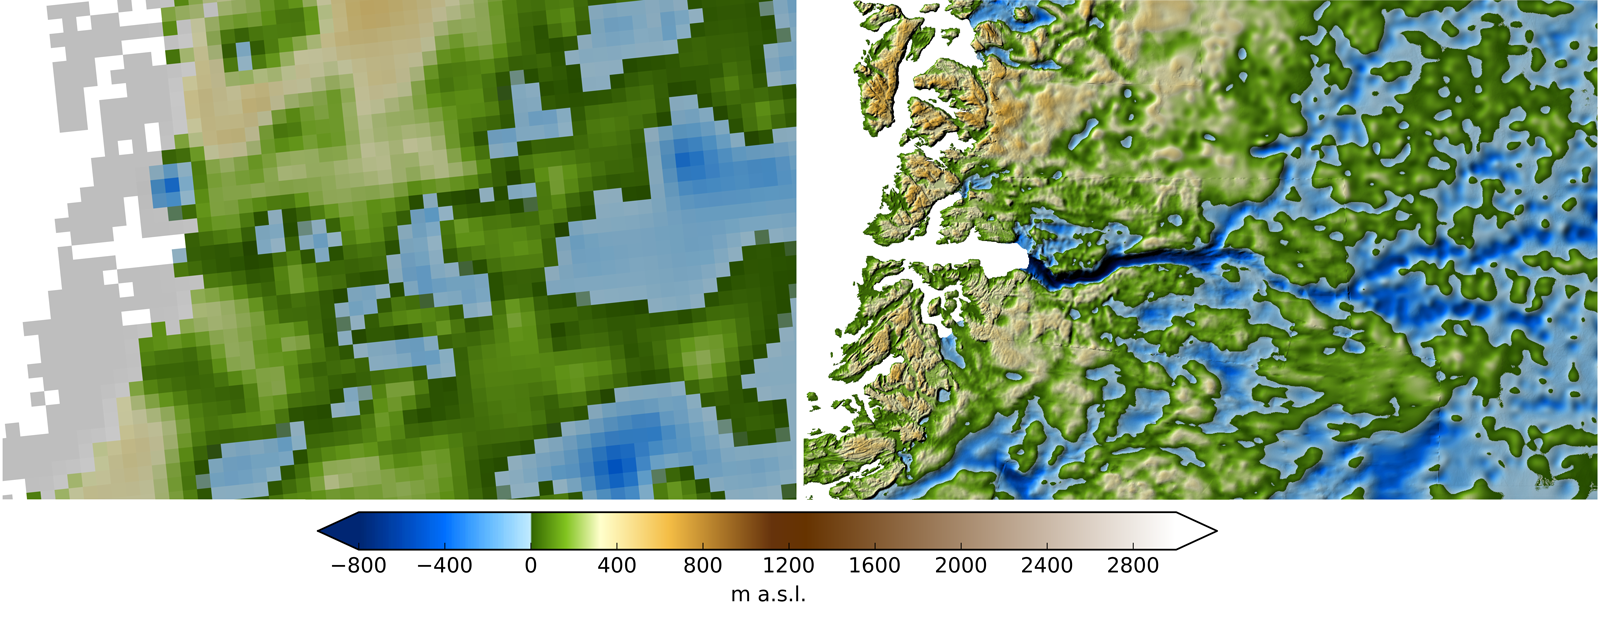
\includegraphics[width=12cm]{jako_bed}
 \end{figure}
\end{frame}


\begin{frame}{NASA Operation IceBridge}
  \begin{columns}
    \column[c]{8cm}
    \begin{figure}
      \small{old (2001) \hspace{4em} new (2014)}
      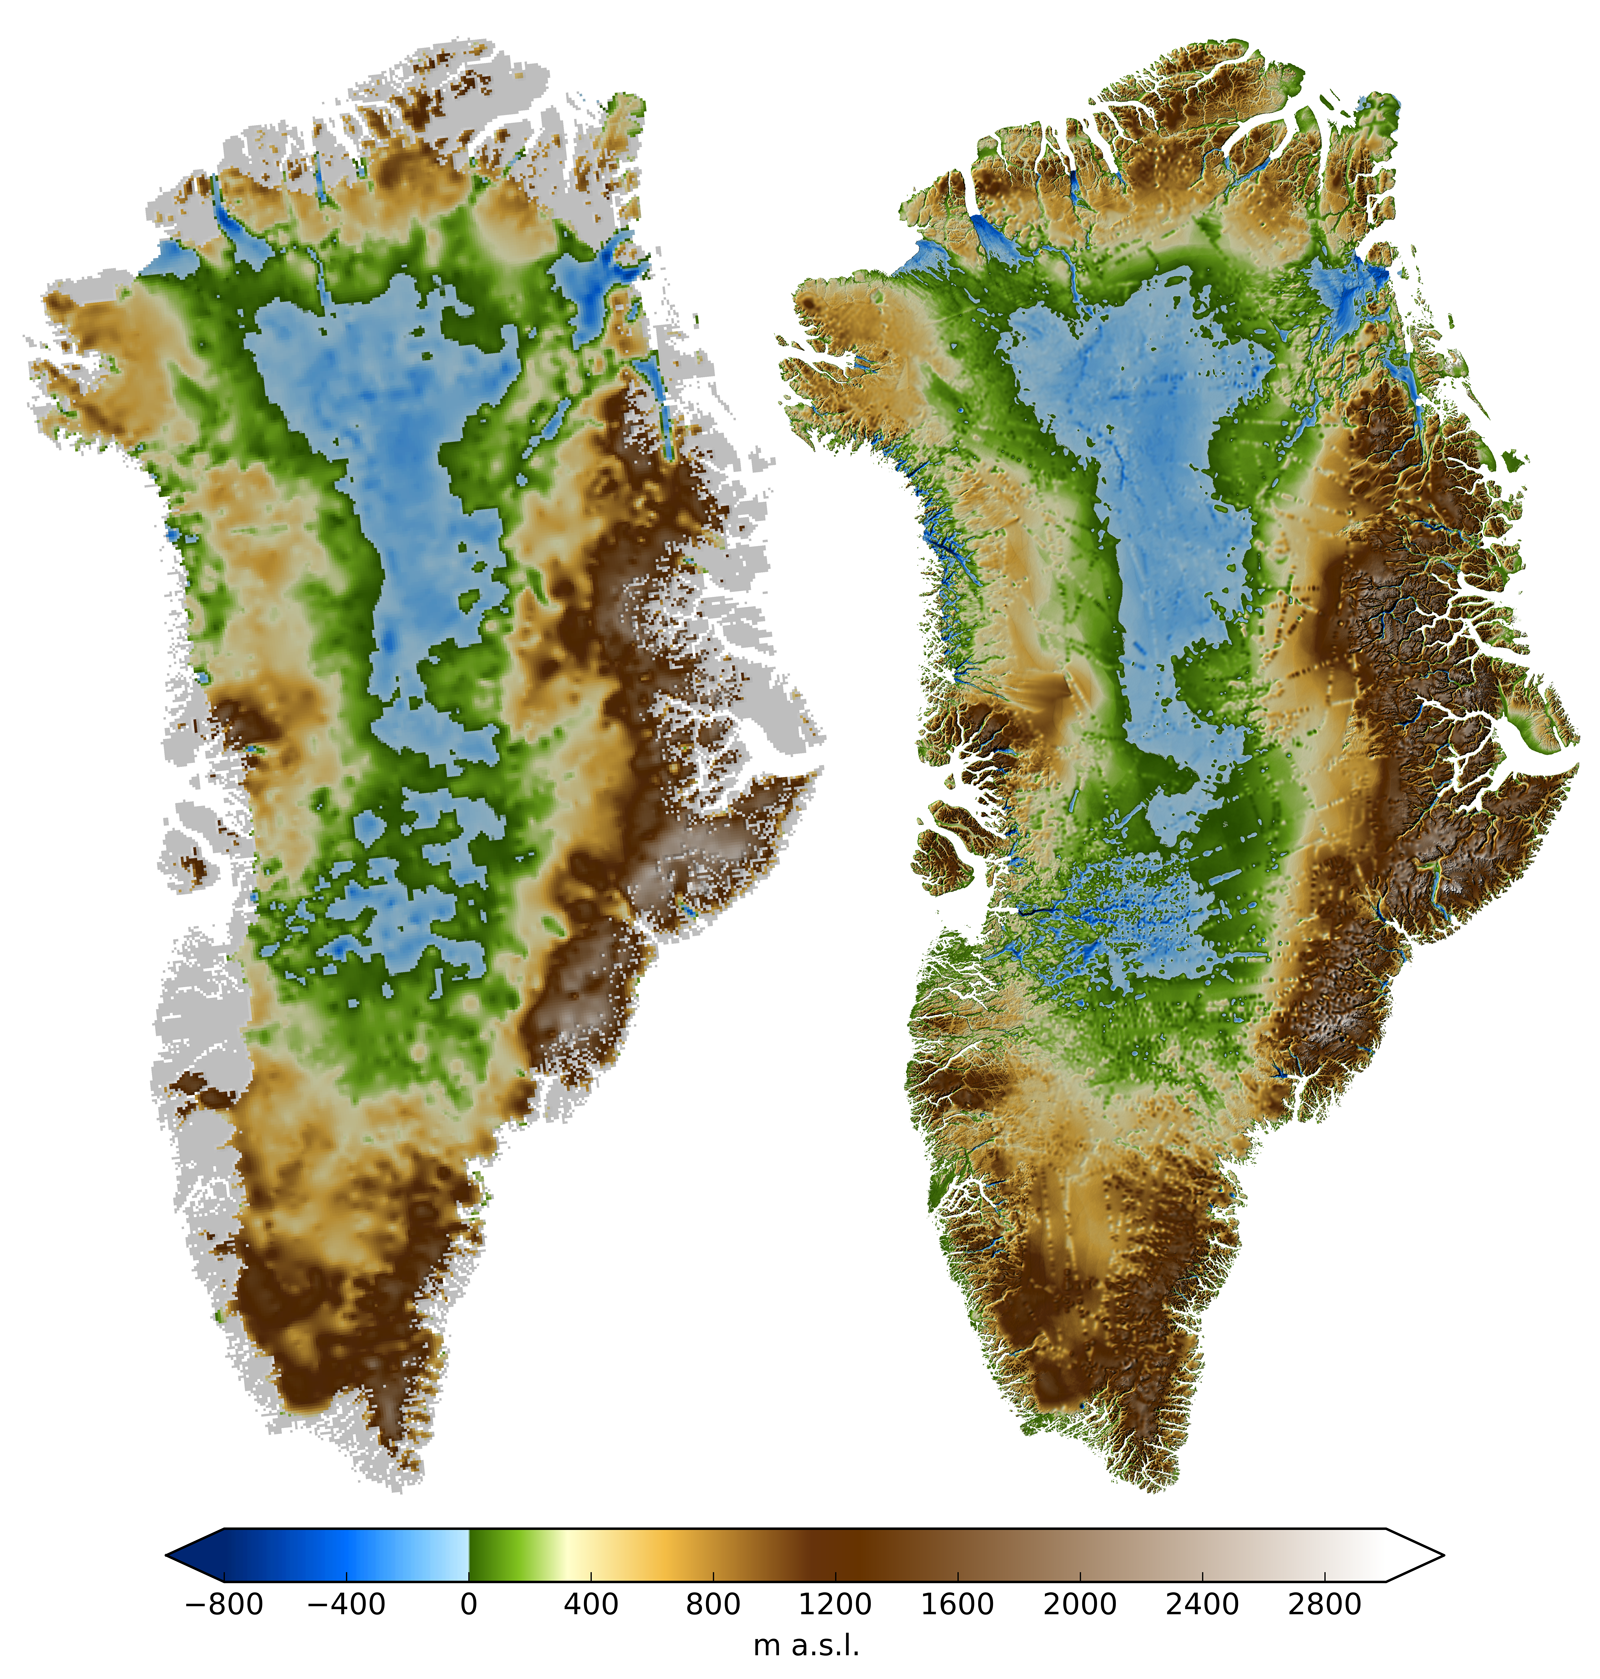
\includegraphics[height=7.5cm]{greenland_bed}
    \end{figure}
    \column[c]{4cm}
    \begin{itemize}
    \item from 5\,km to 150\,m horizontal grid resolution
    \end{itemize}
  \end{columns}
\end{frame}

\begin{frame}{NASA Operation IceBridge}
  \begin{figure}
    \includegraphics[height=2.5cm]{nasa-logo} \qquad
    \includegraphics[height=2.5cm]{oib} \qquad
    \includegraphics[height=2.5cm]{1000-dollar-bills}
  \end{figure}
  \begin{itemize}
  \item do NASA's OIB million\$ really make ice sheet models better?
  \end{itemize}
  \note[item]{so the multi million dollar question is}
  \note[item]{does this investment pay off?}
\end{frame}


\begin{frame}{Observed flow speeds}
\vspace{-0.74em}
  \begin{columns}
    \column[c]{5cm}
    \begin{figure}
      \includegraphics[width=\textwidth]{greenland-obs-overview}
    \end{figure}
    \column[c]{5cm}
    \only<1>{Jakobshavn Isbr{\ae}}
    \includegraphics<1>[width=\textwidth]{jakobshavn-obs-nogate}
    \only<1>{\\ {} }
  \end{columns}
  \note[item]{let's look at JIB again}
  \note[item]{observations show strongly channelized flow}
  \note[item]{with high flow speeds in the center}
\end{frame}


\begin{frame}{Ice thickness and simulated flow speeds}
\vspace{-0.74em}
  \begin{columns}
    \column[c]{5cm}
    \begin{figure}
      \includegraphics<1-2>[width=\textwidth]{greenland-obs-basal-overview}
      \includegraphics<3-4>[width=\textwidth]{greenland-obs-basal-overview-mo14}
    \end{figure}
    \column[c]{5cm}
    \only<1,3>{Jakobshavn Isbr{\ae}}
    \only<2>{no fast flow}
    \only<4>{fast flow appears}
    \includegraphics<1>[width=\textwidth]{jakobshavn-bed-5000m-ba01}
    \includegraphics<2>[width=\textwidth]{jakobshavn-speed-exp-4500m-ba01}
    \includegraphics<3>[width=\textwidth]{jakobshavn-bed-mo14}
    \includegraphics<4>[width=\textwidth]{jakobshavn-speed-exp-600-v1.2-no-scale-no-gate}
    \only<1>{\\ 5\,km, old data set (2001)}
    \only<2,4>{\\ simulated surface speed}
    \only<3>{\\ 600\,m, new data set (2014)}
  \end{columns}
  \note<1>[item]{now let's do a simualulation with the old ice thickness data}
  \note<2>[item]{there isn't really any fast flow}
  \note<3>[item]{now use the new ice thickness}
  \note<4>[item]{and we get fast flow}
\end{frame}


\begin{frame}{Can we capture the present-day flow field?}
  \begin{figure}
    \includegraphics[height=7cm]{greenland-overview-3}
    \\ \scriptsize{Aschwanden, Fahnestock, Truffer (2016) \textit{Nature Communications}}
  \end{figure}
  \note[item]{first time capturing the flow field for the right reason}
  \note[item]{this is quite a break through in ice sheet modeling}
  \note[item]{though not a surprising one}
  \note[item]{it just confirms what students learn in glaciology 100:}
  \note[item]{ice flows downhill}
\end{frame}


\begin{frame}
  \frametitle{Estimating future sea-level rise}
  \begin{figure}
    \includegraphics[height=6cm]{grn1km_speed_slr}
  \end{figure}
\end{frame}



\begin{frame}
  \frametitle{The next thousand years}
  \begin{figure}
   \movie[showcontrols=true,autostart,loop,width=12cm]{\includegraphics[width=12cm]{../movies/gris-g1200m_rcps-hd1920}}{../movies/gris-g1200m_rcps-hd1920.mov}
  \end{figure}
\end{frame}


\begin{frame}
  \frametitle{In a thousand years}
  \begin{figure}
    \includegraphics[height=8cm]{rcp-final-states-composite}
  \end{figure}
\end{frame}

\begin{frame}
  \frametitle{The next thousand years}
  \begin{figure}
    \includegraphics[height=8cm]{les-composite}
  \end{figure}
\end{frame}


\end{document}